\chapter{RESULTS} \label{results}

The principle results reported by this analysis are the discovery significance and an estimate of the signal strength $\mu$ of the \VHbb\ decay. The discovery significance is the statistical significance of any observed excess of events in data over the expected SM background. The signal strength is defined as the measured production cross section times the \Htobb\ branching fraction divided by the expected SM value or $\sigma / \sigma_{\textrm{SM}}$. The statistical analysis was performed using the \textsc{combine}\cite{HIGGSCOMBINE} software package developed by the CMS collaboration which provides a command line interface for the statistical tools implemented in \textsc{RooFit}\cite{ROOFIT} and \textsc{RooStats}\cite{ROOSTATS}.

\section{Statistical Treatment}

The discovery significance is computed using the profile likelihood asymptotic approximation.\cite{STATS1,FITRES2,FITRES3,FITRES4} In this approach, the significance is calculated from a profile likelihood ratio where the signal strength is set to zero in the numerator and is allowed to float freely in the denominator. The test statistic defined by the profile likelihood ratio is thus
\begin{equation}
  q_{0} = -2 \ln \frac{\mathcal{L}\left( \textrm{data} | b, \hat{\theta}_{0} \right)}{\mathcal{L}\left( \textrm{data} | \hat{\mu} \times s + b, \hat{\theta} \right)}\ \mathrm{for}\ \hat{\mu} > 0,
  \label{eq:proflikeapprox}
\end{equation}
where $\textrm{data}$ comes from either the observed dataset when calculating the observed significance or a generated toy dataset when calculating the expected significance, $s$ and $b$ are respectively the expected number and distribution of signal and background events, $\hat{\theta}_{0}$ is the estimated value of the nuisance parameter that maximizes the likelihood of the numerator, and $\hat{\mu}$ and $\hat{\theta}$ are the estimated values of the signal strength and nuisance parameter that maximizes the likelihood of the denominator. The value of $\hat{\mu}$ is restricted to be positive to remain physically meaningful. Assuming that the number of events is large, the distribution of this test statistic may be determined asymptotically using Wilke's theorem.

The local $p$-value is defined as the probability of obtaining a value of $q_{0}$ greater than or equal to the value of $q_{0}$ observed in data under the background-only hypothesis such that
\begin{equation}
  p_{0} = P\left( q_{0} \geq q_{0}^{\textrm{data}} | b \right).
  \label{eq:localpvalue}
\end{equation}
The value of $p_{0}$ is therefore a measure of the probability that an upward fluctuation of the background is responsible for an observed excess of events in the absence of signal. Each value of $p_{0}$ corresponds to a unique level of significance $z$ that is computed from the right-sided tail of a standard normal distribution
\begin{equation}
  p_{0} = \frac{1}{\sqrt{2\pi}} \int_{z}^{+\infty} e^{-\frac{1}{2} x^{2}} dx.
  \label{eq:zscore}
\end{equation}
This discovery significance is typically quoted in terms of the number of standard deviations $\sigma$, with a threshold of $3\sigma$ ($z = 3$) required to establish evidence for a decay and a threshold of $5\sigma$ ($z = 5$) required to establish an observation of a decay.

In the presence of an excess of events, the best fit value of the estimated signal strength $\hat{\mu}$ is determined by a simultaneous binned maximum likelihood fit over the signal and control regions of all decay channels during which the signal strength $\hat{\mu}$ is allowed to vary freely and the nuisance parameters $\hat{\theta}$ vary within their uncertainties. For the \VHbb\ analysis, the signal extraction fit is performed using the DNN-based multivariate discriminants in the signal regions and the distributions of the subleading DeepCSV score of the two \qrkb-jets \btagmin\ in the control regions. The signal extraction fit for the \VZbb\ cross-check analysis proceeds in the same manner, with the only differences being a wider dijet invariant mass window in the signal region and a DNN classifier trained to identify diboson events as signal. For the dijet invariant mass cross-check analysis, the fit is performed using the dijet invariant mass distributions of the four distinct categories in the signal region of each decay channel while the control regions and their distributions remain the same as in the \VHbb\ analysis.

\section{\VZbb\ Analysis}

The data to MC scale factors obtained by the maximum likelihood fit are shown in Table \ref{tbl:SFVZbb}. The post-fit multivariate discriminant distributions of each channel are shown individually in Figure \ref{fig:SRVZbb} and combined in Figure \ref{fig:SBVZbb}. The expected post-fit significance of the excess over the background prediction is $5.0\sigma$, while the observed significance is $5.2\sigma$. The best fit signal strength is $\mu = 1.05_{-0.21}^{+0.22}$ for all channels combined and the signal strengths of the individual channels, shown in Figure \ref{fig:MuVZbb}, are compatible with a $p$-value of 64\%. These results are in good agreement with past measurements of the \VZbb\ process and the observation of this known Standard Model process serves as an important validation of the analysis strategy.

\begin{table}[htbp]
  \caption[\VZbb\ Analysis Scale Factors]{The data to Monte-Carlo scale factors obtained by the simultaneous maximum likelihood fit over all \VZbb\ channels. The errors include both statistical and systematic uncertainties.}
  \label{tbl:SFVZbb}
  \begin{tabularx}{6.5in}{lXXll}
    \hline
    Process       & \ZnnH           & \WlnH           & \ZllH, Low \pT(\bosV) & \ZllH, High \pT(\bosV) \\
    \hline
    \Wlight       & $1.04 \pm 0.01$ & $1.04 \pm 0.01$ & -                     & -                      \\
    \Wb           & $2.02 \pm 0.09$ & $2.02 \pm 0.09$ & -                     & -                      \\
    \Wbb          & $2.02 \pm 0.13$ & $2.02 \pm 0.13$ & -                     & -                      \\
    \Zlight       & $0.86 \pm 0.05$ & -               & $0.88 \pm 0.01$       & $0.80 \pm 0.01$        \\
    \Zb           & $1.07 \pm 0.14$ & -               & $0.89 \pm 0.05$       & $1.13 \pm 0.08$        \\
    \Zbb          & $1.20 \pm 0.07$ & -               & $0.84 \pm 0.03$       & $0.95 \pm 0.05$        \\
    \qrkt\qrktbar & $0.97 \pm 0.02$ & $0.93 \pm 0.01$ & $0.88 \pm 0.01$       & $0.90 \pm 0.02$        \\
    \hline
  \end{tabularx}
\end{table}

\begin{figure}[htbp]
  \centering
  \mbox{
    \subfigure [] {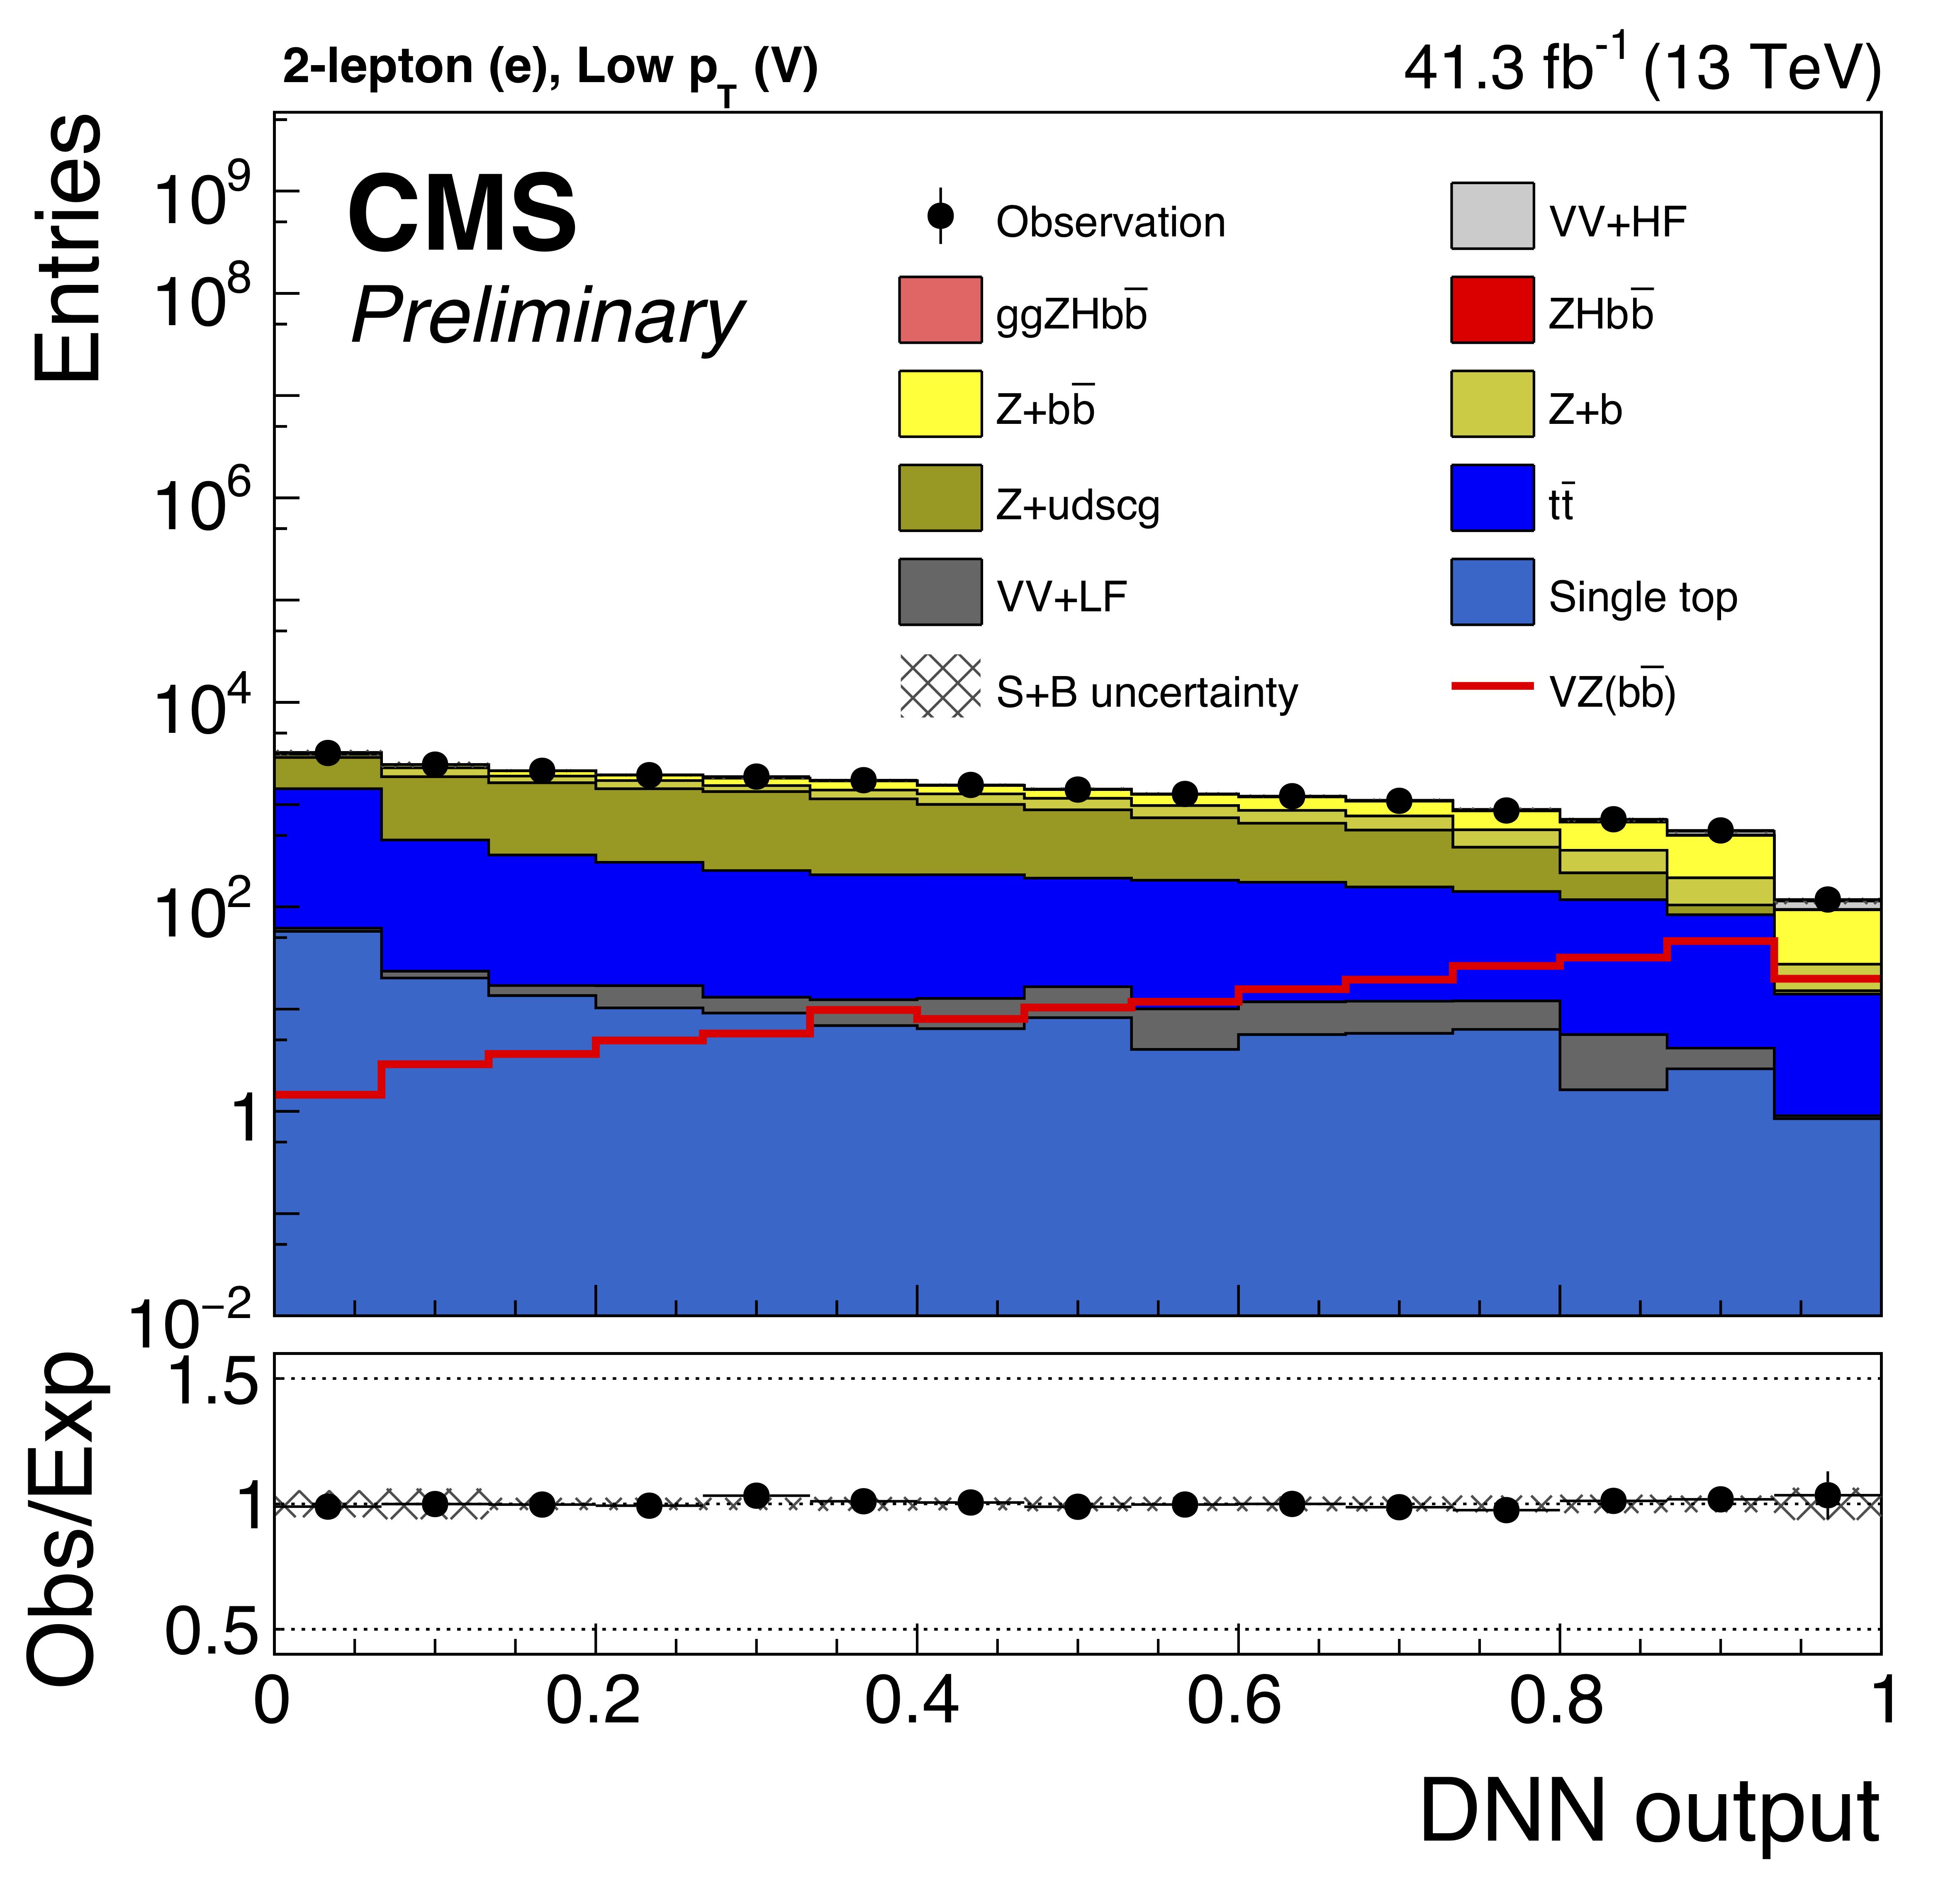
\includegraphics[width=0.285\linewidth]{images/SR_VZbb/vhbb_Zee_2_13TeV2017_shapes_postfit_logy}} \qquad
    \subfigure [] {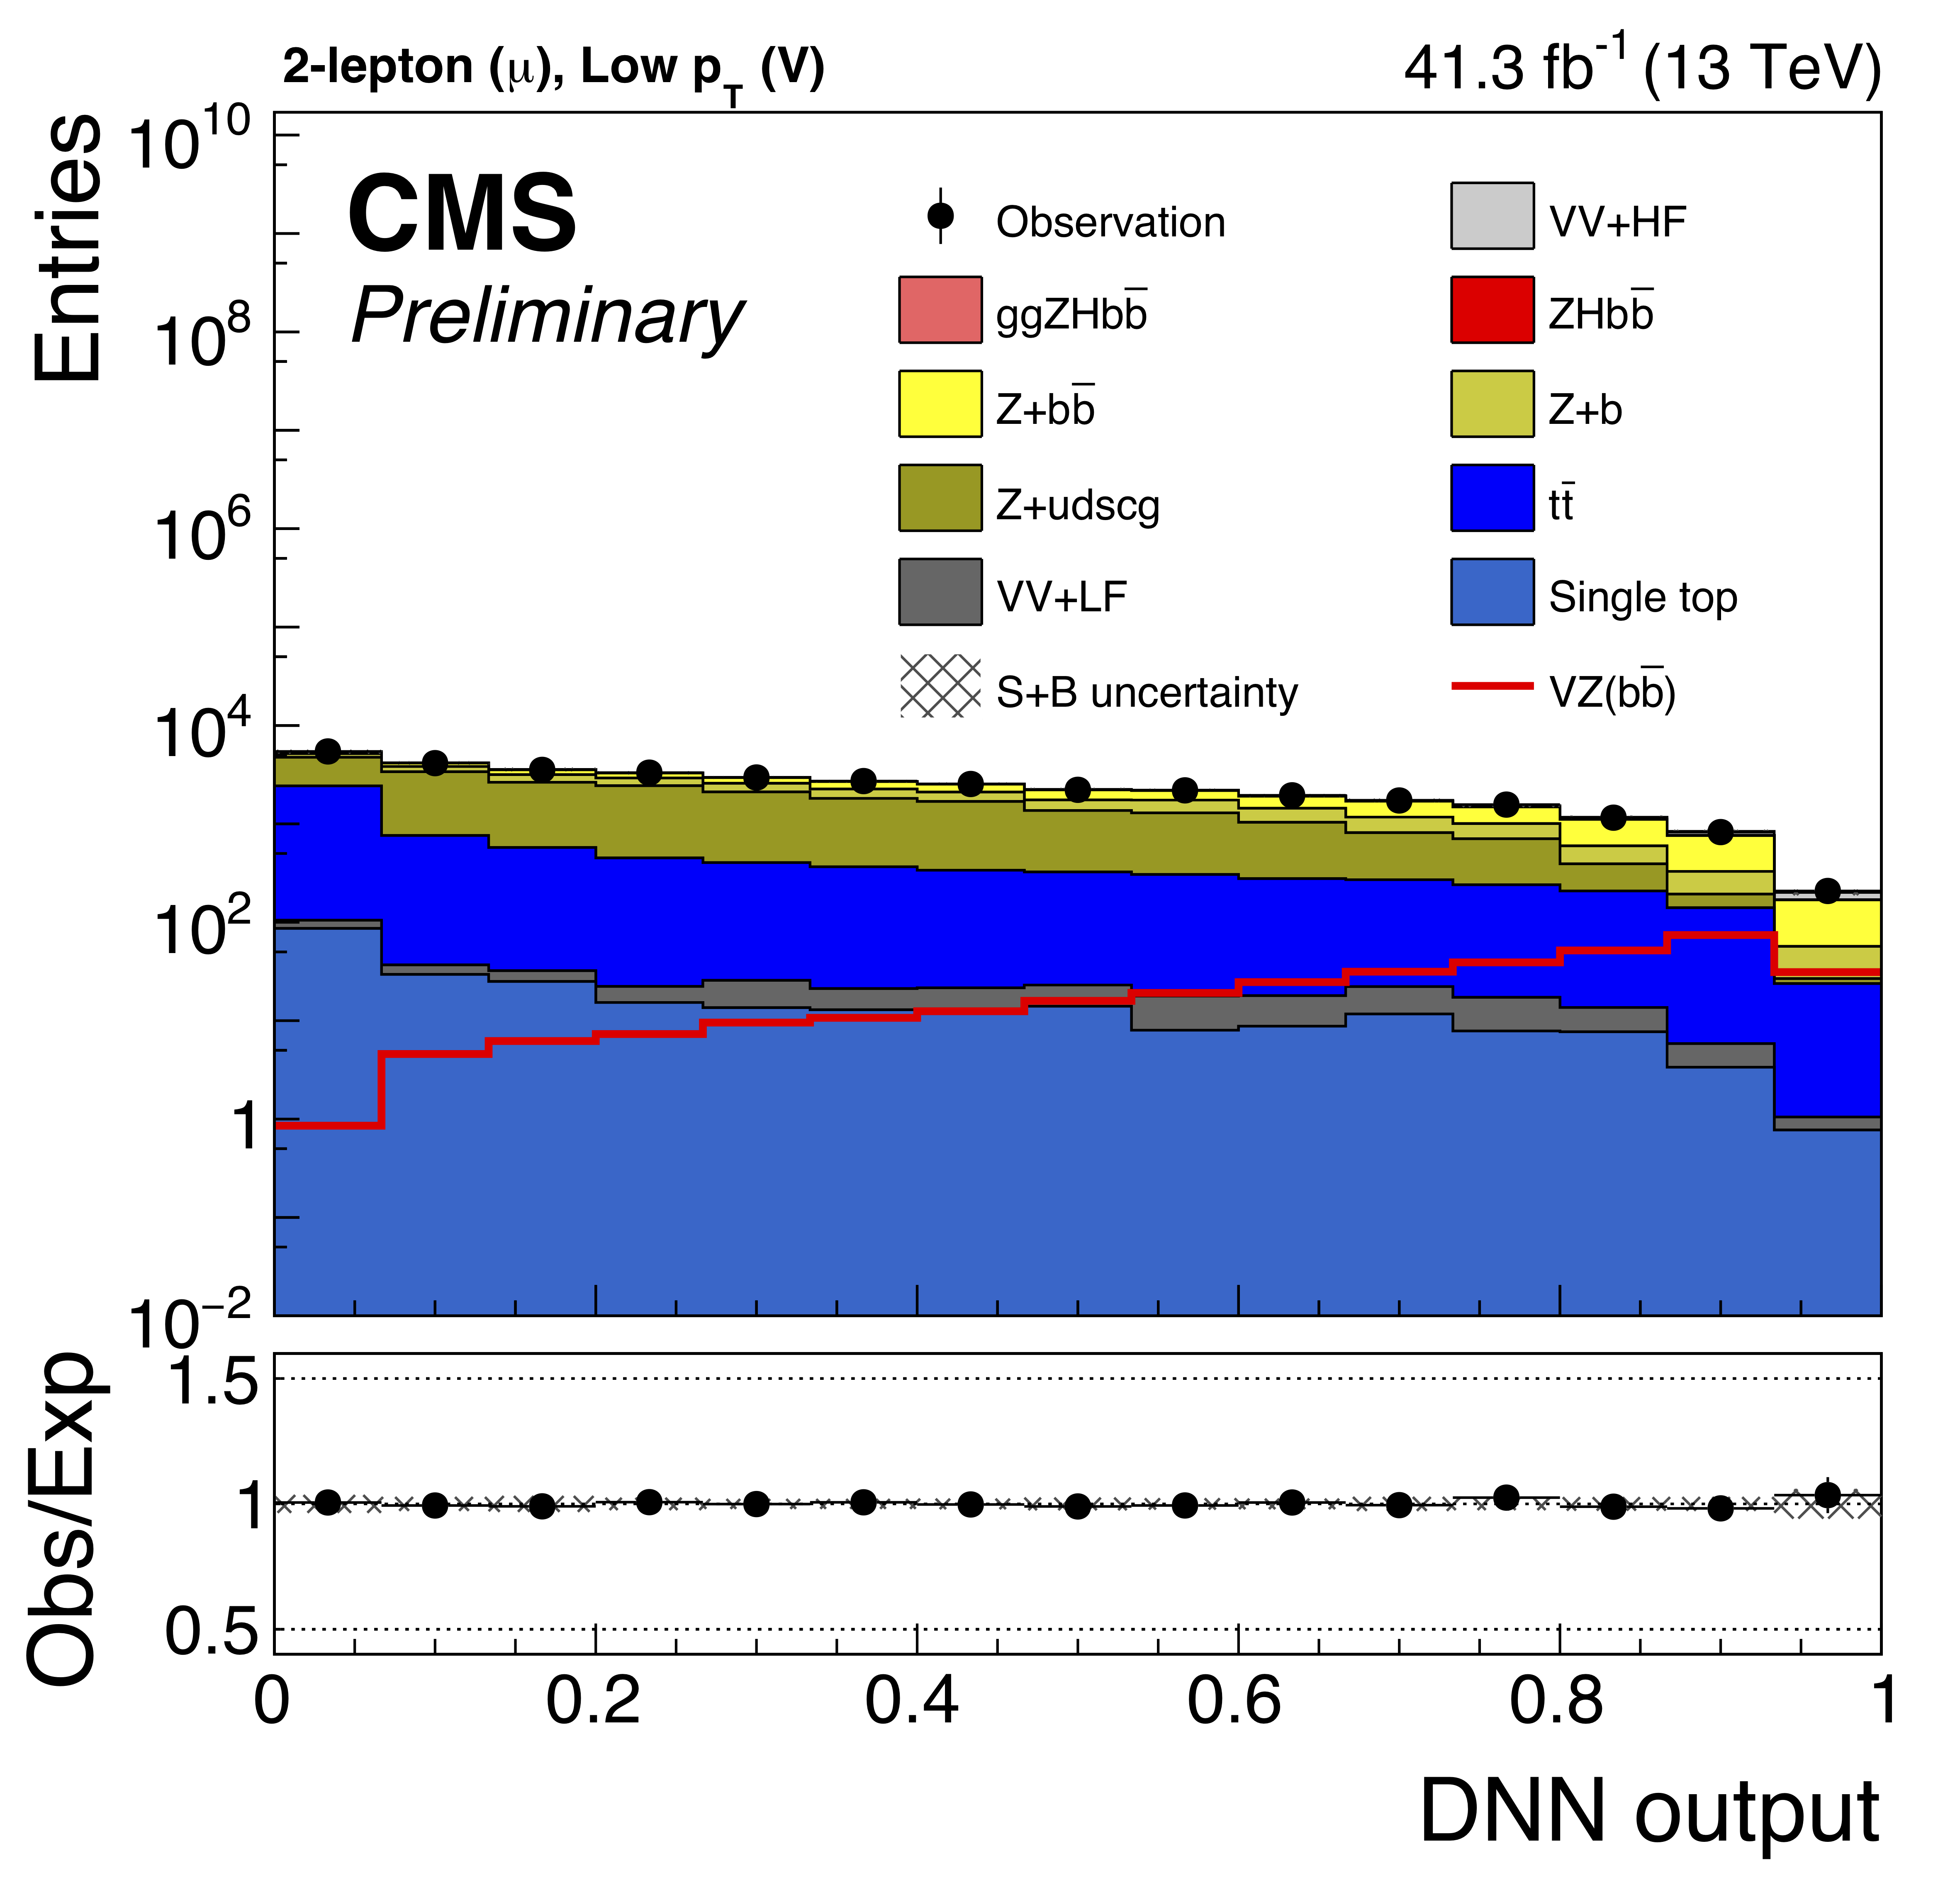
\includegraphics[width=0.285\linewidth]{images/SR_VZbb/vhbb_Zmm_2_13TeV2017_shapes_postfit_logy}} \qquad
  }
  \mbox{
    \subfigure [] {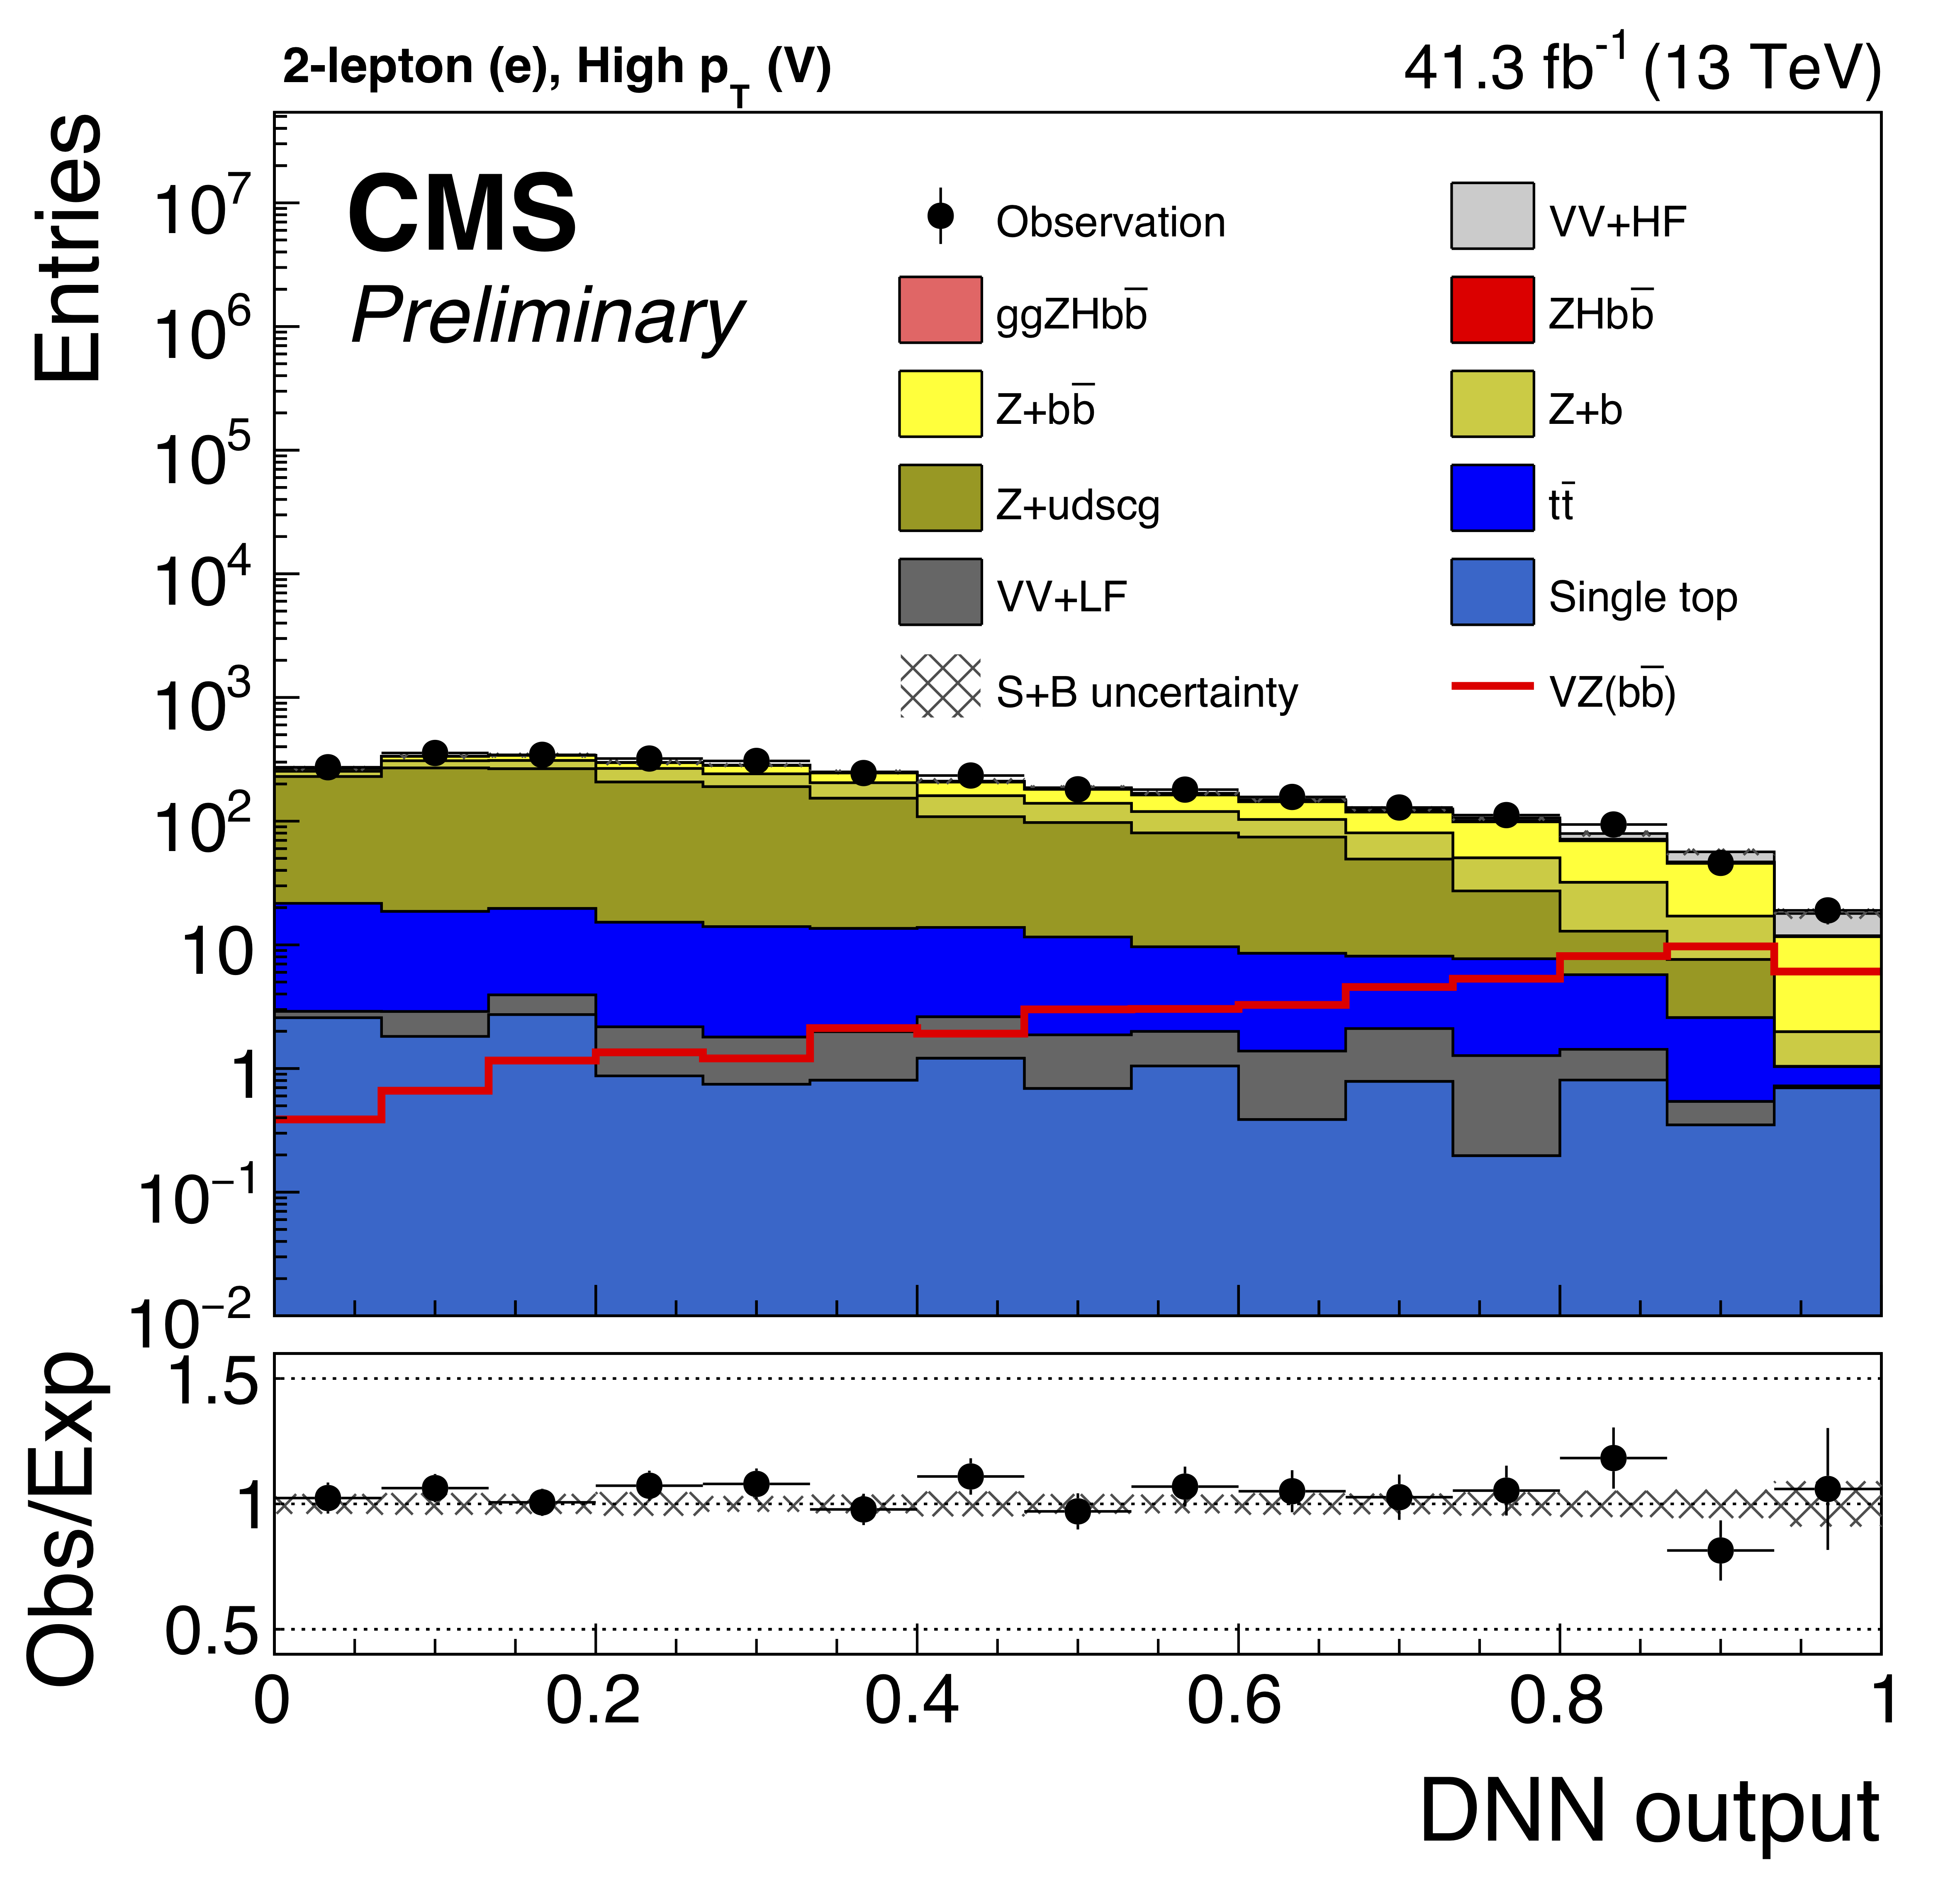
\includegraphics[width=0.285\linewidth]{images/SR_VZbb/vhbb_Zee_1_13TeV2017_shapes_postfit_logy}} \qquad
    \subfigure [] {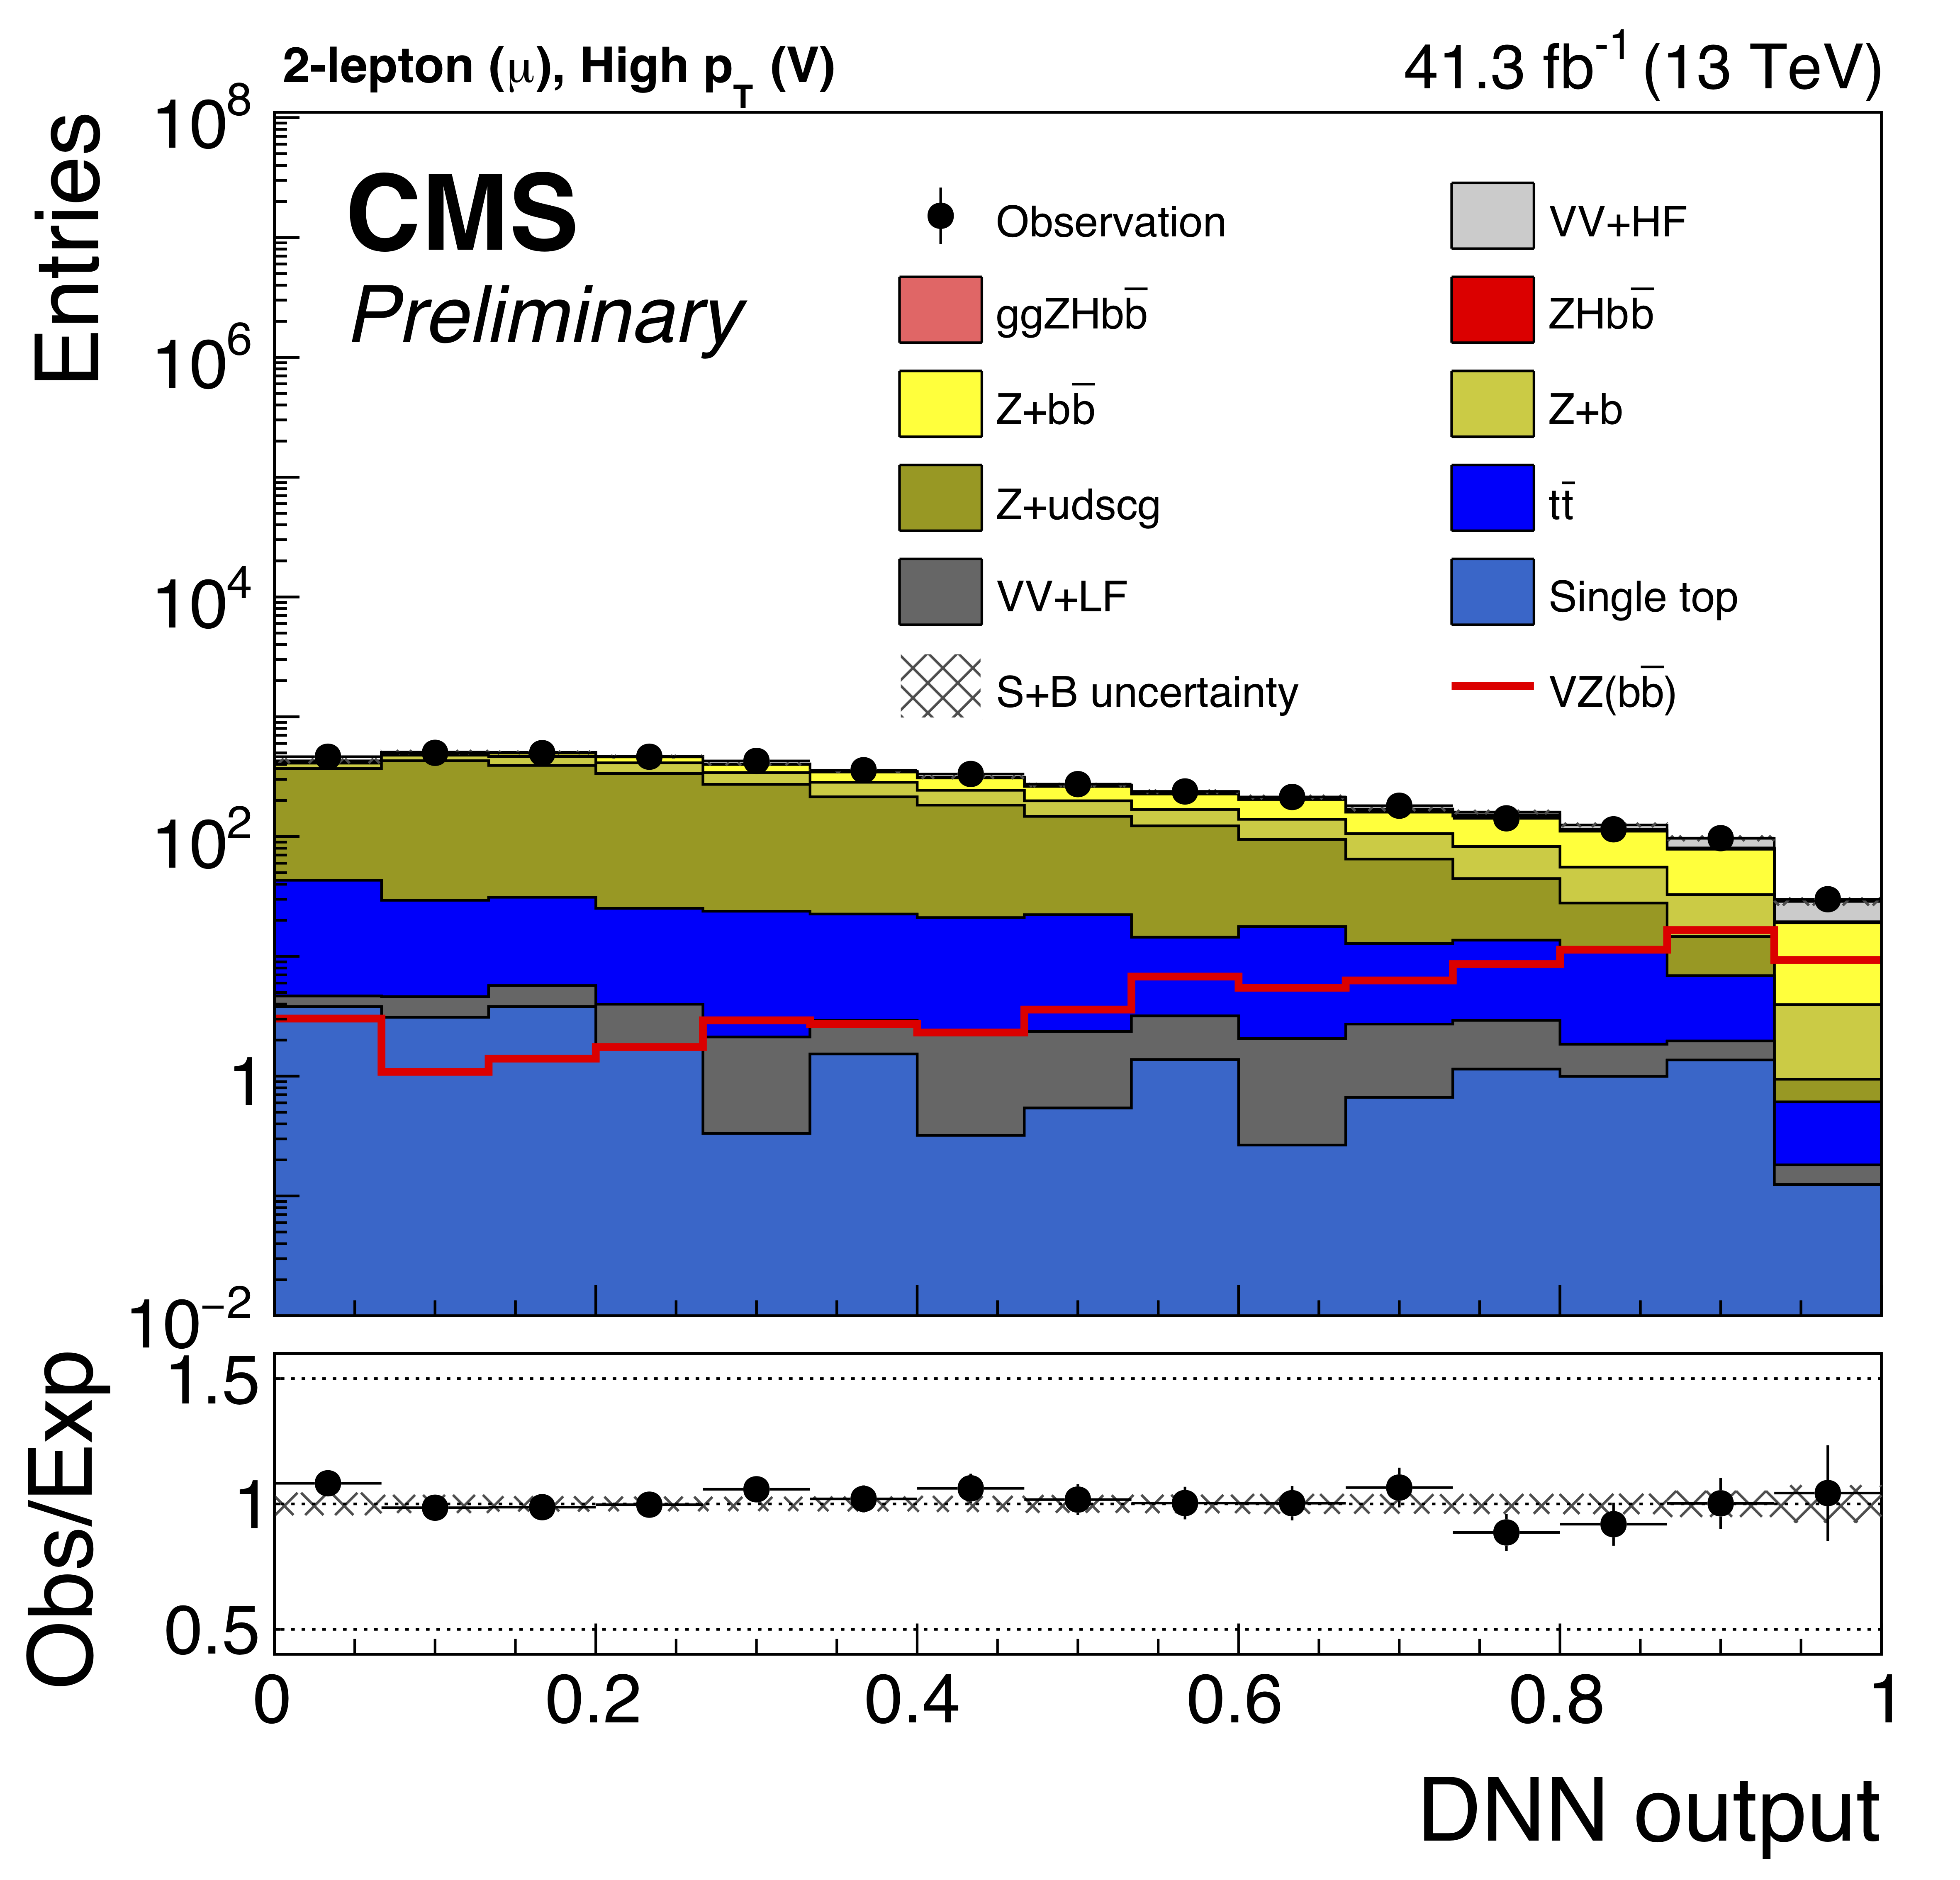
\includegraphics[width=0.285\linewidth]{images/SR_VZbb/vhbb_Zmm_1_13TeV2017_shapes_postfit_logy}} \qquad
  }
  \mbox{
    \subfigure [] {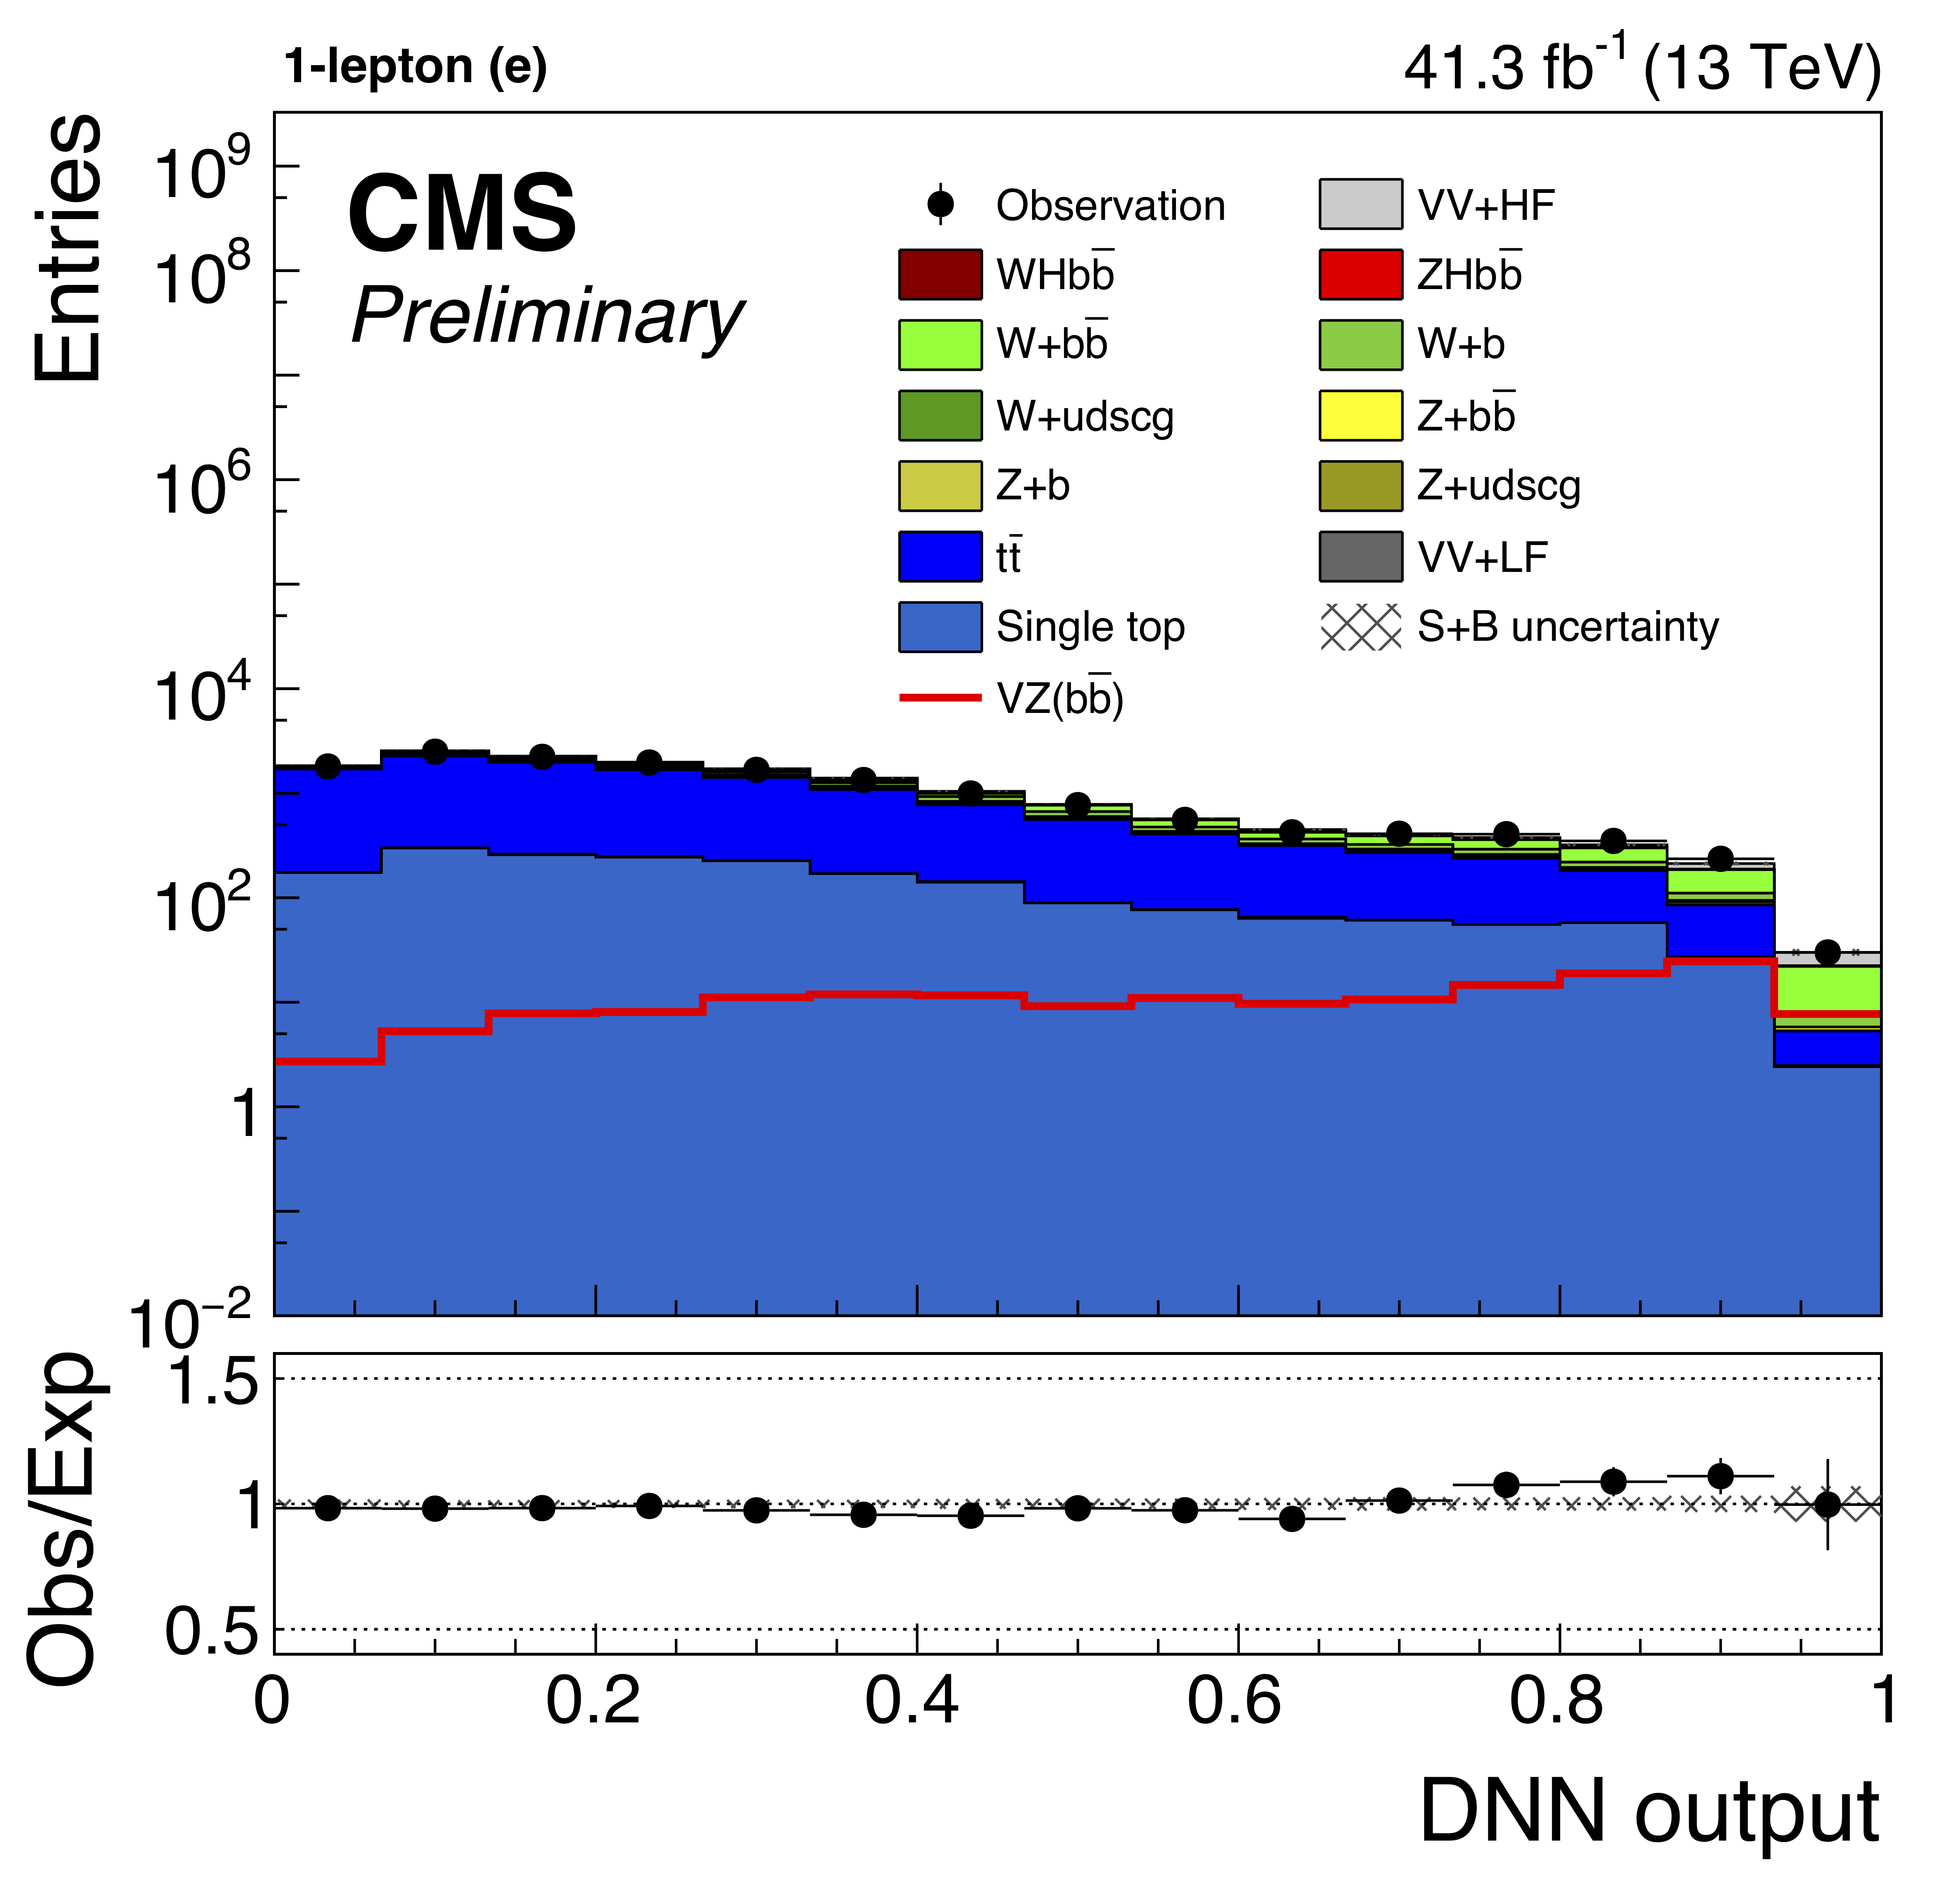
\includegraphics[width=0.285\linewidth]{images/SR_VZbb/vhbb_Wen_1_13TeV2017_shapes_postfit_logy}} \qquad
    \subfigure [] {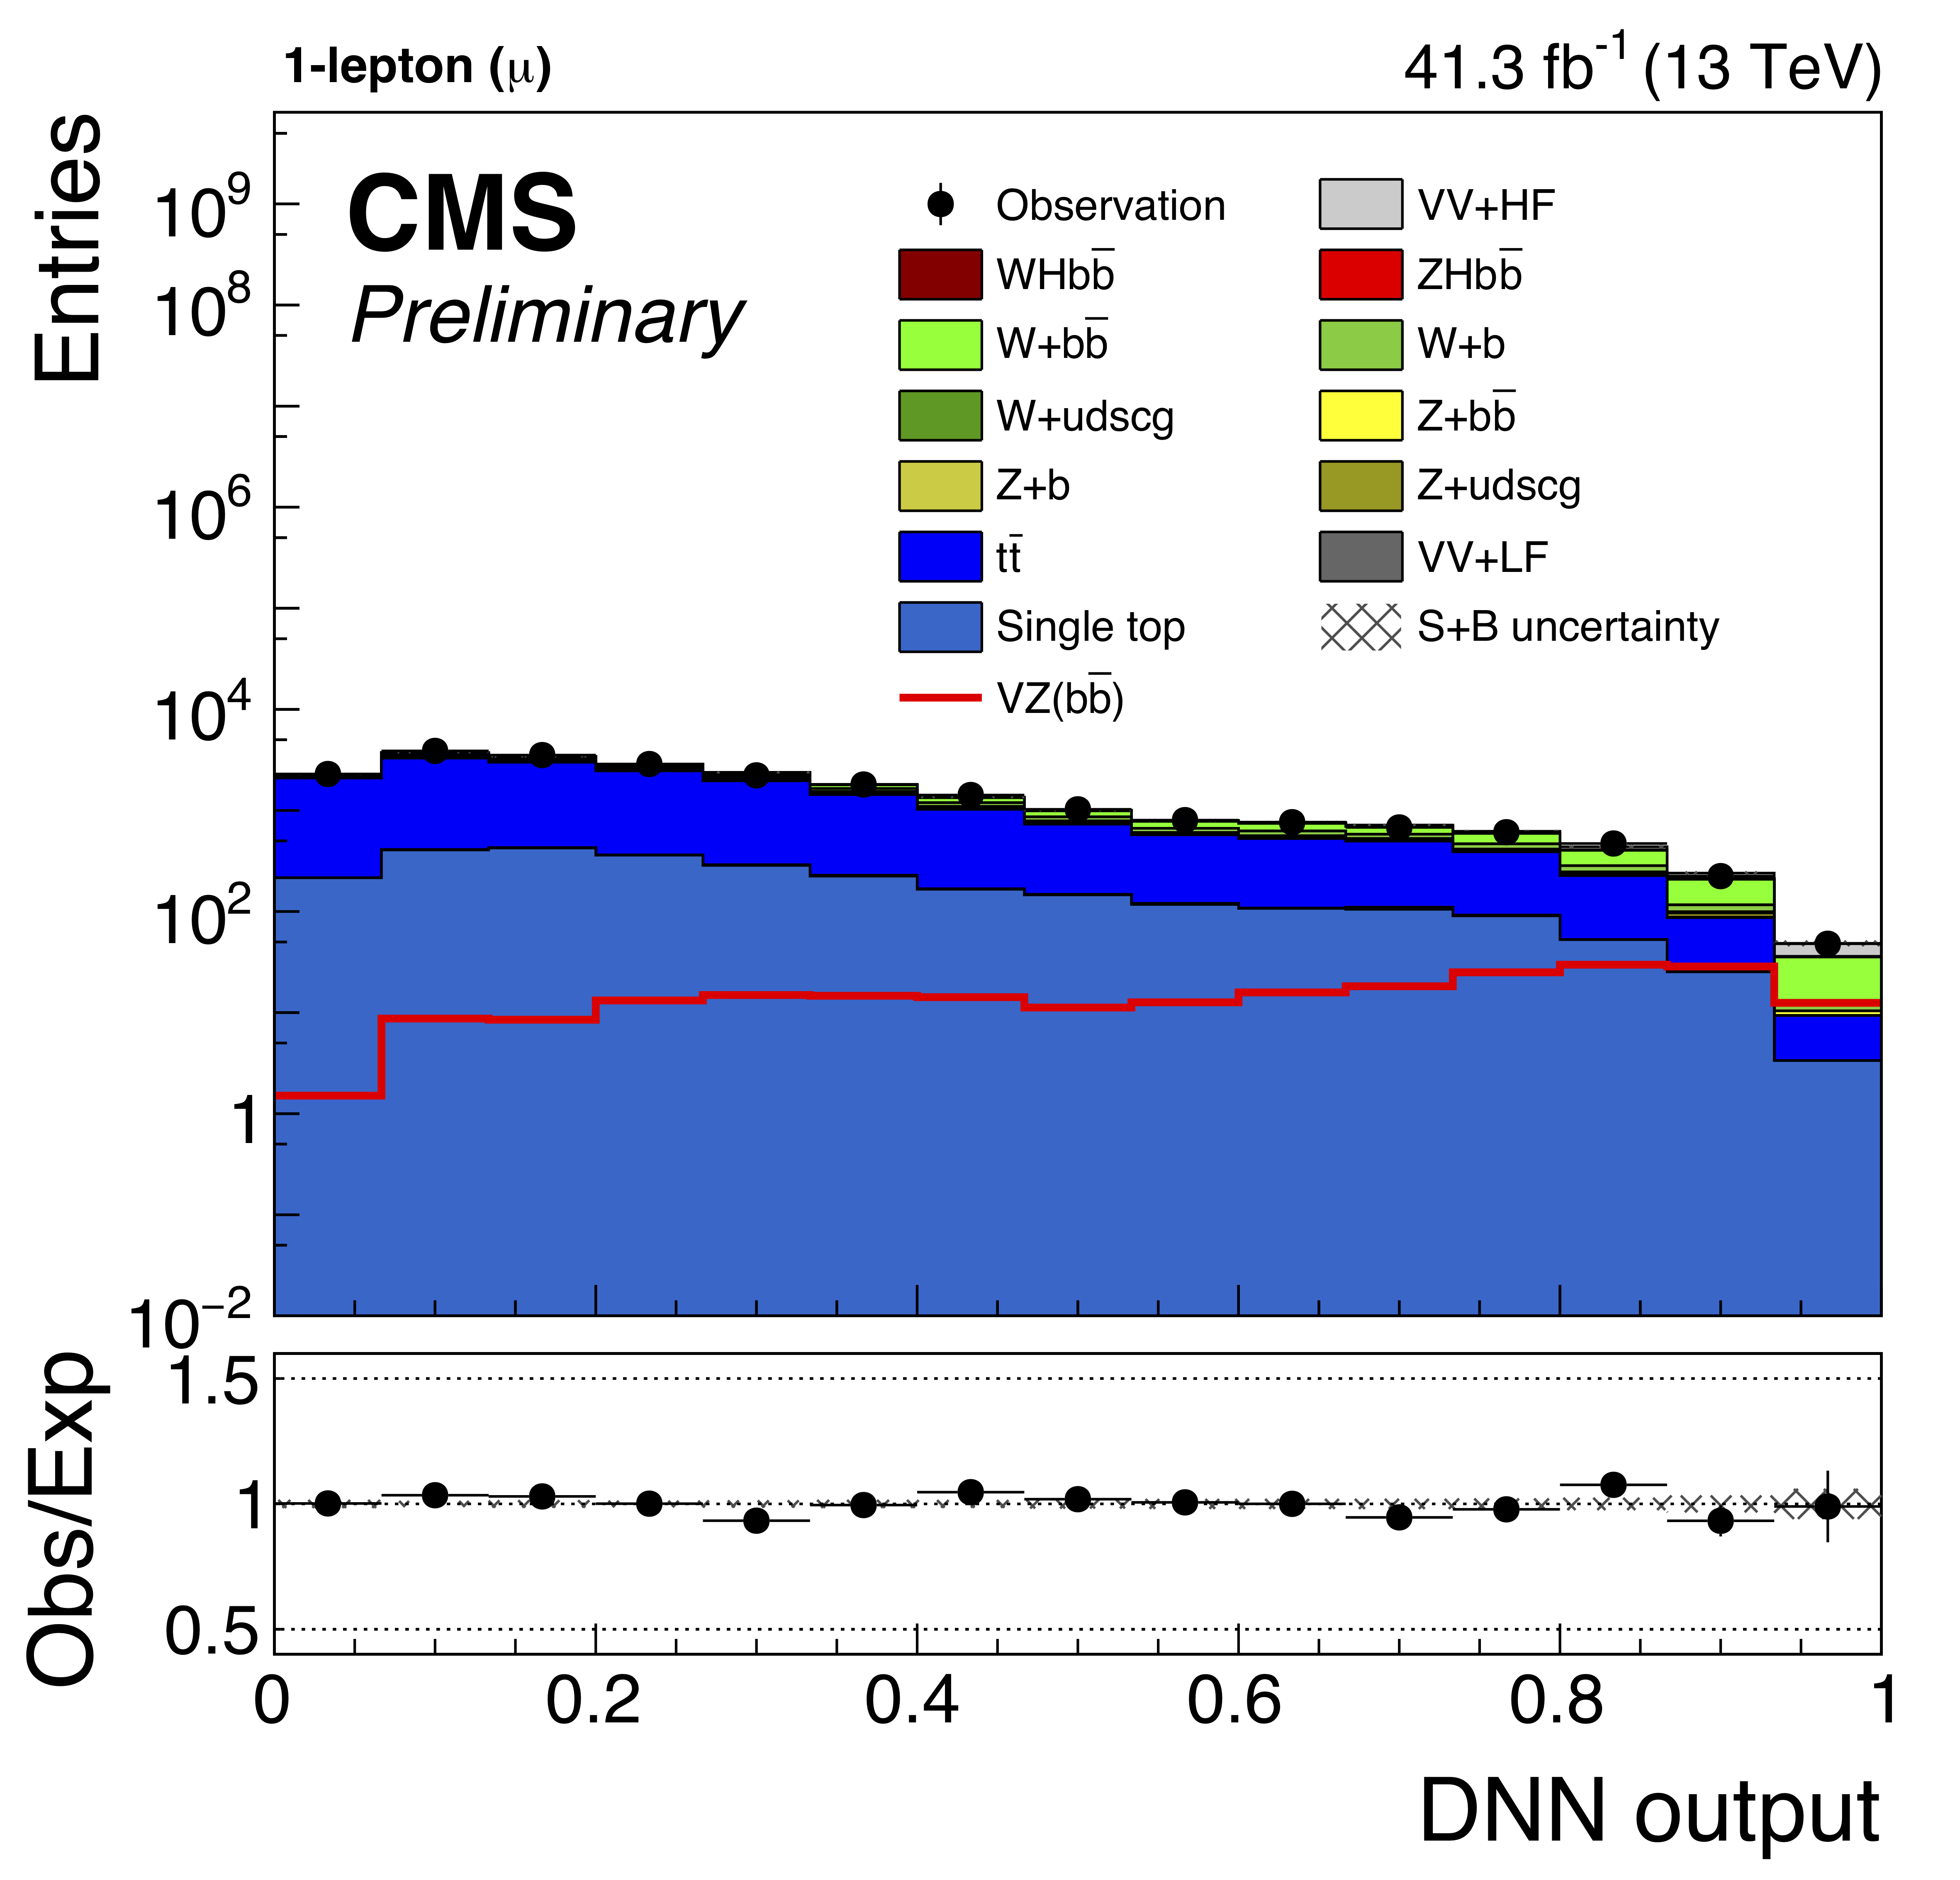
\includegraphics[width=0.285\linewidth]{images/SR_VZbb/vhbb_Wmn_1_13TeV2017_shapes_postfit_logy}} \qquad
  }
  \mbox{
    \subfigure [] {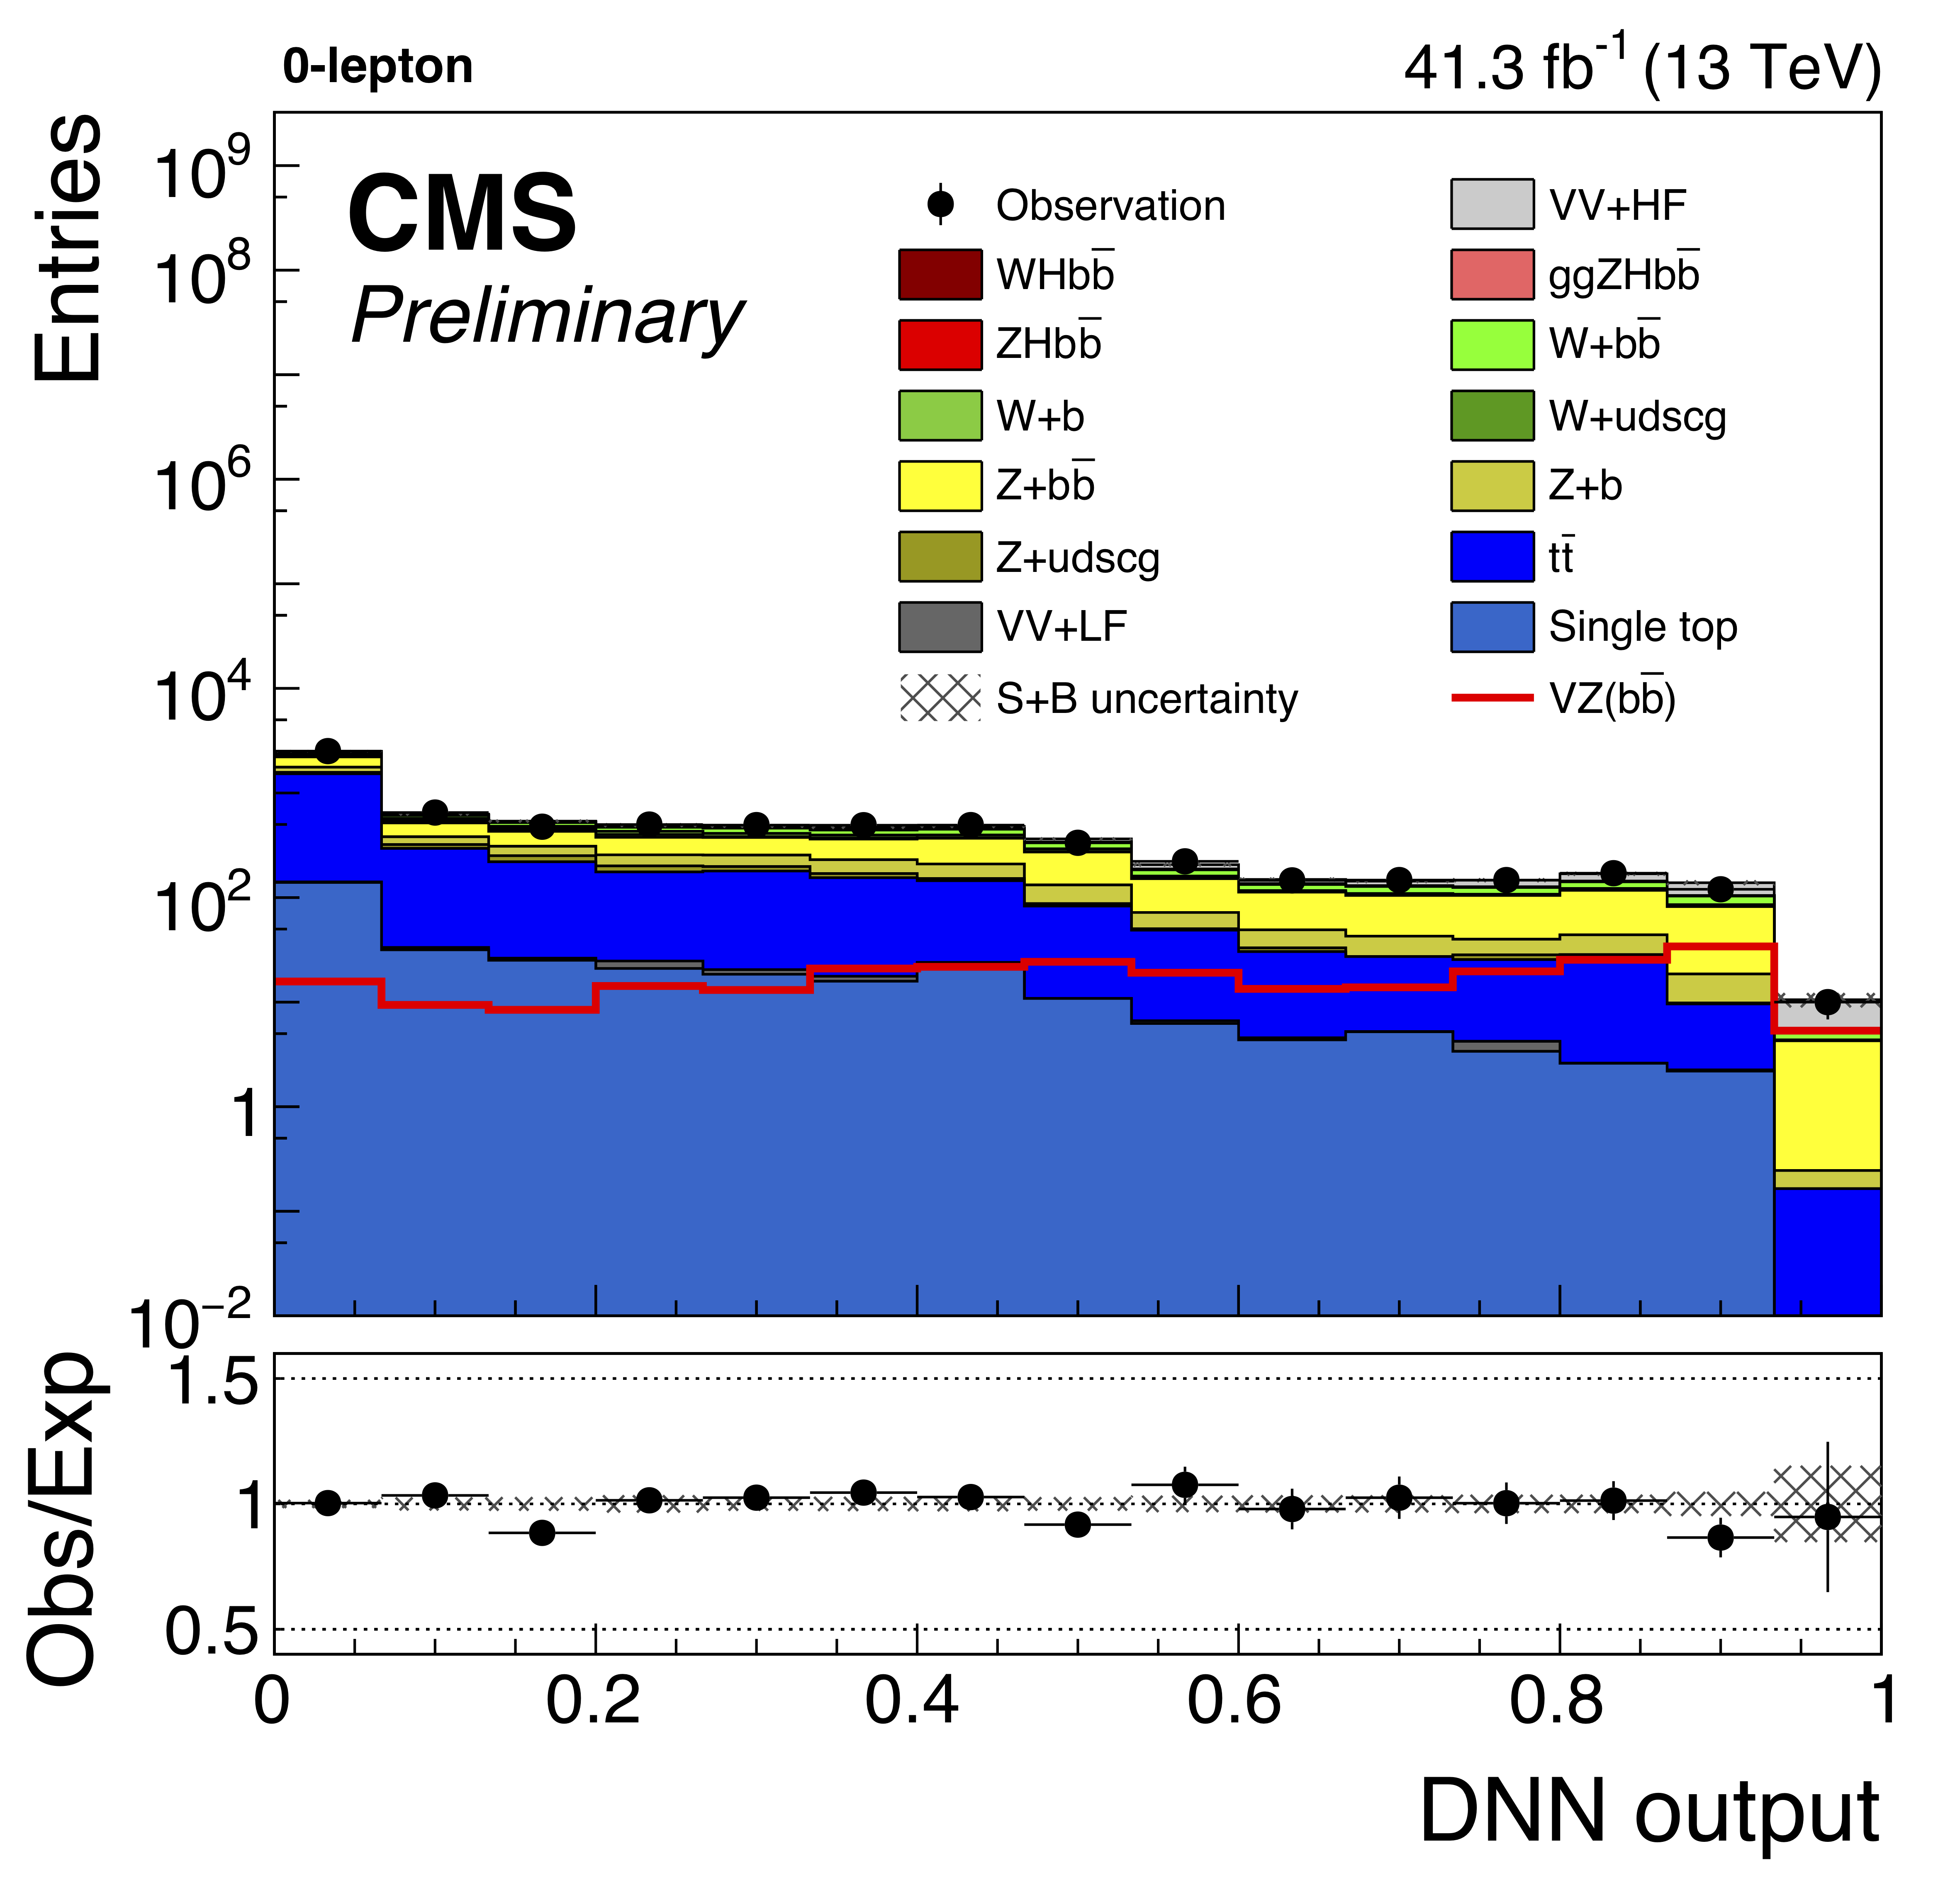
\includegraphics[width=0.285\linewidth]{images/SR_VZbb/vhbb_Znn_1_13TeV2017_shapes_postfit_logy}}
  }
  \caption[\VZbb\ Signal Region Distributions]{The post-fit \VZbb\ multivariate discriminant distributions of the A) low \pT(\bosV) \ZeeH; B) low \pT(\bosV) \ZmmH; C) high \pT(\bosV) \ZeeH; D) high \pT(\bosV) \ZmmH; E) \WenH; F) \WmnH; and G) \ZnnH\ channels.}
  \label{fig:SRVZbb}
\end{figure}

\begin{figure}[htbp]
  \centering
    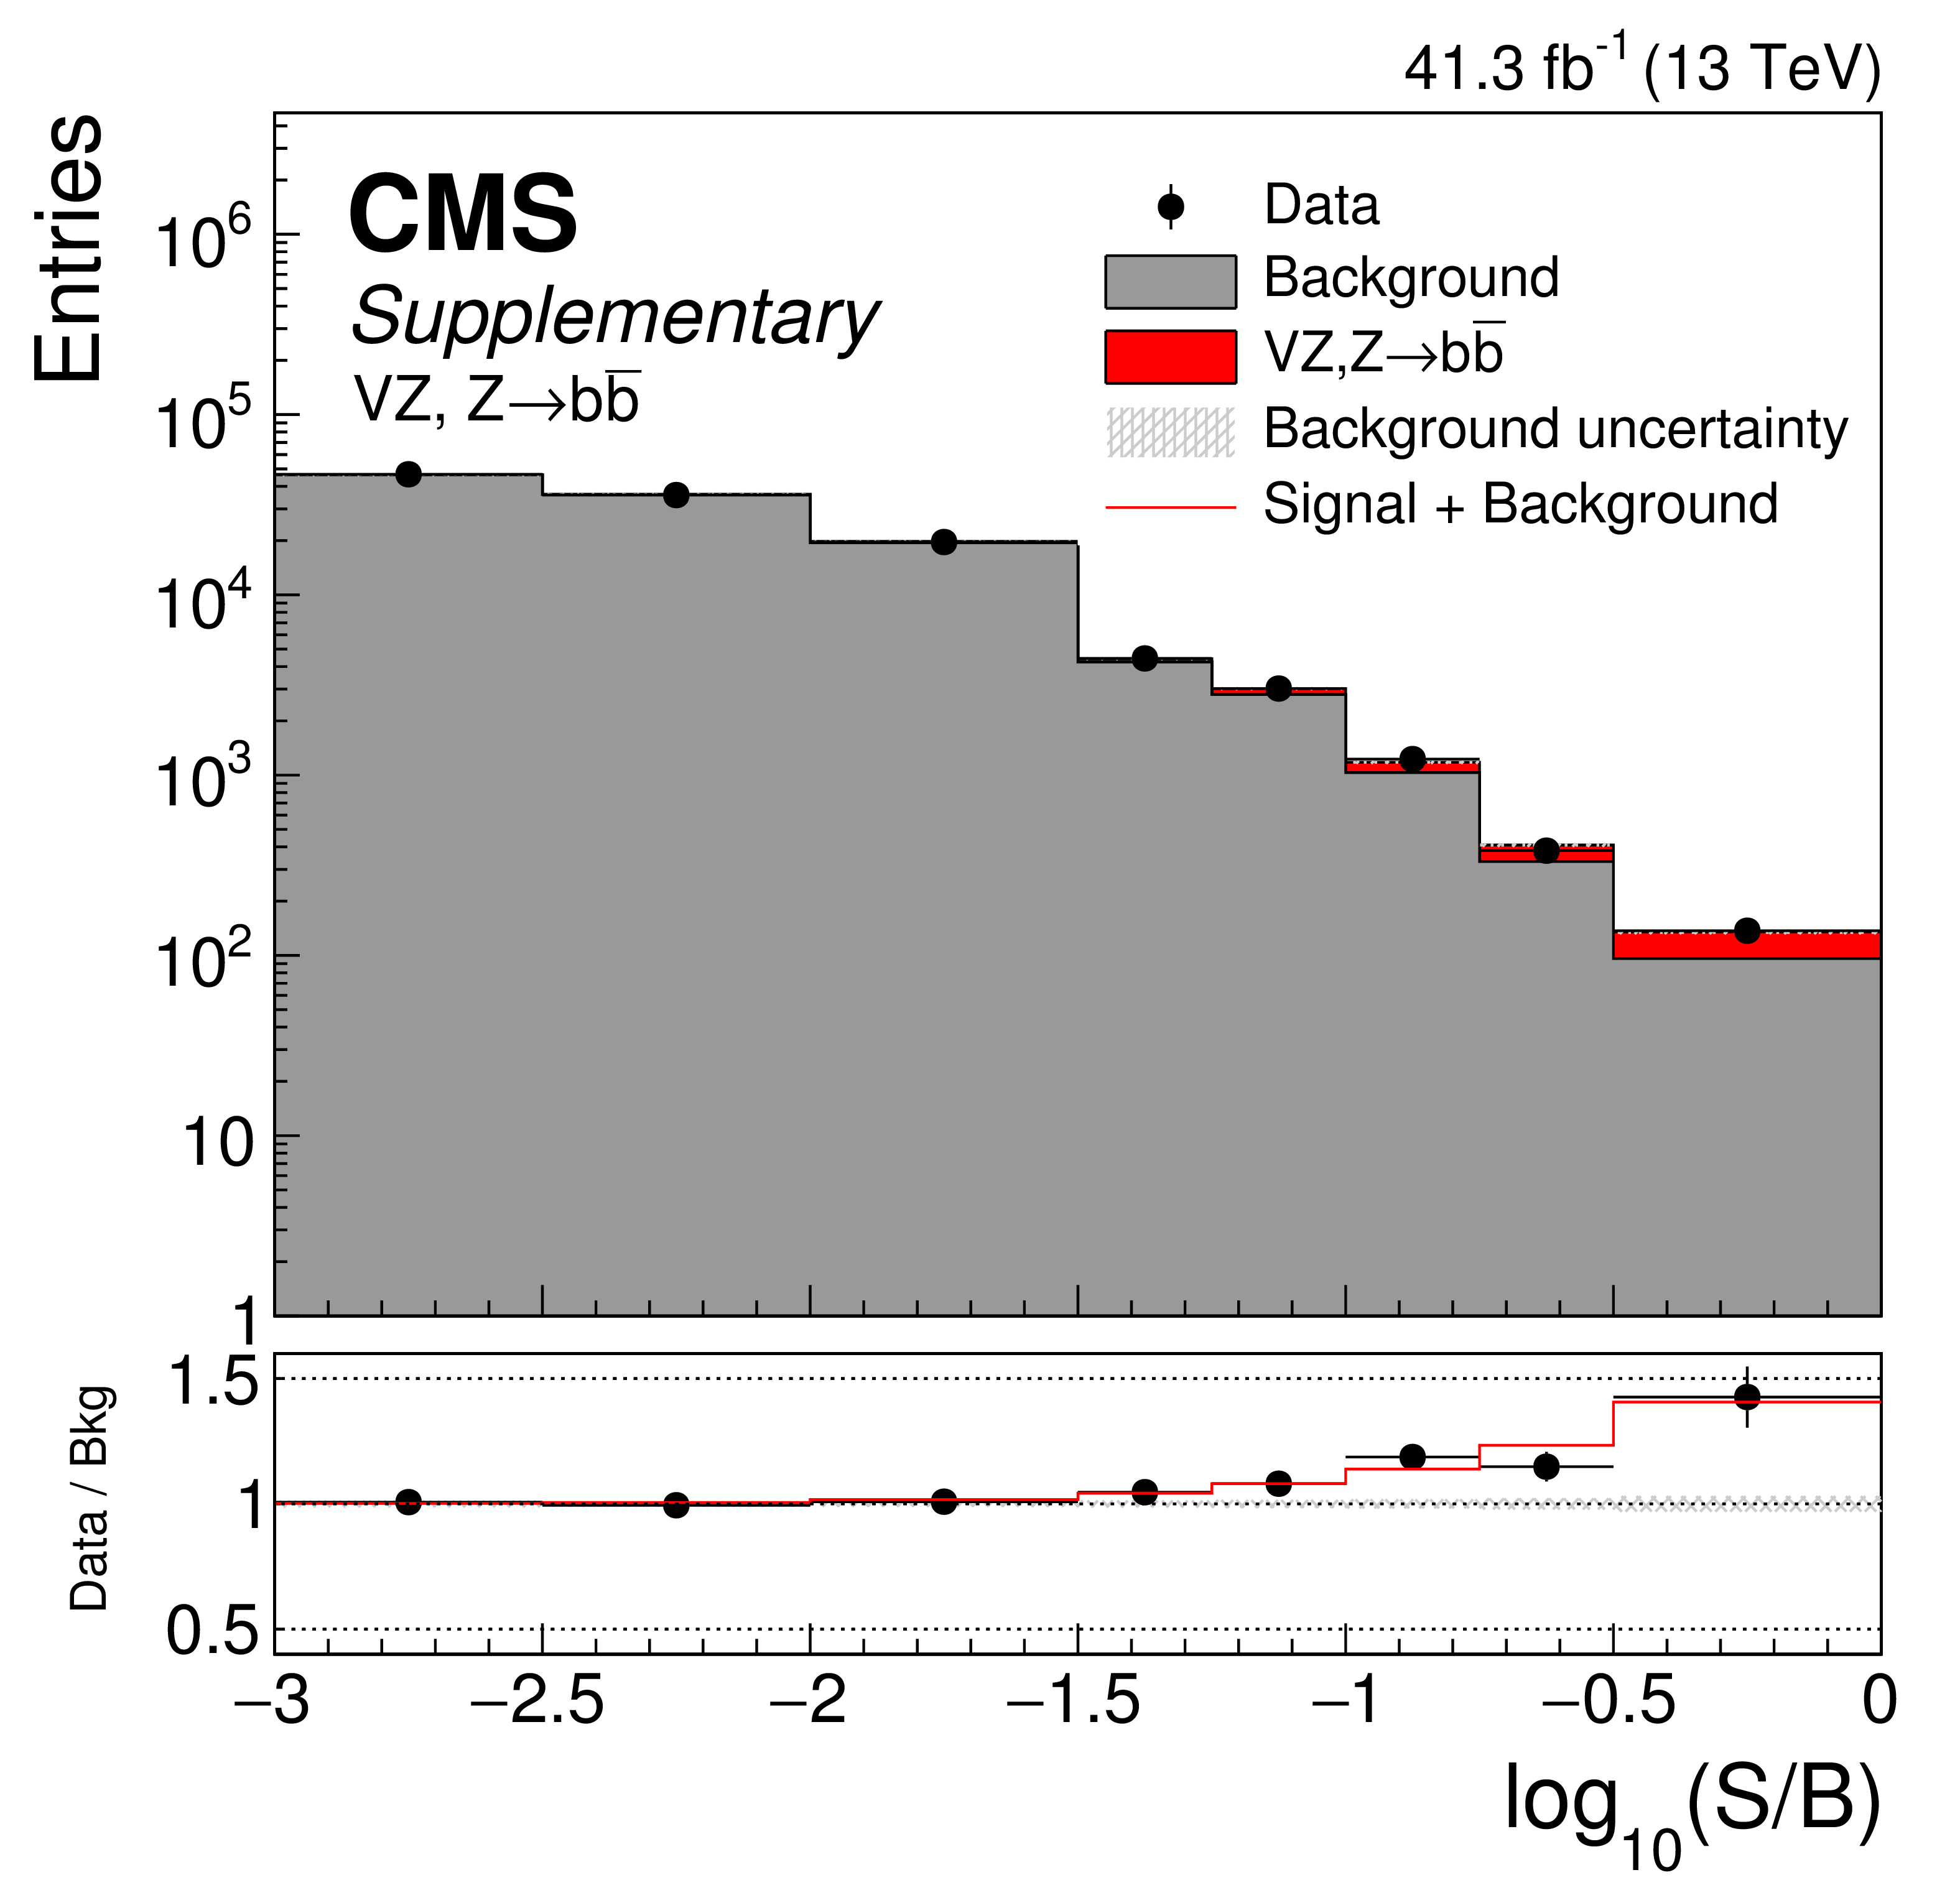
\includegraphics[width=3.5in]{images/CMS-HIG-18-016_Figure-aux_009}
    \caption[\VZbb\ Combined Signal Region Distribution]{The post-fit multivariate discriminant distributions of signal, background, and data event yields combined for all \VZbb\ channels and sorted into bins of similar signal-to-background ratio. The \VZbb\ signal contribution (red) has been stacked above the sum of all background yields (gray). The bottom panel shows the data to background ratio (black points) and the sum of signal and background contributions divided by the background yield (red line).}
    \label{fig:SBVZbb}
\end{figure}

\begin{figure}[htbp]
  \centering
    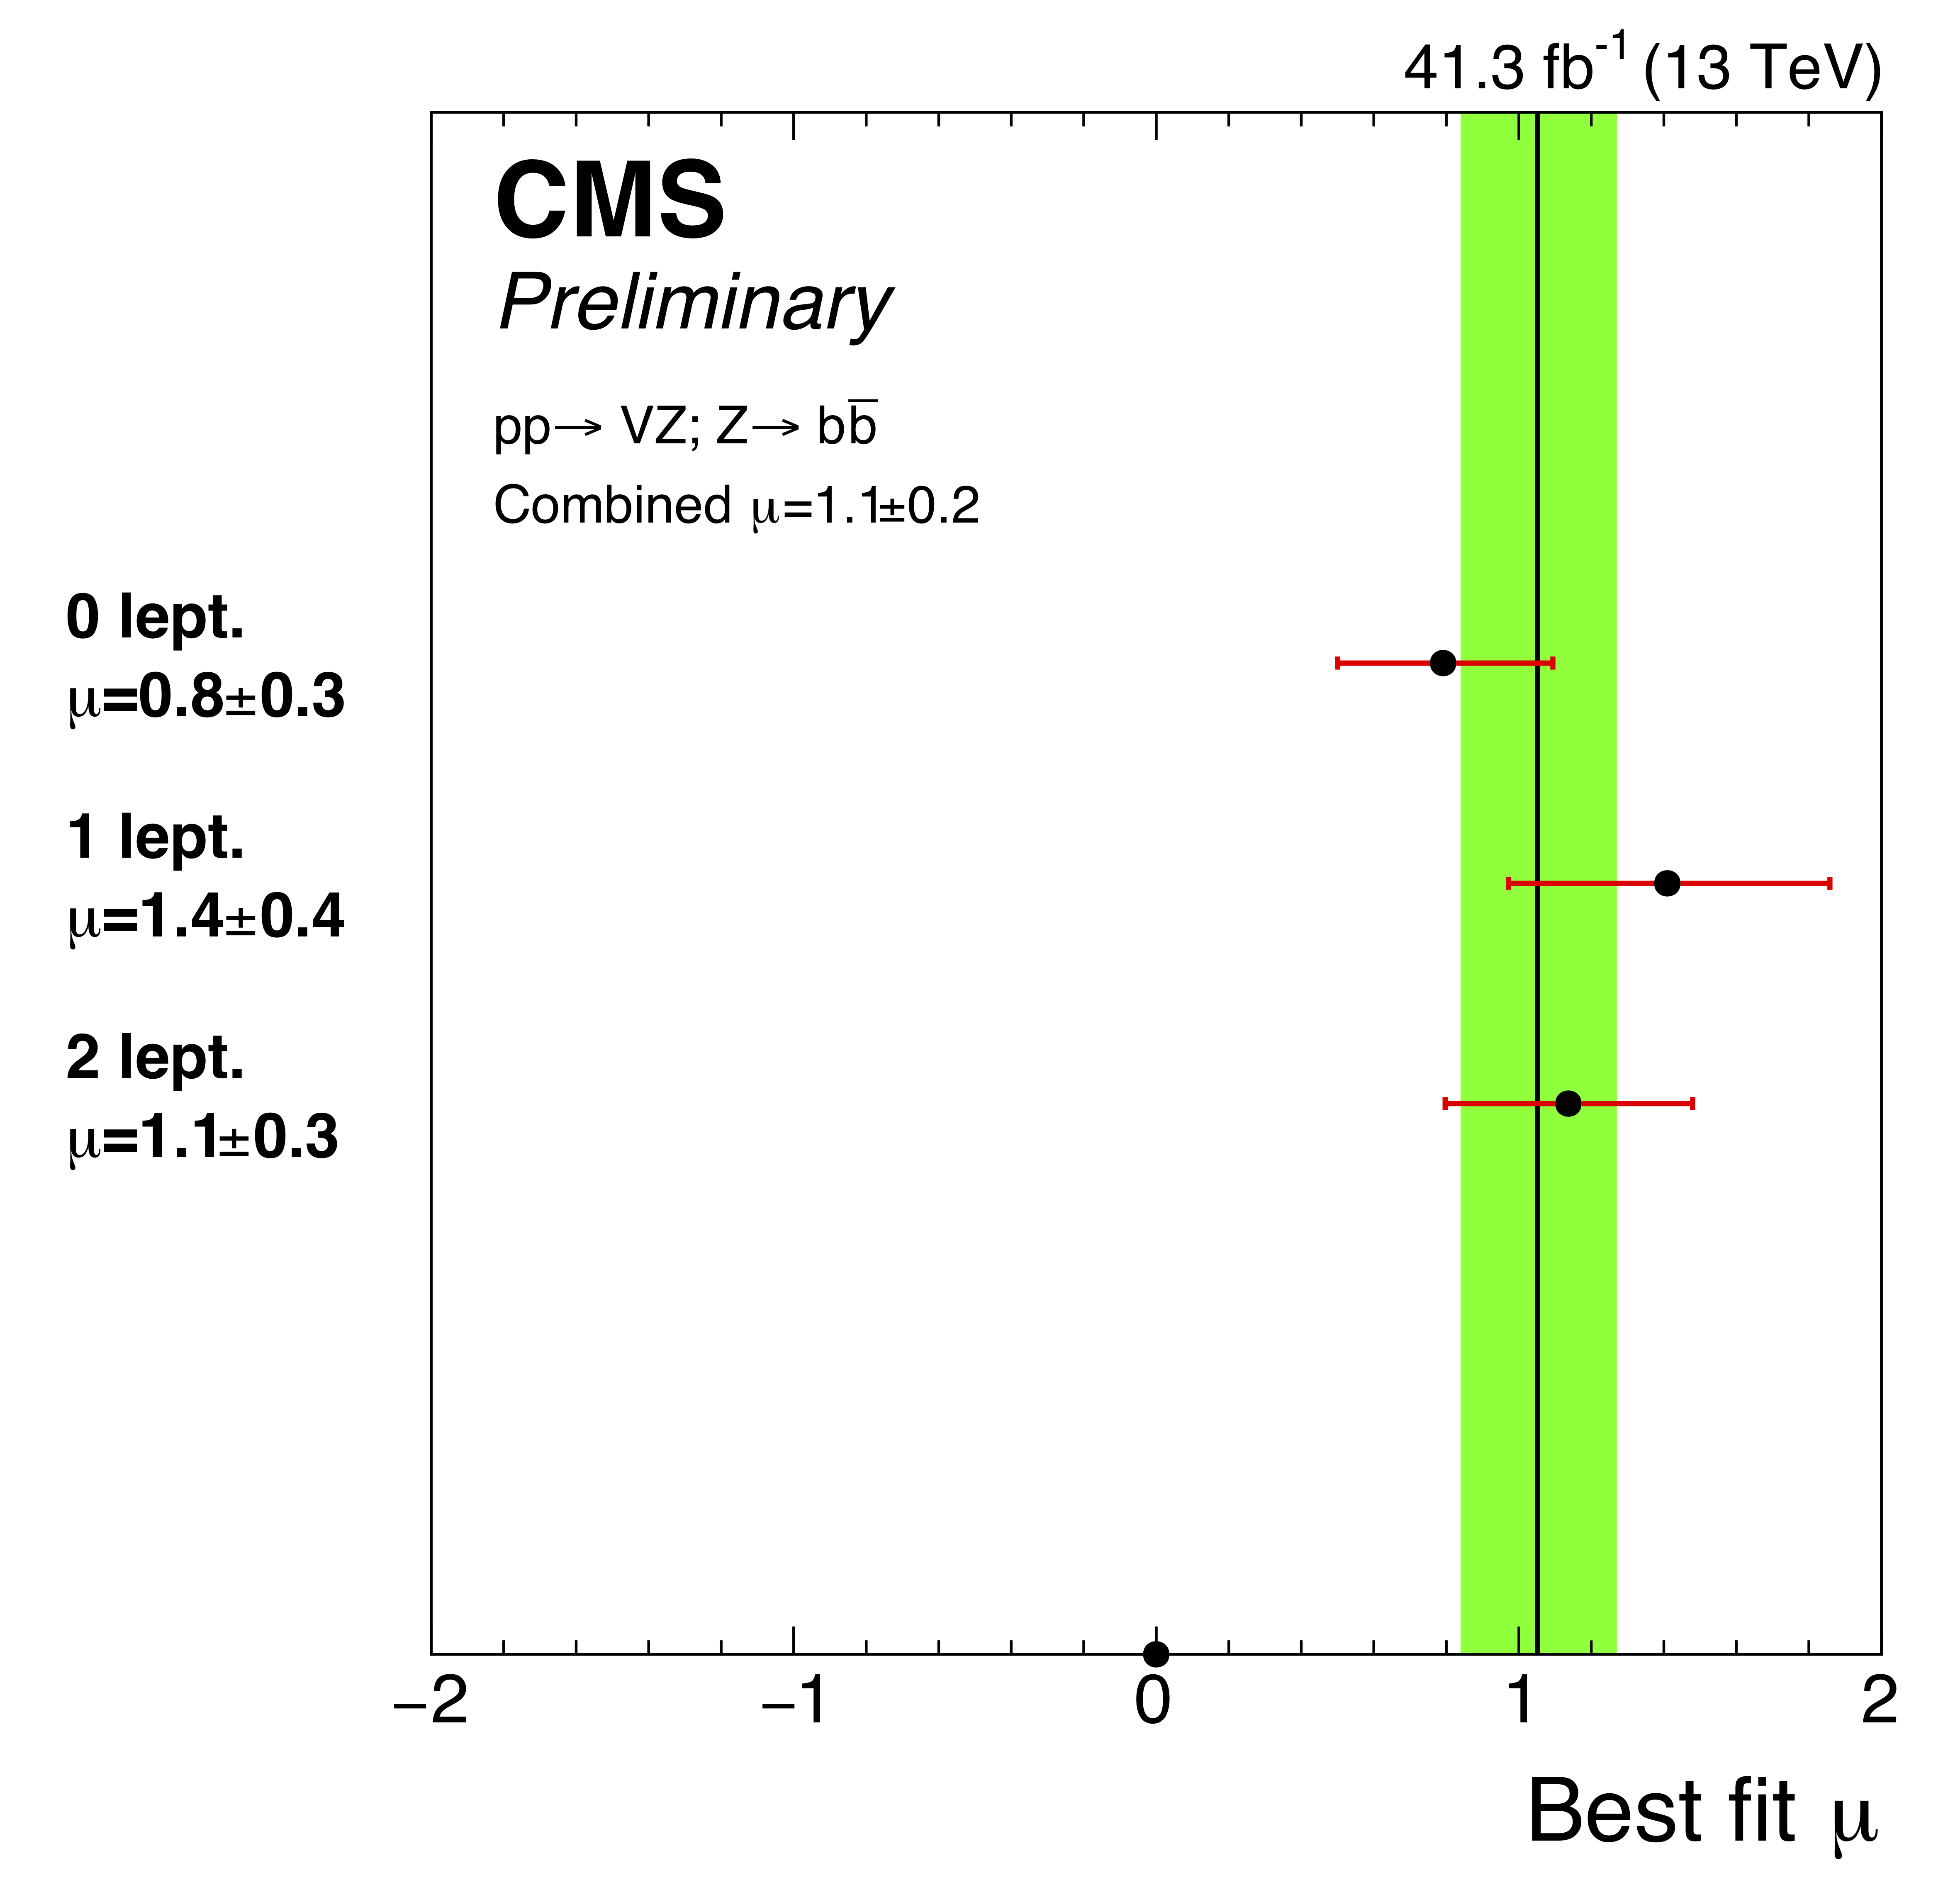
\includegraphics[width=3.5in]{images/MuVZbb}
    \caption[\VZbb\ Analysis Signal Strengths]{The best fit signal strengths and their uncertainties for each of the channels of the \VZbb\ cross-check analysis.}
    \label{fig:MuVZbb}
\end{figure}

\section{Dijet Invariant Mass Analysis}

The optimal massless DNN score values that divide the signal regions of each of the decay channels into four separate mass categories are listed in Table \ref{tbl:MjjVHbb}. The data to MC scale factors obtained by the maximum likelihood fit are shown in Table \ref{tbl:SFMjj}. The expected post-fit significance of the excess over the background prediction is $2.19\sigma$, while the observed significance is $1.33\sigma$. The best fit signal strength is $\mu = 0.59_{-0.45}^{+0.45}$ for all channels combined. By combining the dijet invariant mass distributions of all channels with weight $S/(S+B)$, where $S$ is the post-fit \VHbb signal yield and $B$ is the post-fit total background yield specific to each channel, and then subtracting the contributions of all background processes except for \VZbb, the capability of resolving the \VHbb\ mass peak against the \VZbb\ mass peak without a multivariate analysis is shown in Figure \ref{fig:WeightedMjj}.

\begin{table}[htbp]
  \caption[Dijet Invariant Mass Analysis Categories]{The massless DNN scores which define the boundaries of the four dijet invariant mass categories of each \VHbb\ channel.}
  \label{tbl:MjjVHbb}
  \begin{tabularx}{6.5in}{XX}
    \hline
    Channel                & Mass Category Boundaries          \\
    \hline
    \ZnnH                  & [0.00, 0.558, 0.768, 0.838, 1.00] \\
    \WlnH                  & [0.00, 0.550, 0.856, 0.941, 1.00] \\
    \ZllH, Low \pT(\bosV)  & [0.00, 0.662, 0.875, 0.927, 1.00] \\
    \ZllH, High \pT(\bosV) & [0.00, 0.486, 0.836, 0.899, 1.00] \\
    \hline
  \end{tabularx}
\end{table}

\begin{table}[htbp]
  \caption[Dijet Invariant Mass Analysis Scale Factors]{The data to Monte-Carlo scale factors obtained by the simultaneous maximum likelihood fit over all \VHbb\ channels for the dijet invariant mass analysis. The errors include both statistical and systematic uncertainties.}
  \label{tbl:SFMjj}
  \begin{tabularx}{6.5in}{lXXll}
    \hline
    Process       & \ZnnH           & \WlnH           & \ZllH, Low \pT(\bosV) & \ZllH, High \pT(\bosV) \\
    \hline
    \Wlight       & $1.02 \pm 0.07$ & $1.02 \pm 0.07$ & -                     & -                      \\
    \Wb           & $1.82 \pm 0.14$ & $1.82 \pm 0.14$ & -                     & -                      \\
    \Wbb          & $2.05 \pm 0.22$ & $2.05 \pm 0.22$ & -                     & -                      \\
    \Zlight       & $0.95 \pm 0.08$ & -               & $0.88 \pm 0.06$       & $0.81 \pm 0.05$        \\
    \Zb           & $1.16 \pm 0.16$ & -               & $0.99 \pm 0.13$       & $1.12 \pm 0.11$        \\
    \Zbb          & $1.00 \pm 0.08$ & -               & $0.72 \pm 0.06$       & $0.82 \pm 0.07$        \\
    \qrkt\qrktbar & $0.97 \pm 0.08$ & $0.90 \pm 0.07$ & $0.89 \pm 0.07$       & $0.88 \pm 0.07$        \\
    \hline
  \end{tabularx}
\end{table}

\begin{figure}[htbp]
  \centering
    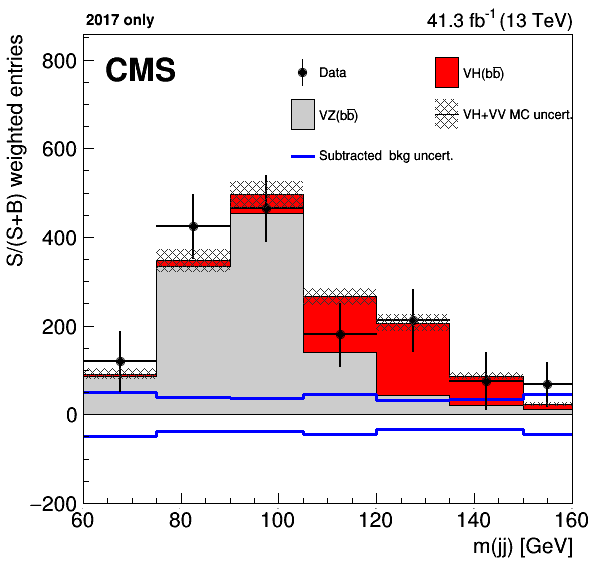
\includegraphics[width=3.5in]{images/only2017_shapesMjj1617_postfit}
    \caption[Combined Dijet Invariant Mass Distribution]{The dijet invariant mass distribution for events weighted by $S/(S+B)$ in all channels combined. The data (black) and the fitted \VHbb\ signal (red) and \VZbb\ background (gray) distributions are shown with all other fitted backgrounds subtracted. The vertical error bars represent the $1\sigma$ statistical uncertainty on the data before background subtraction, while the blue error band represents the $1\sigma$ total uncertainty on the signal and all background processes.}
    \label{fig:WeightedMjj}
\end{figure}

\section{\VHbb\ Analysis}

The data to MC scale factors obtained by the maximum likelihood fit are shown in Table \ref{tbl:SFVHbb} and show good agreement with those obtained by the \VZbb\ cross-check analysis. The post-fit multivariate discriminant distributions of each channel are shown individually in Figure \ref{fig:SRVHbb} and combined in Figure \ref{fig:SBVHbb}. The expected post-fit significance of the excess over the background prediction is $3.1\sigma$, while the observed significance is $3.3\sigma$. The best fit signal strength is $\mu = 1.08_{-0.33}^{+0.35}$ for all channels combined and the signal strengths of the individual channels, shown in Figure \ref{fig:MuVHbb}, are compatible with a $p$-value of 96\%. These results reestablish evidence for the \VHbb\ decay. The contributions of the major uncertainty sources are listed in Table \ref{tbl:UncVHbb} and decomposed into four groups: theory, size of simulated samples, experimental, and statistical. For each major source of uncertainty, the largest individual subcomponents are also listed.

\begin{table}[htbp]
  \caption[\VHbb\ Analysis Scale Factors]{The data to Monte-Carlo scale factors obtained by the simultaneous maximum likelihood fit over all \VHbb\ channels. The errors include both statistical and systematic uncertainties.}
  \label{tbl:SFVHbb}
  \begin{tabularx}{6.5in}{lXXll}
    \hline
    Process       & \ZnnH           & \WlnH           & \ZllH, Low \pT(\bosV) & \ZllH, High \pT(\bosV) \\
    \hline
    \Wlight       & $1.04 \pm 0.07$ & $1.04 \pm 0.07$ & -                     & -                      \\
    \Wb           & $2.09 \pm 0.16$ & $2.09 \pm 0.16$ & -                     & -                      \\
    \Wbb          & $1.74 \pm 0.21$ & $1.74 \pm 0.21$ & -                     & -                      \\
    \Zlight       & $0.95 \pm 0.09$ & -               & $0.89 \pm 0.06$       & $0.81 \pm 0.05$        \\
    \Zb           & $1.02 \pm 0.17$ & -               & $0.94 \pm 0.12$       & $1.17 \pm 0.10$        \\
    \Zbb          & $1.20 \pm 0.11$ & -               & $0.81 \pm 0.07$       & $0.88 \pm 0.08$        \\
    \qrkt\qrktbar & $0.99 \pm 0.07$ & $0.93 \pm 0.07$ & $0.89 \pm 0.07$       & $0.91 \pm 0.07$        \\
    \hline
  \end{tabularx}
\end{table}

\begin{figure}[htbp]
  \centering
  \mbox{
    \subfigure [] {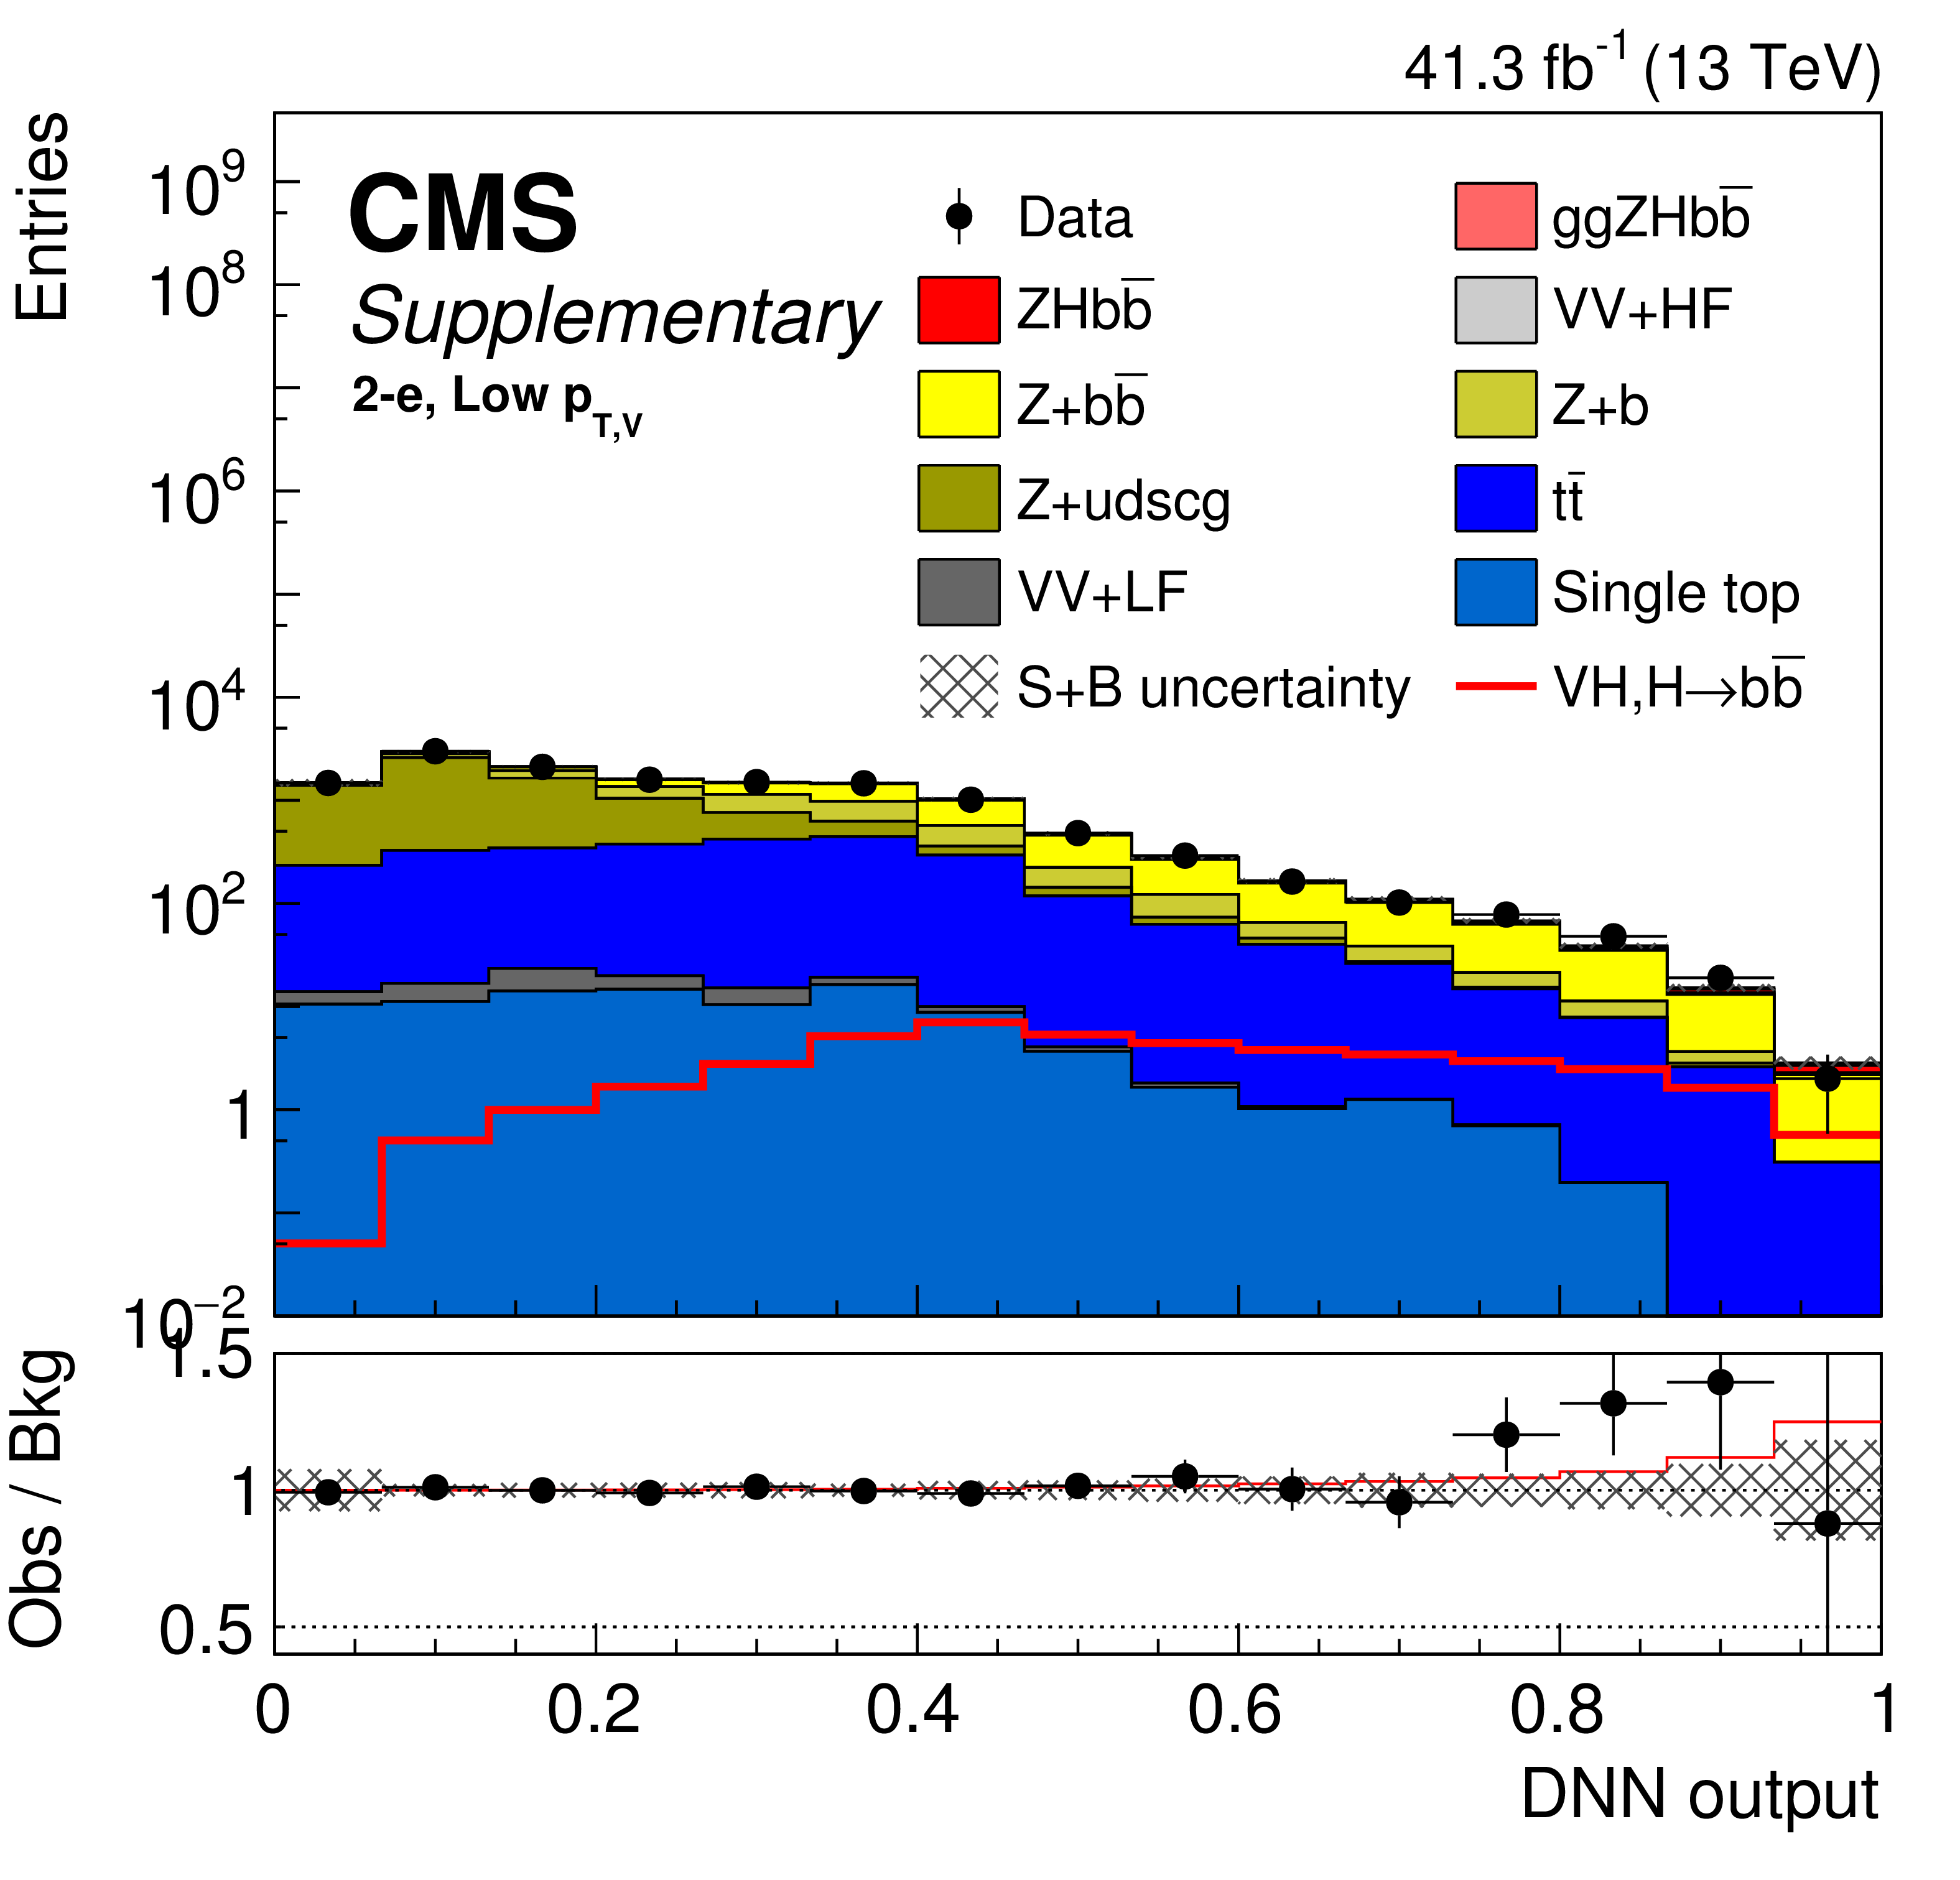
\includegraphics[width=0.285\linewidth]{images/SR_VHbb/CMS-HIG-18-016_Figure-aux_007-d}} \qquad
    \subfigure [] {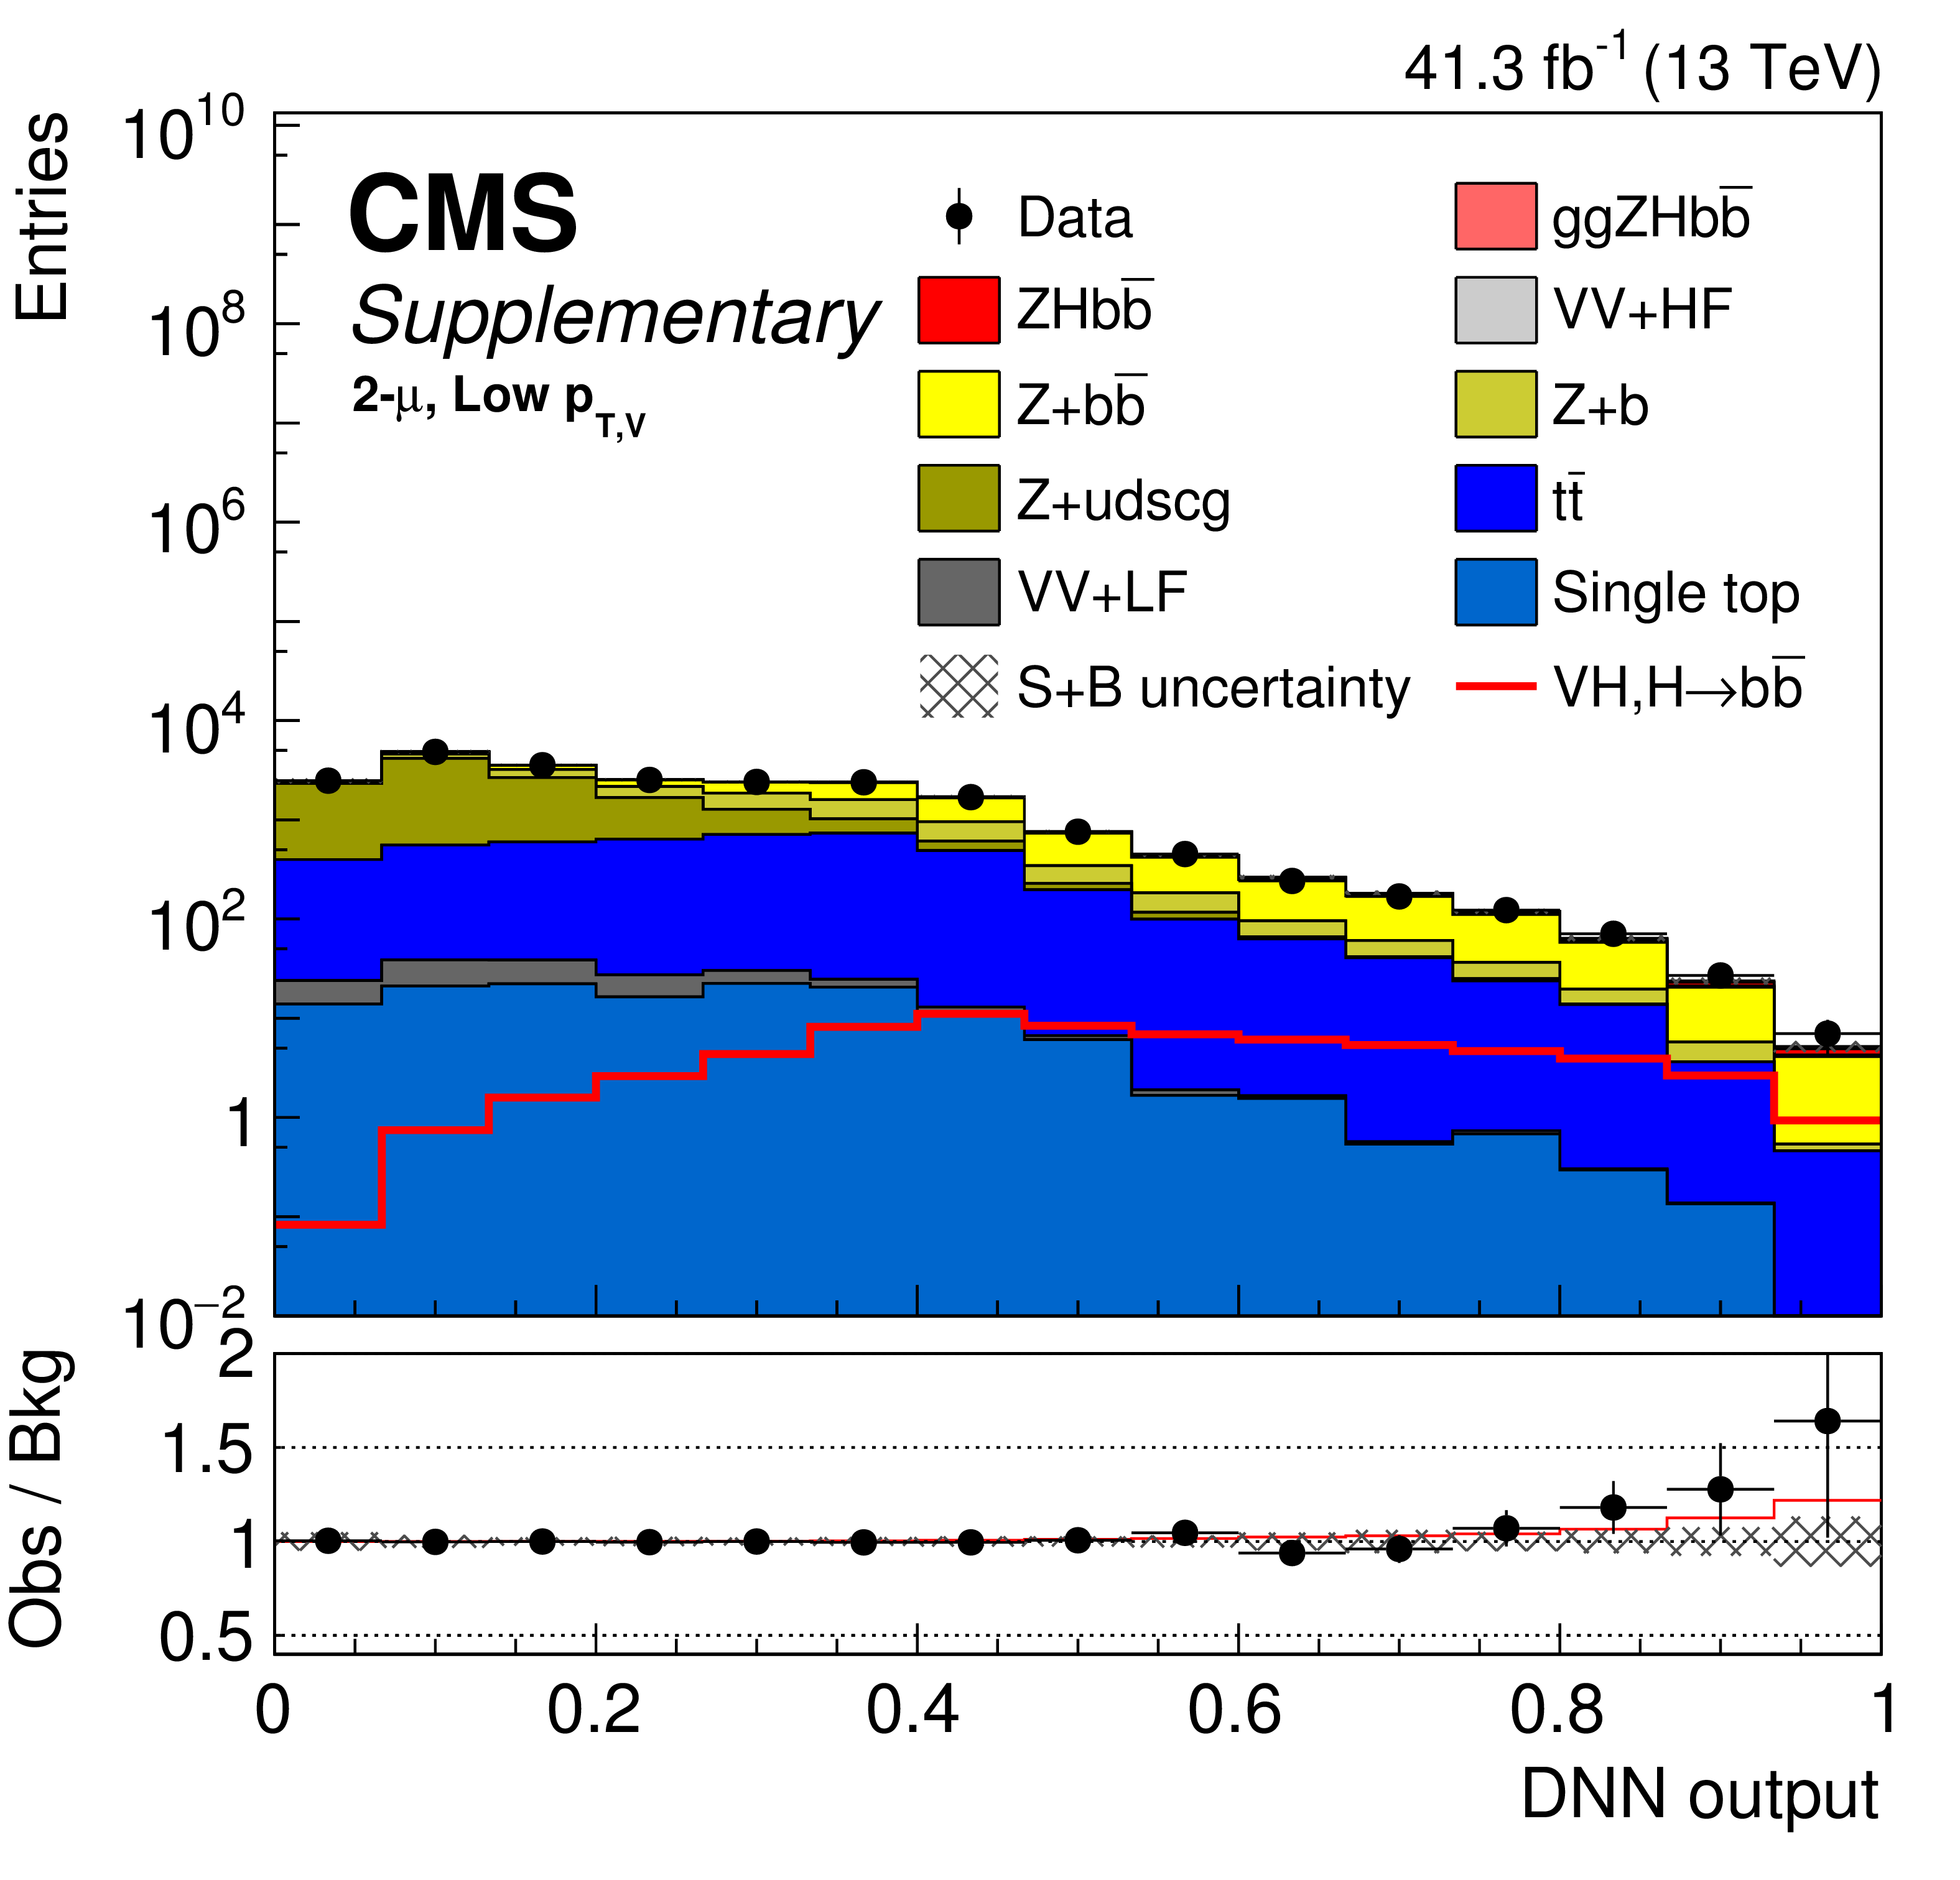
\includegraphics[width=0.285\linewidth]{images/SR_VHbb/CMS-HIG-18-016_Figure-aux_007-c}} \qquad
  }
  \mbox{
    \subfigure [] {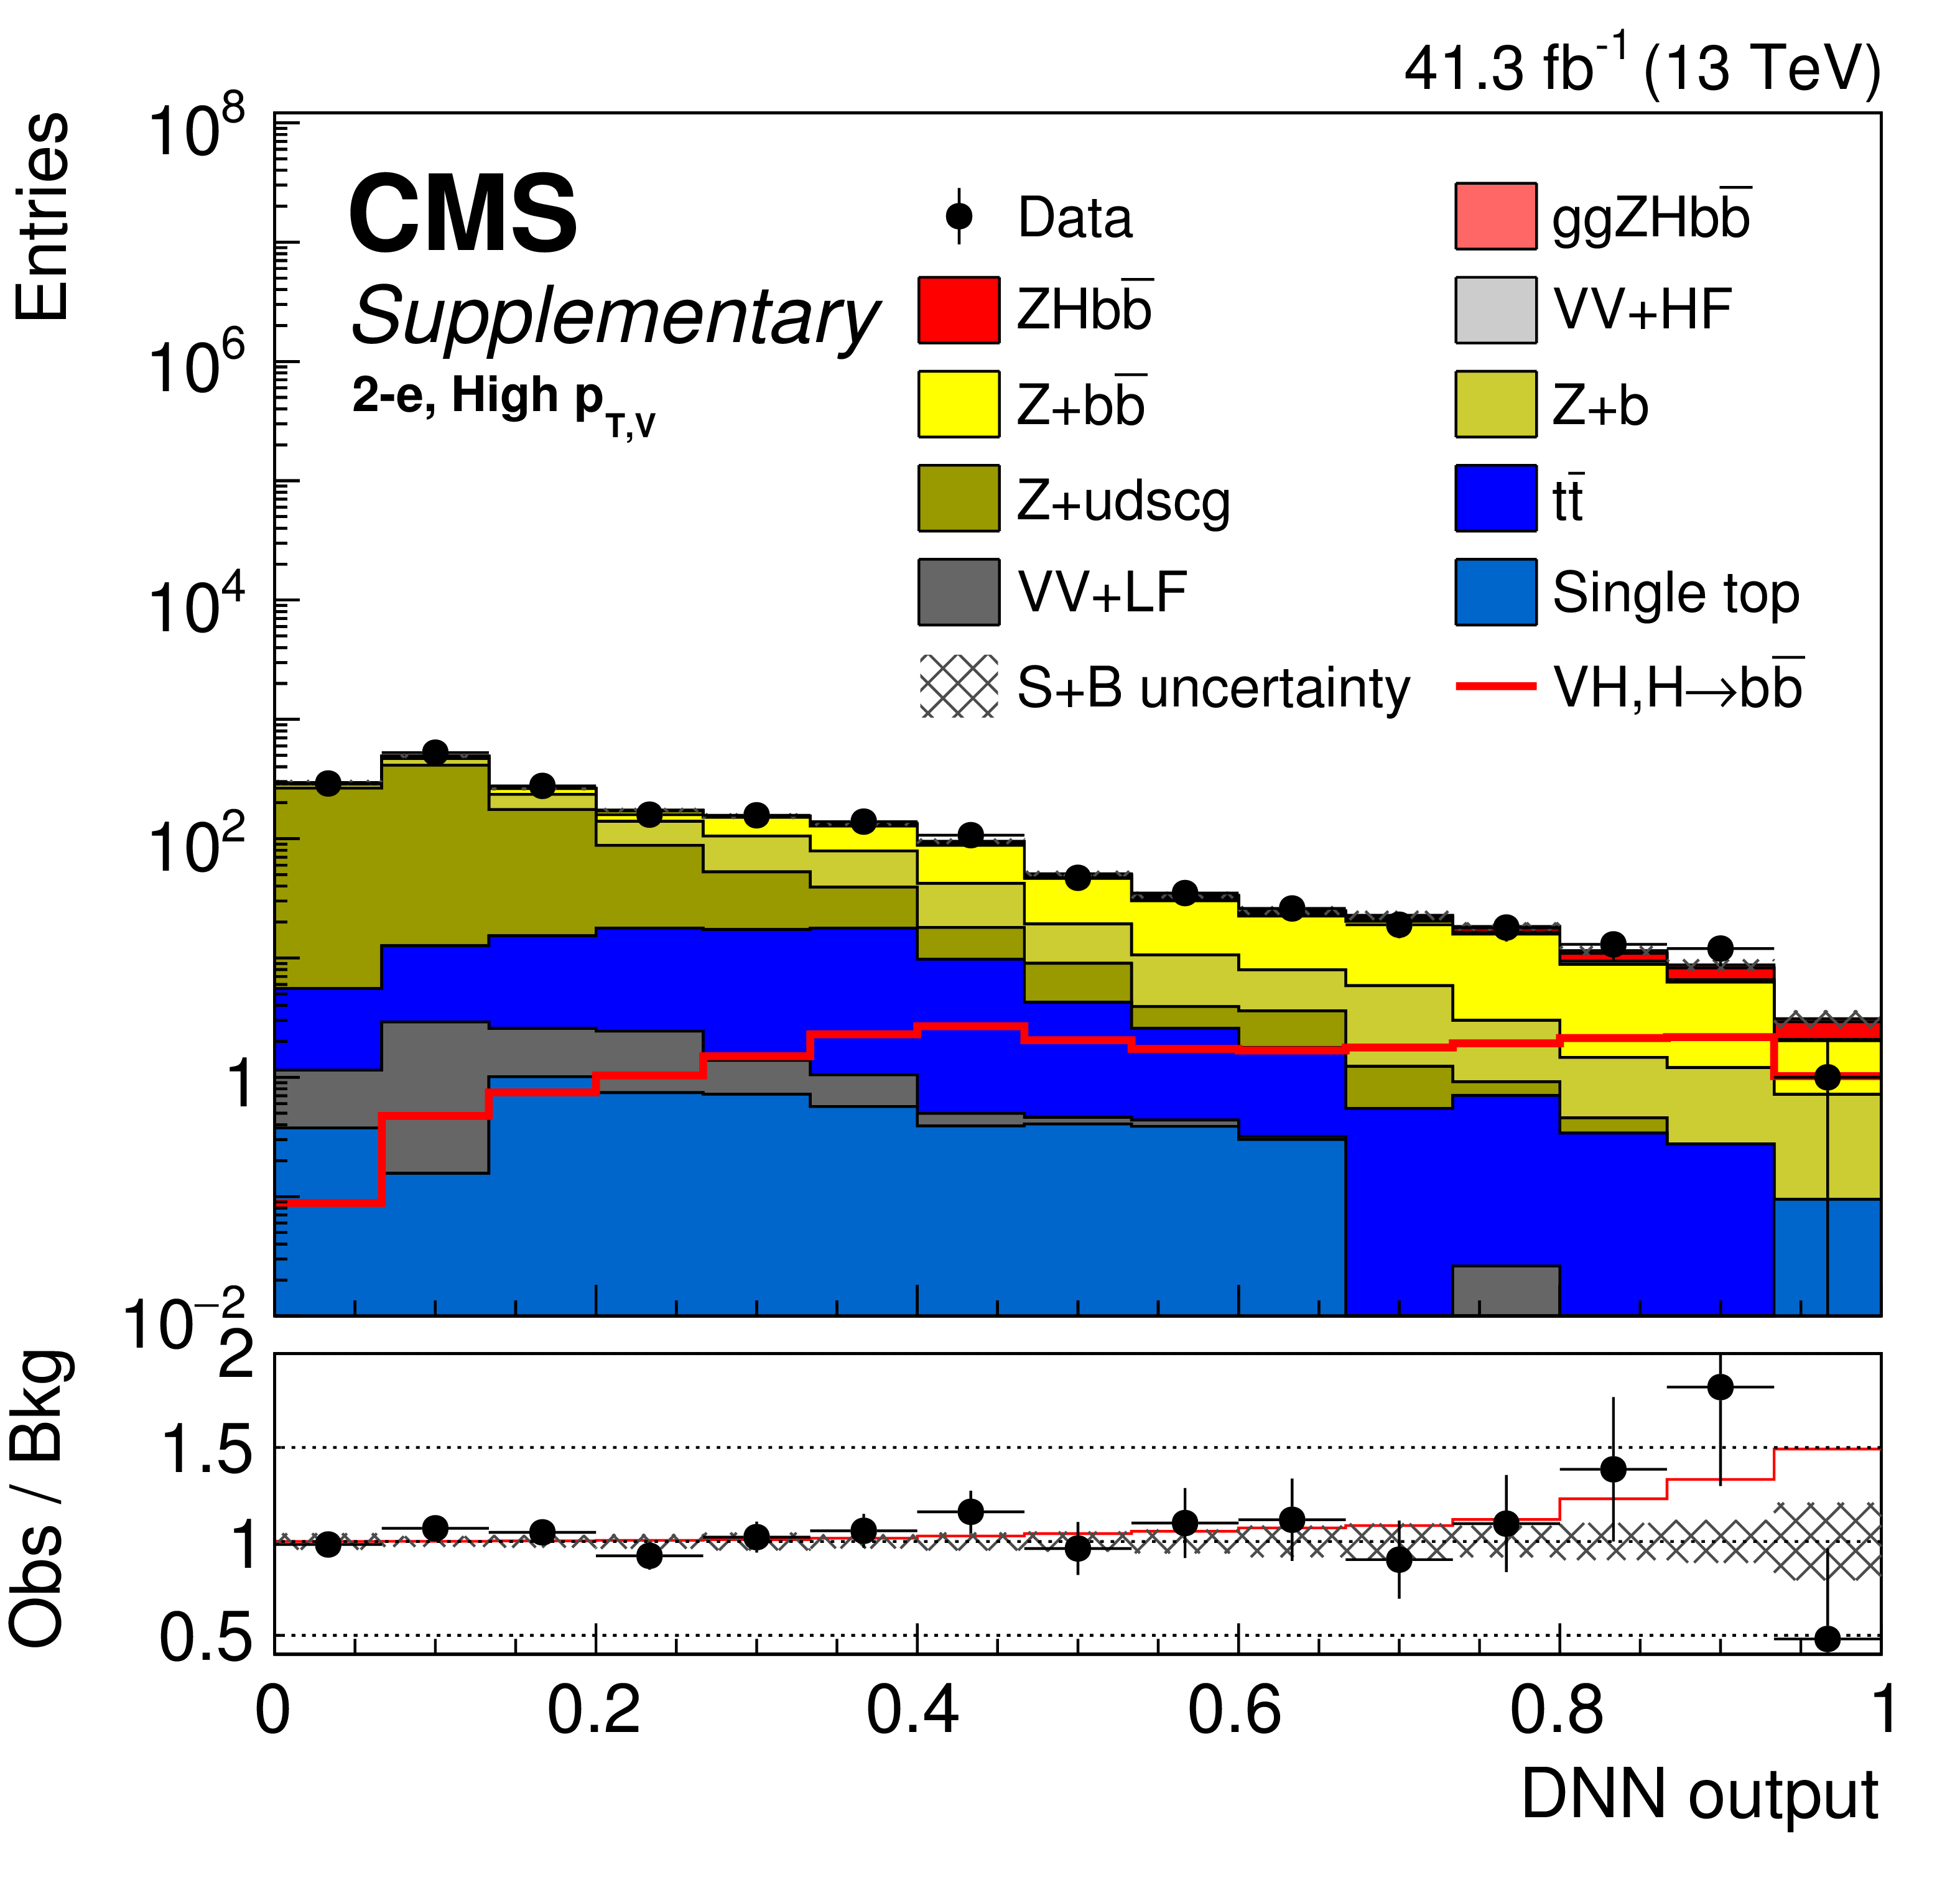
\includegraphics[width=0.285\linewidth]{images/SR_VHbb/CMS-HIG-18-016_Figure-aux_007-b}} \qquad
    \subfigure [] {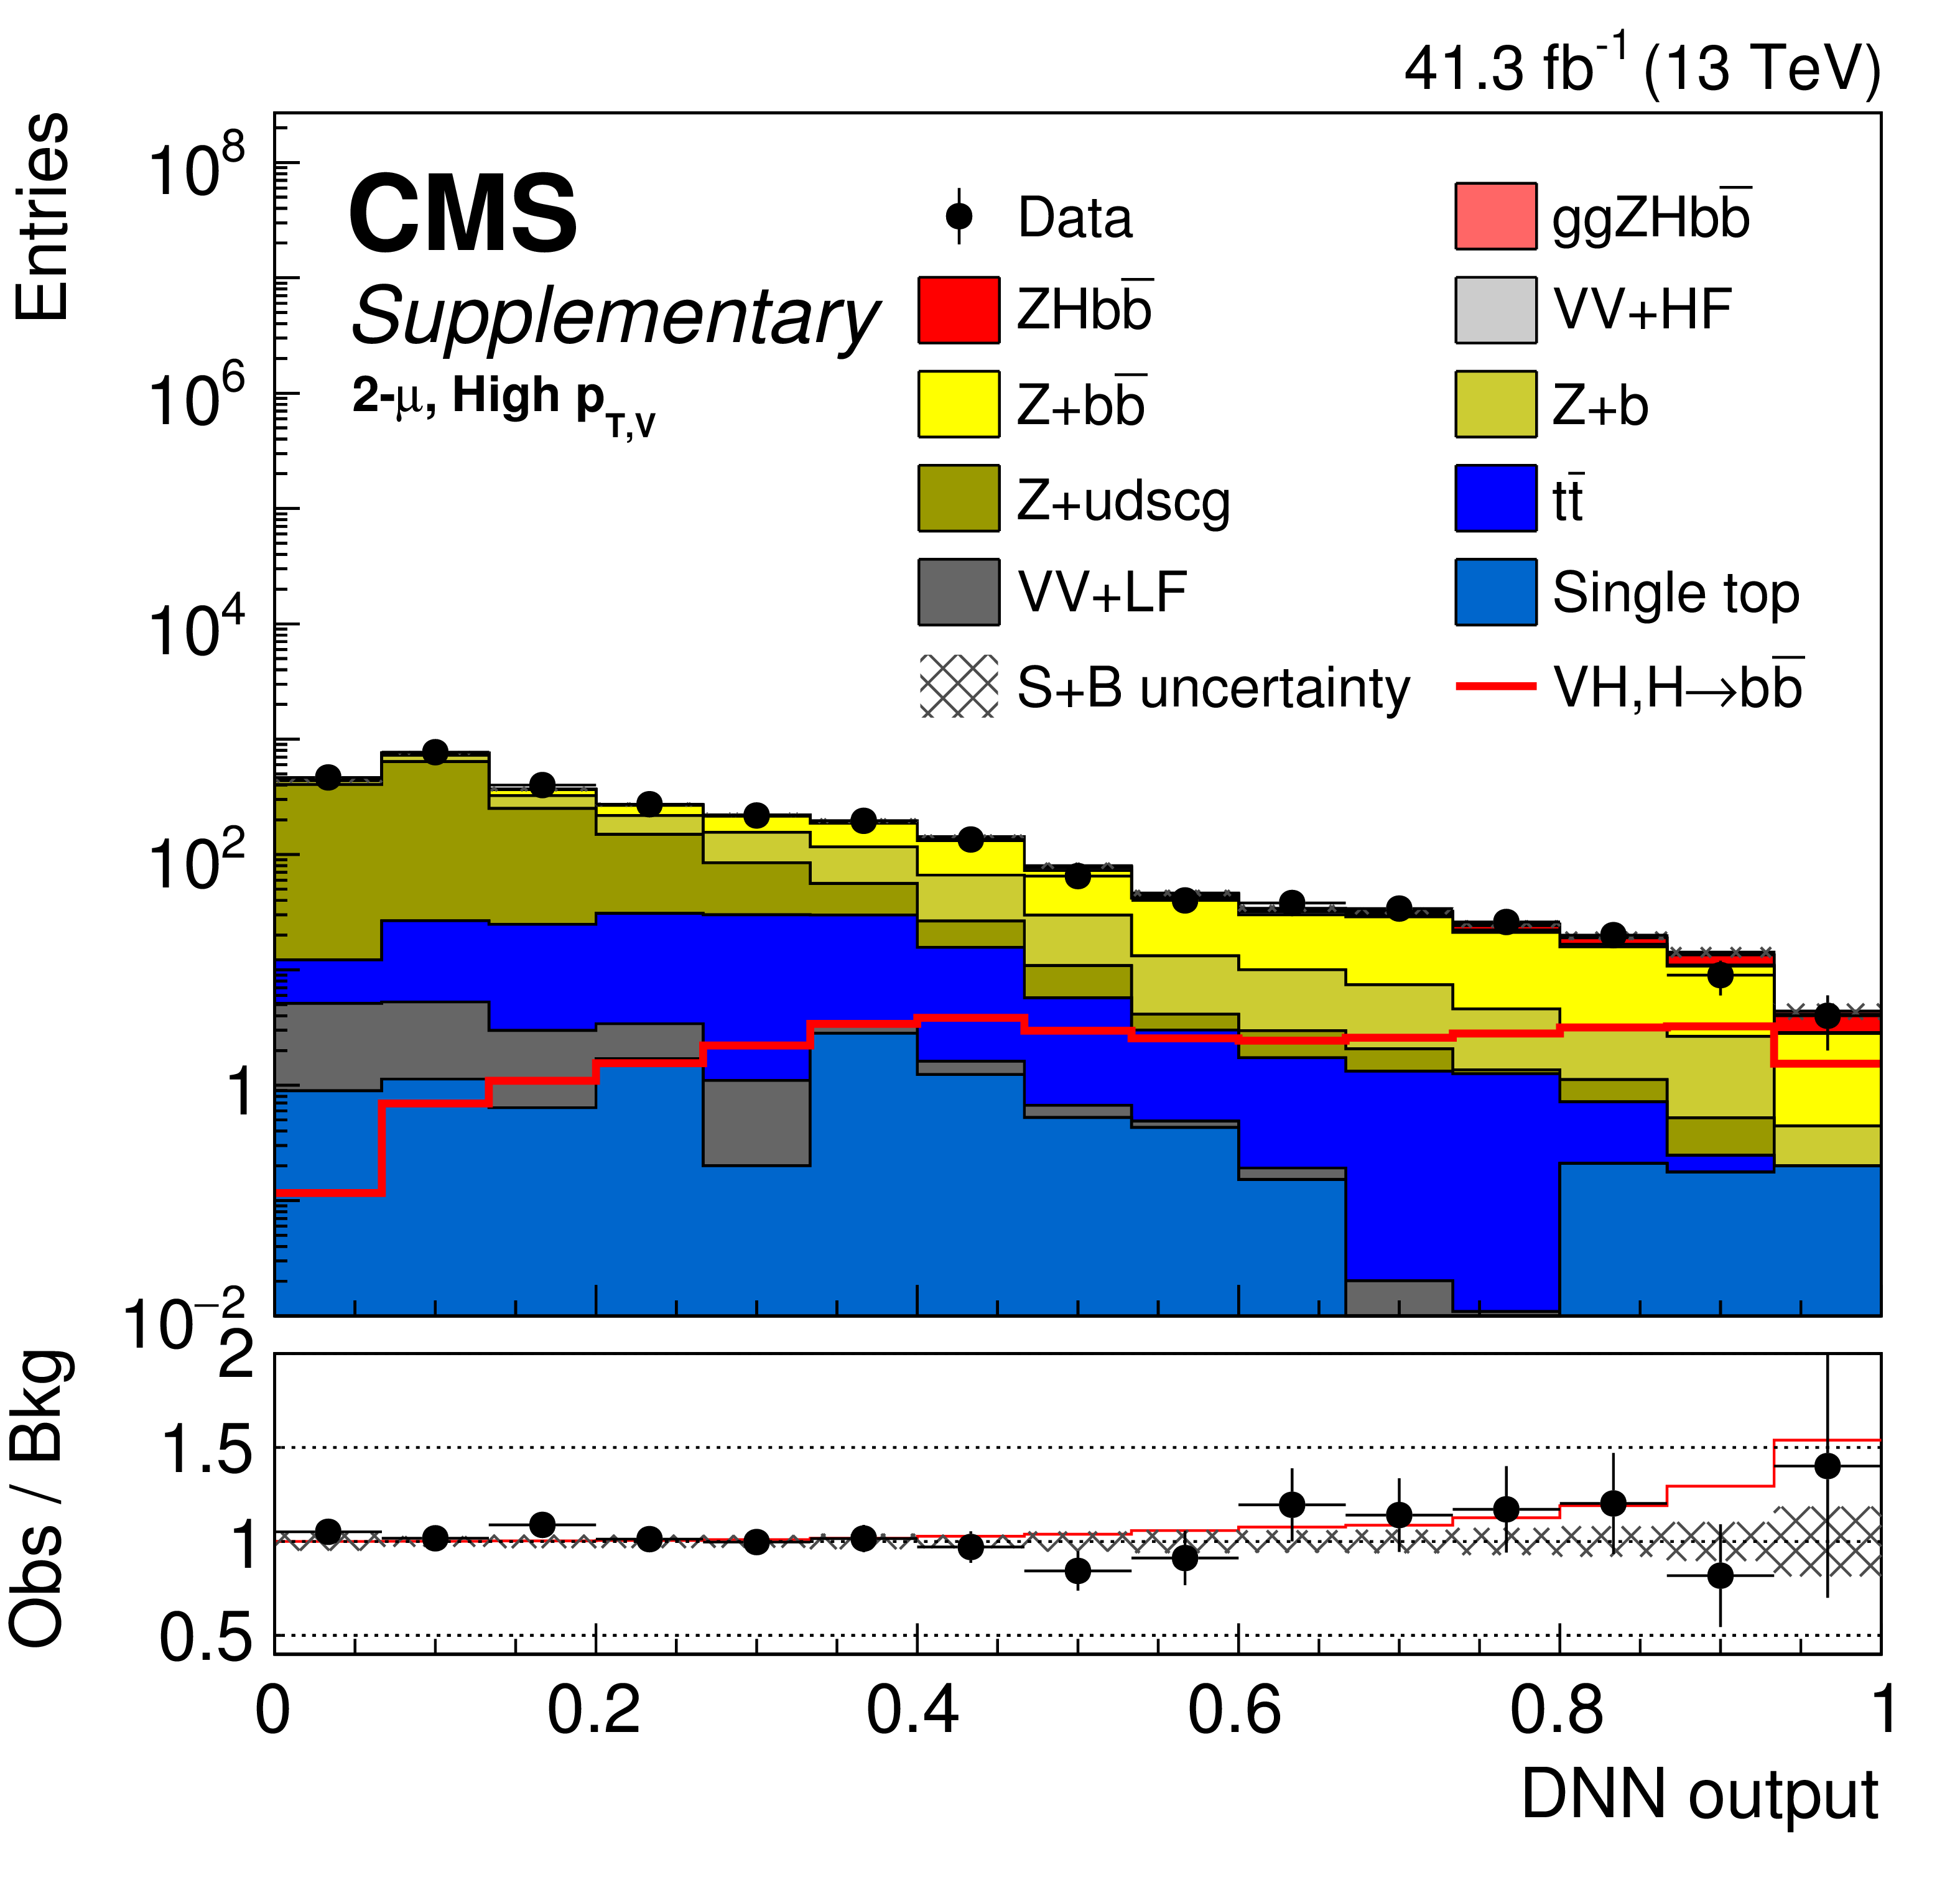
\includegraphics[width=0.285\linewidth]{images/SR_VHbb/CMS-HIG-18-016_Figure-aux_007-a}} \qquad
  }
  \mbox{
    \subfigure [] {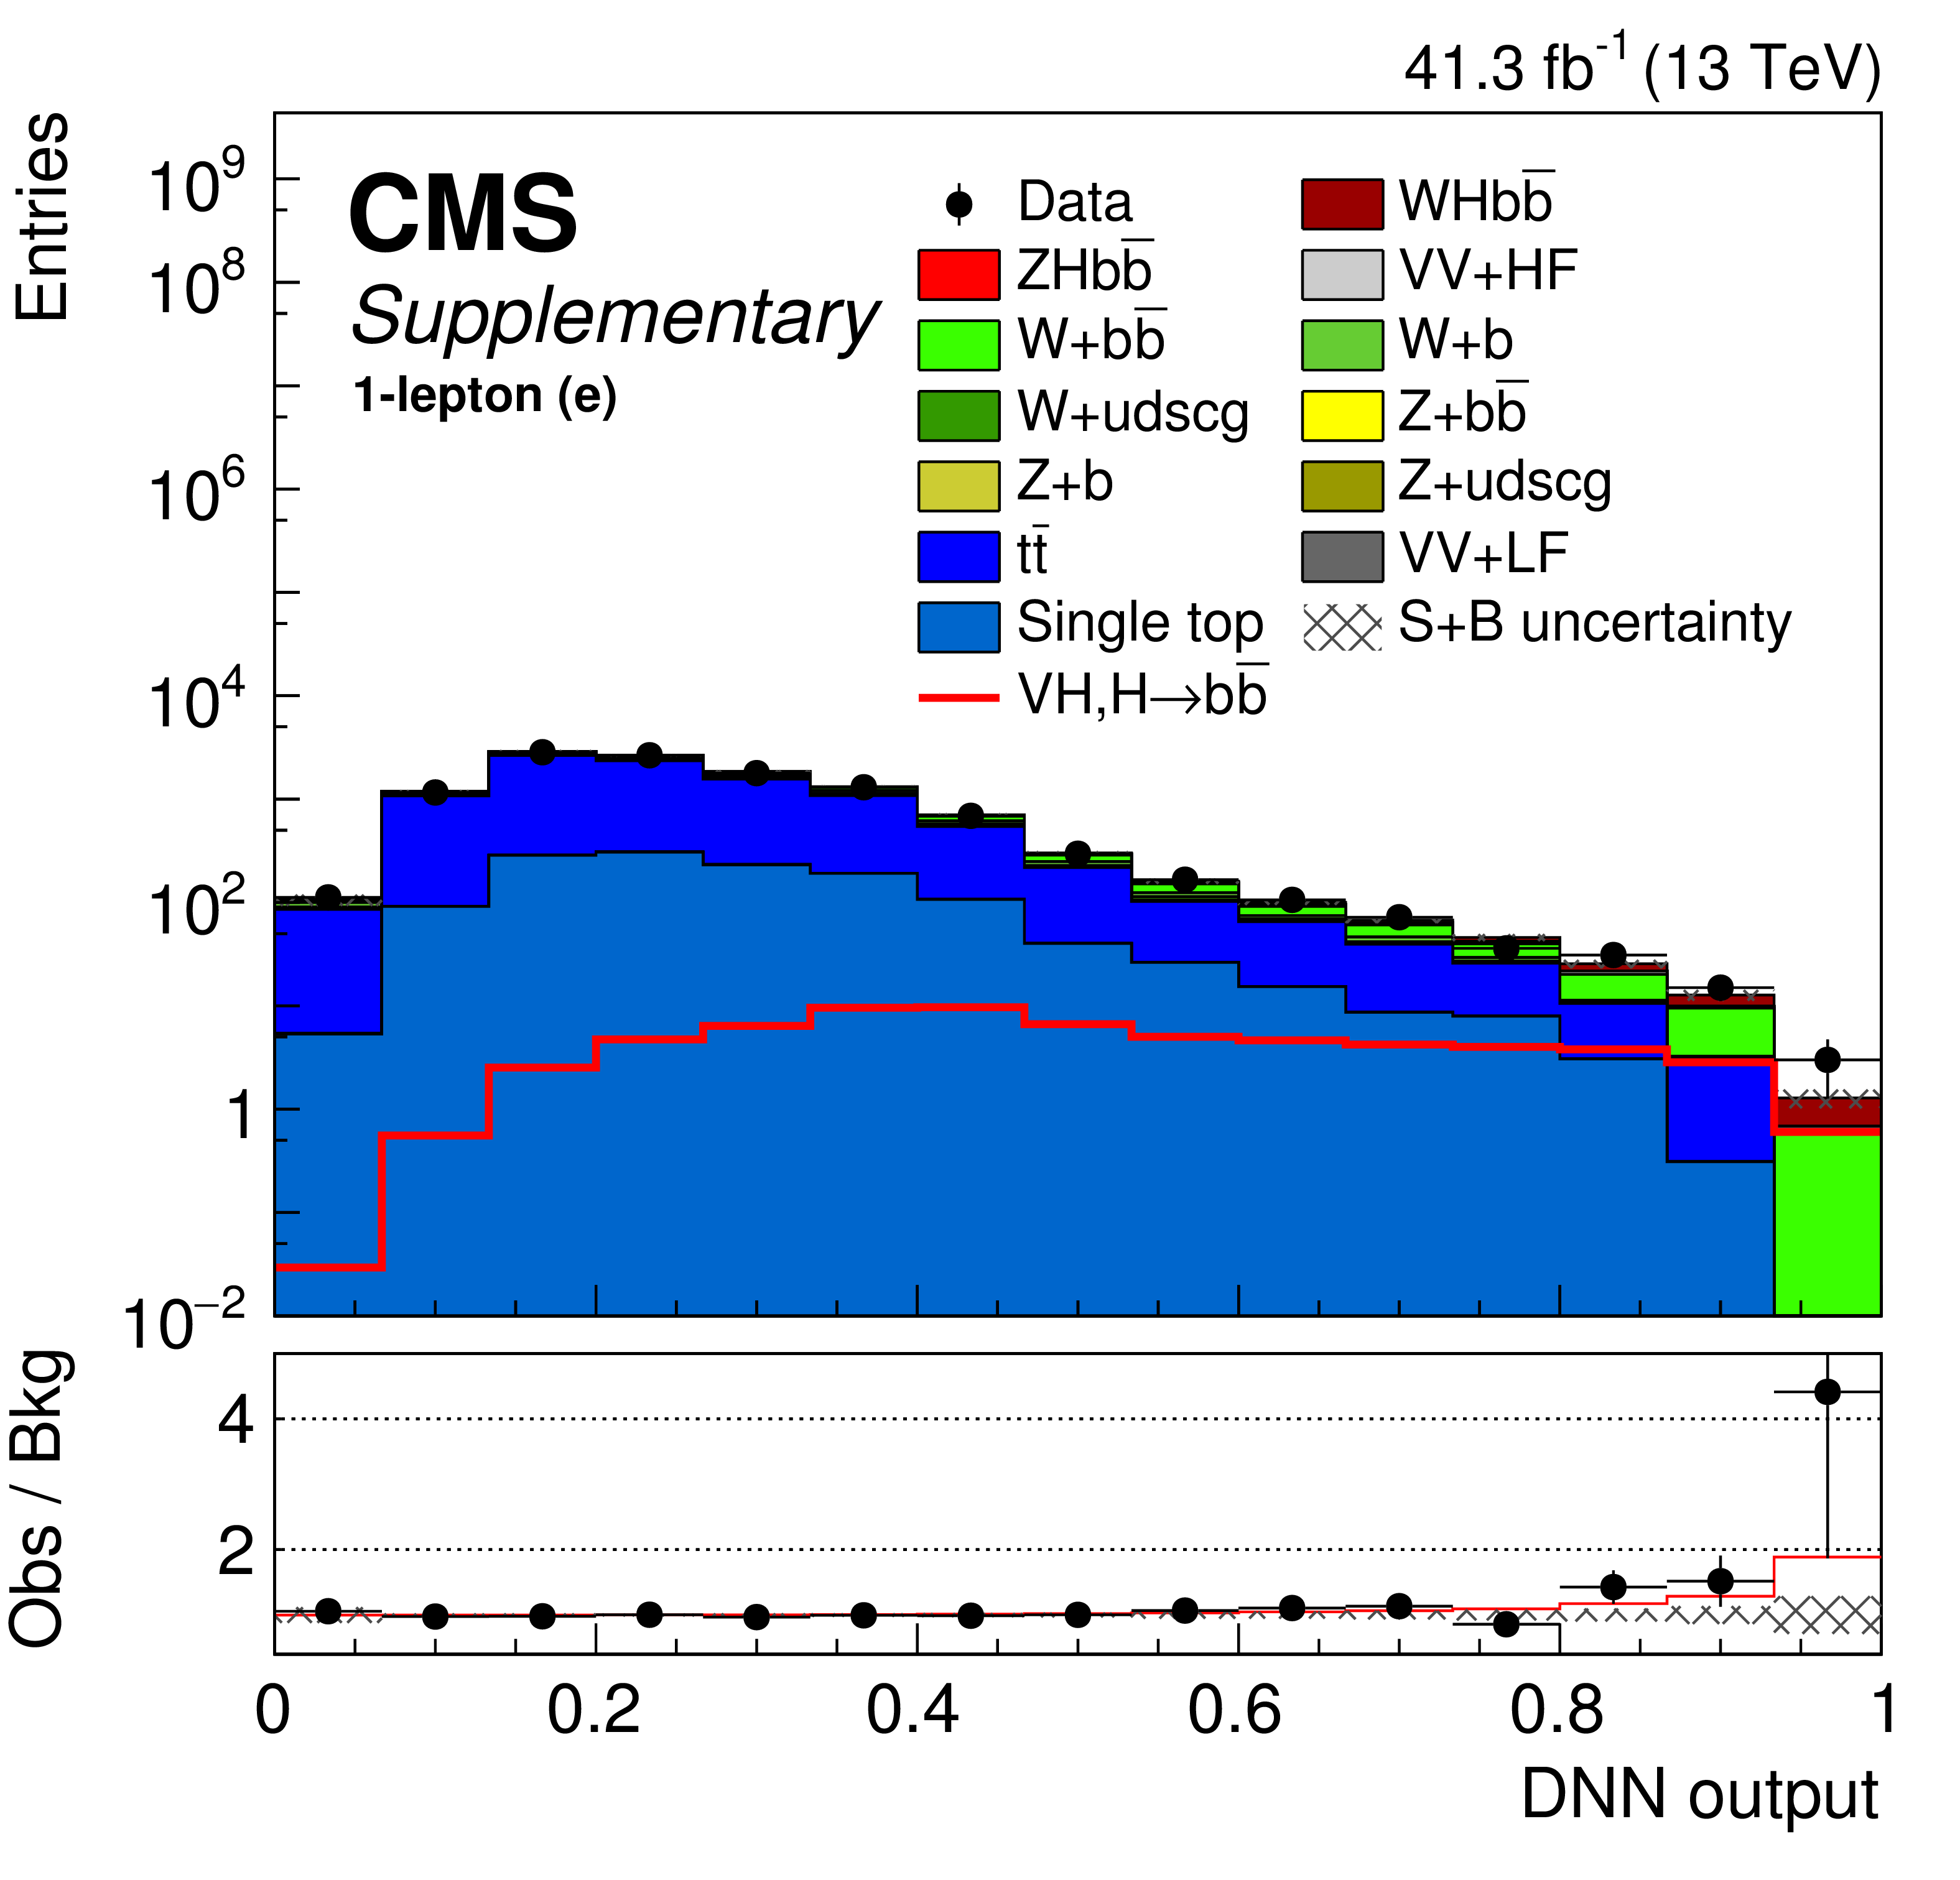
\includegraphics[width=0.285\linewidth]{images/SR_VHbb/CMS-HIG-18-016_Figure-aux_007-f}} \qquad
    \subfigure [] {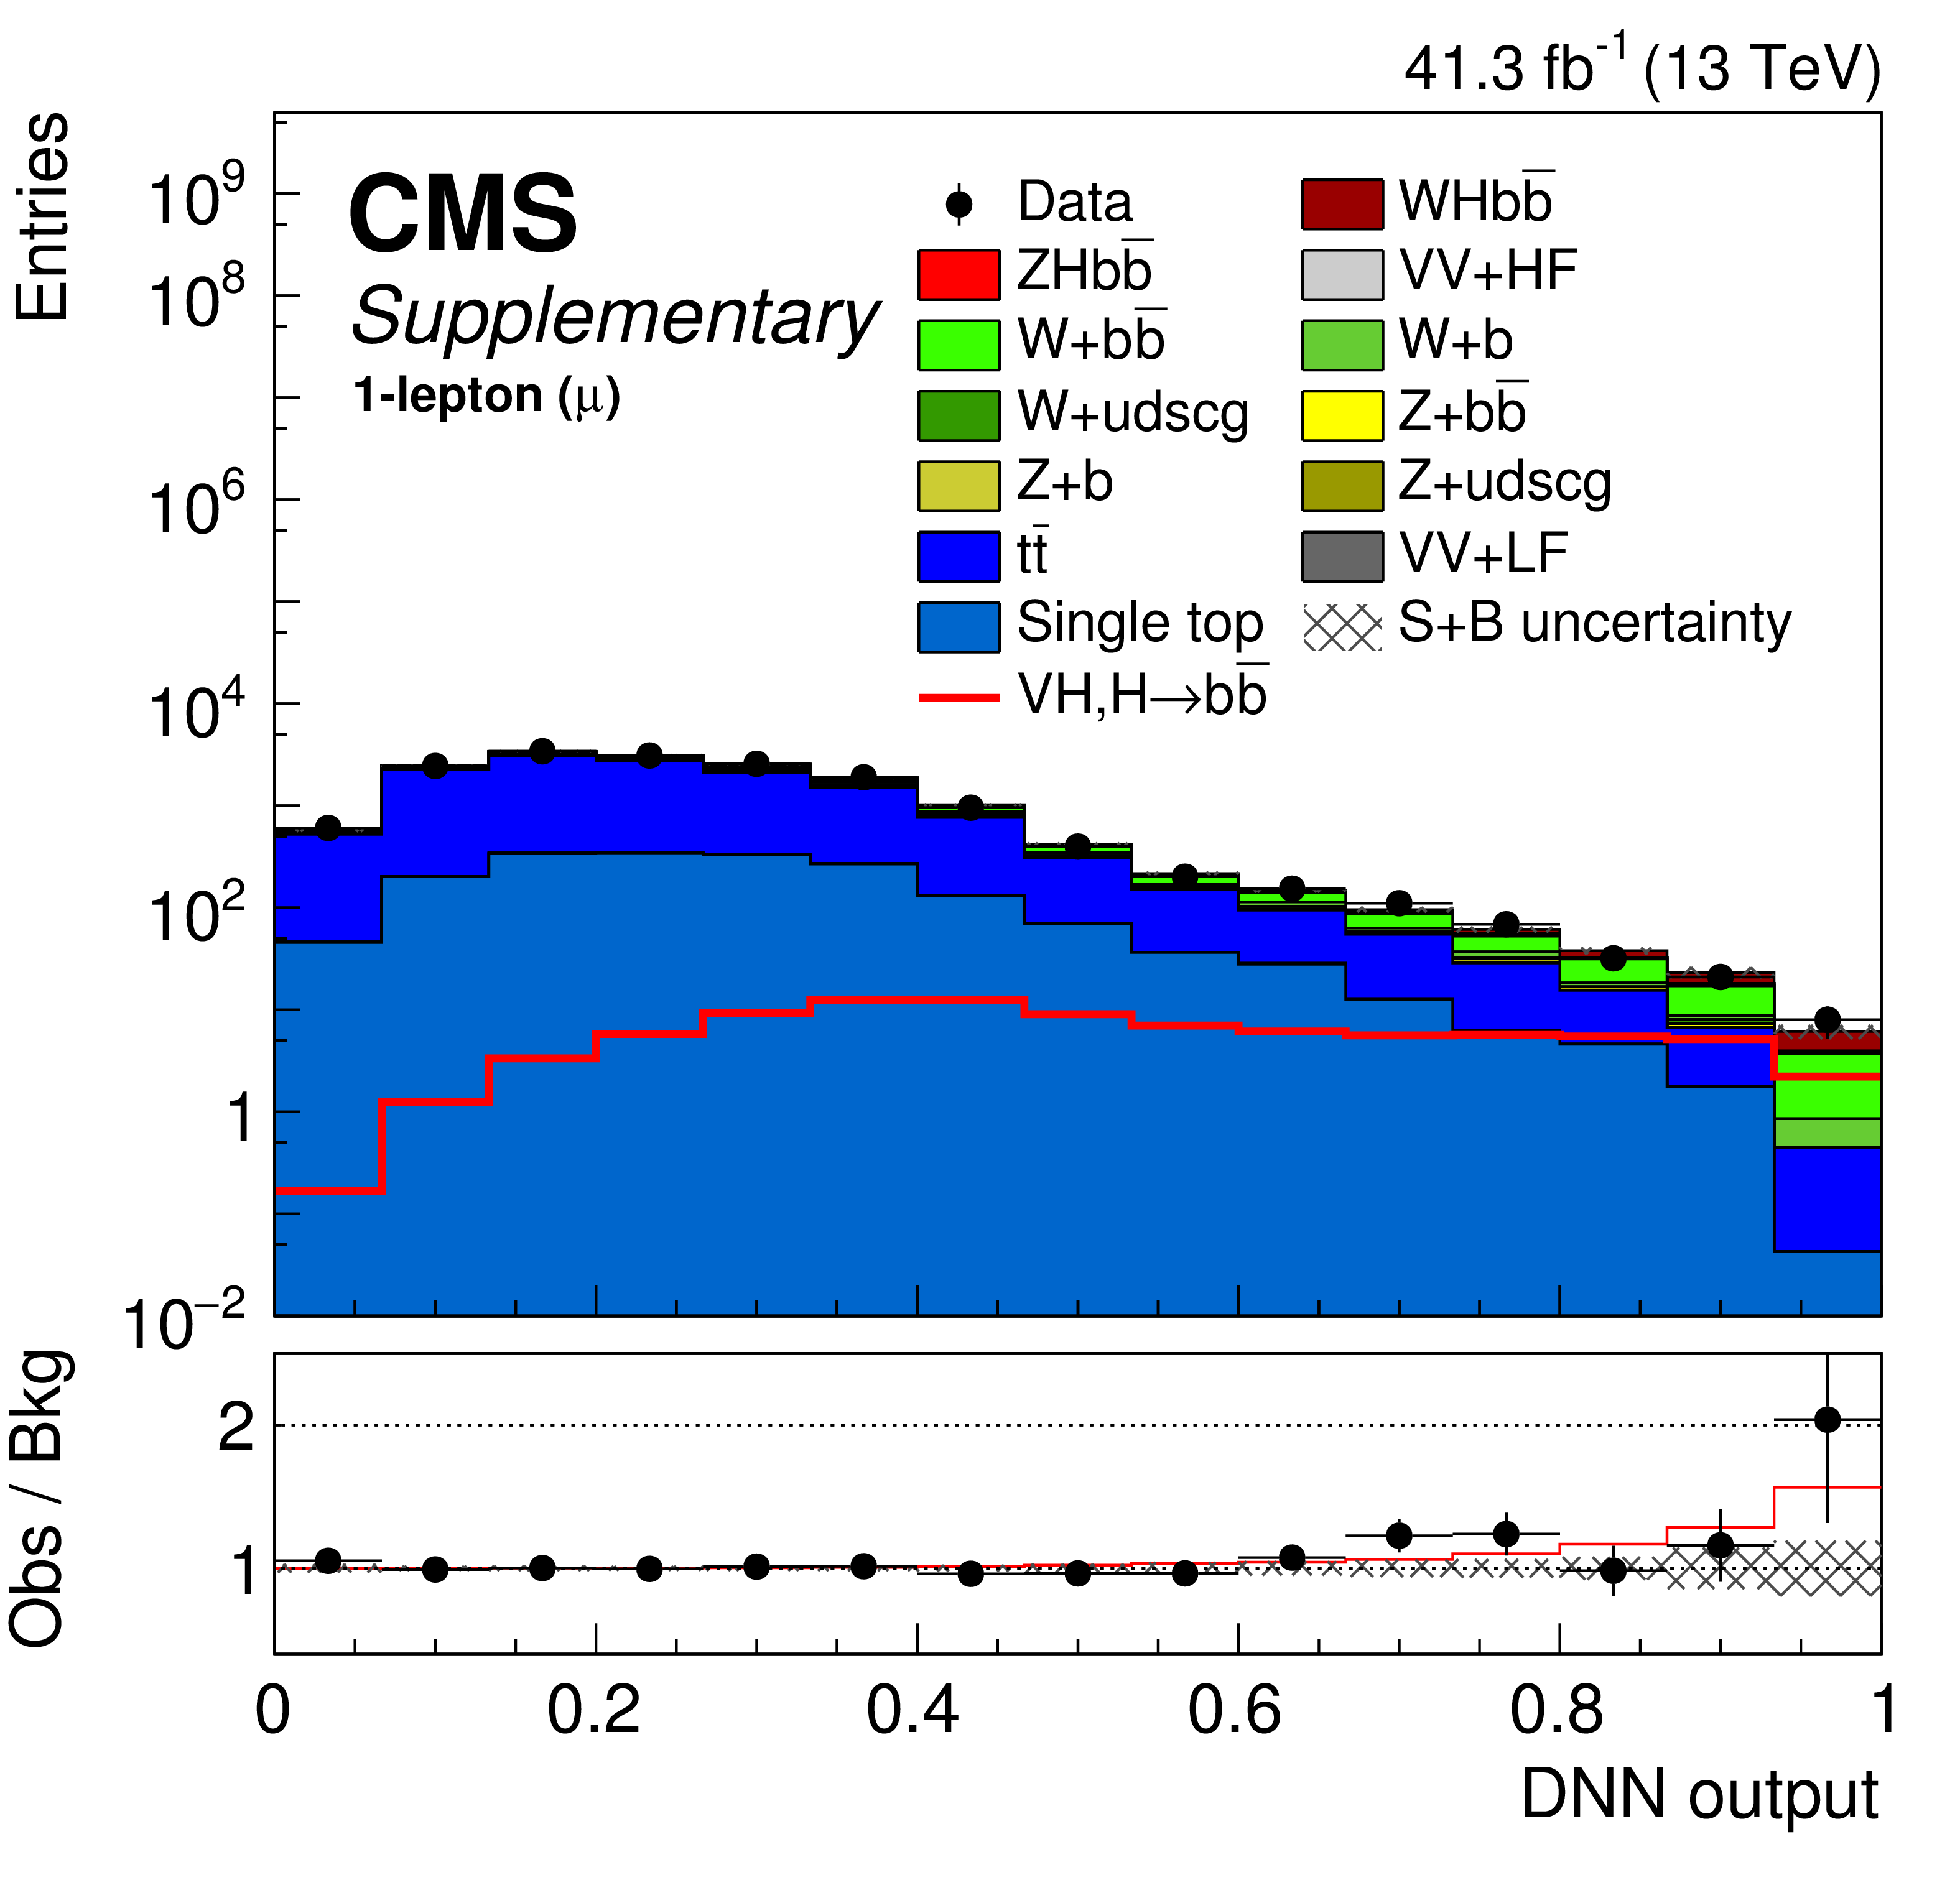
\includegraphics[width=0.285\linewidth]{images/SR_VHbb/CMS-HIG-18-016_Figure-aux_007-e}} \qquad
  }
  \mbox{
    \subfigure [] {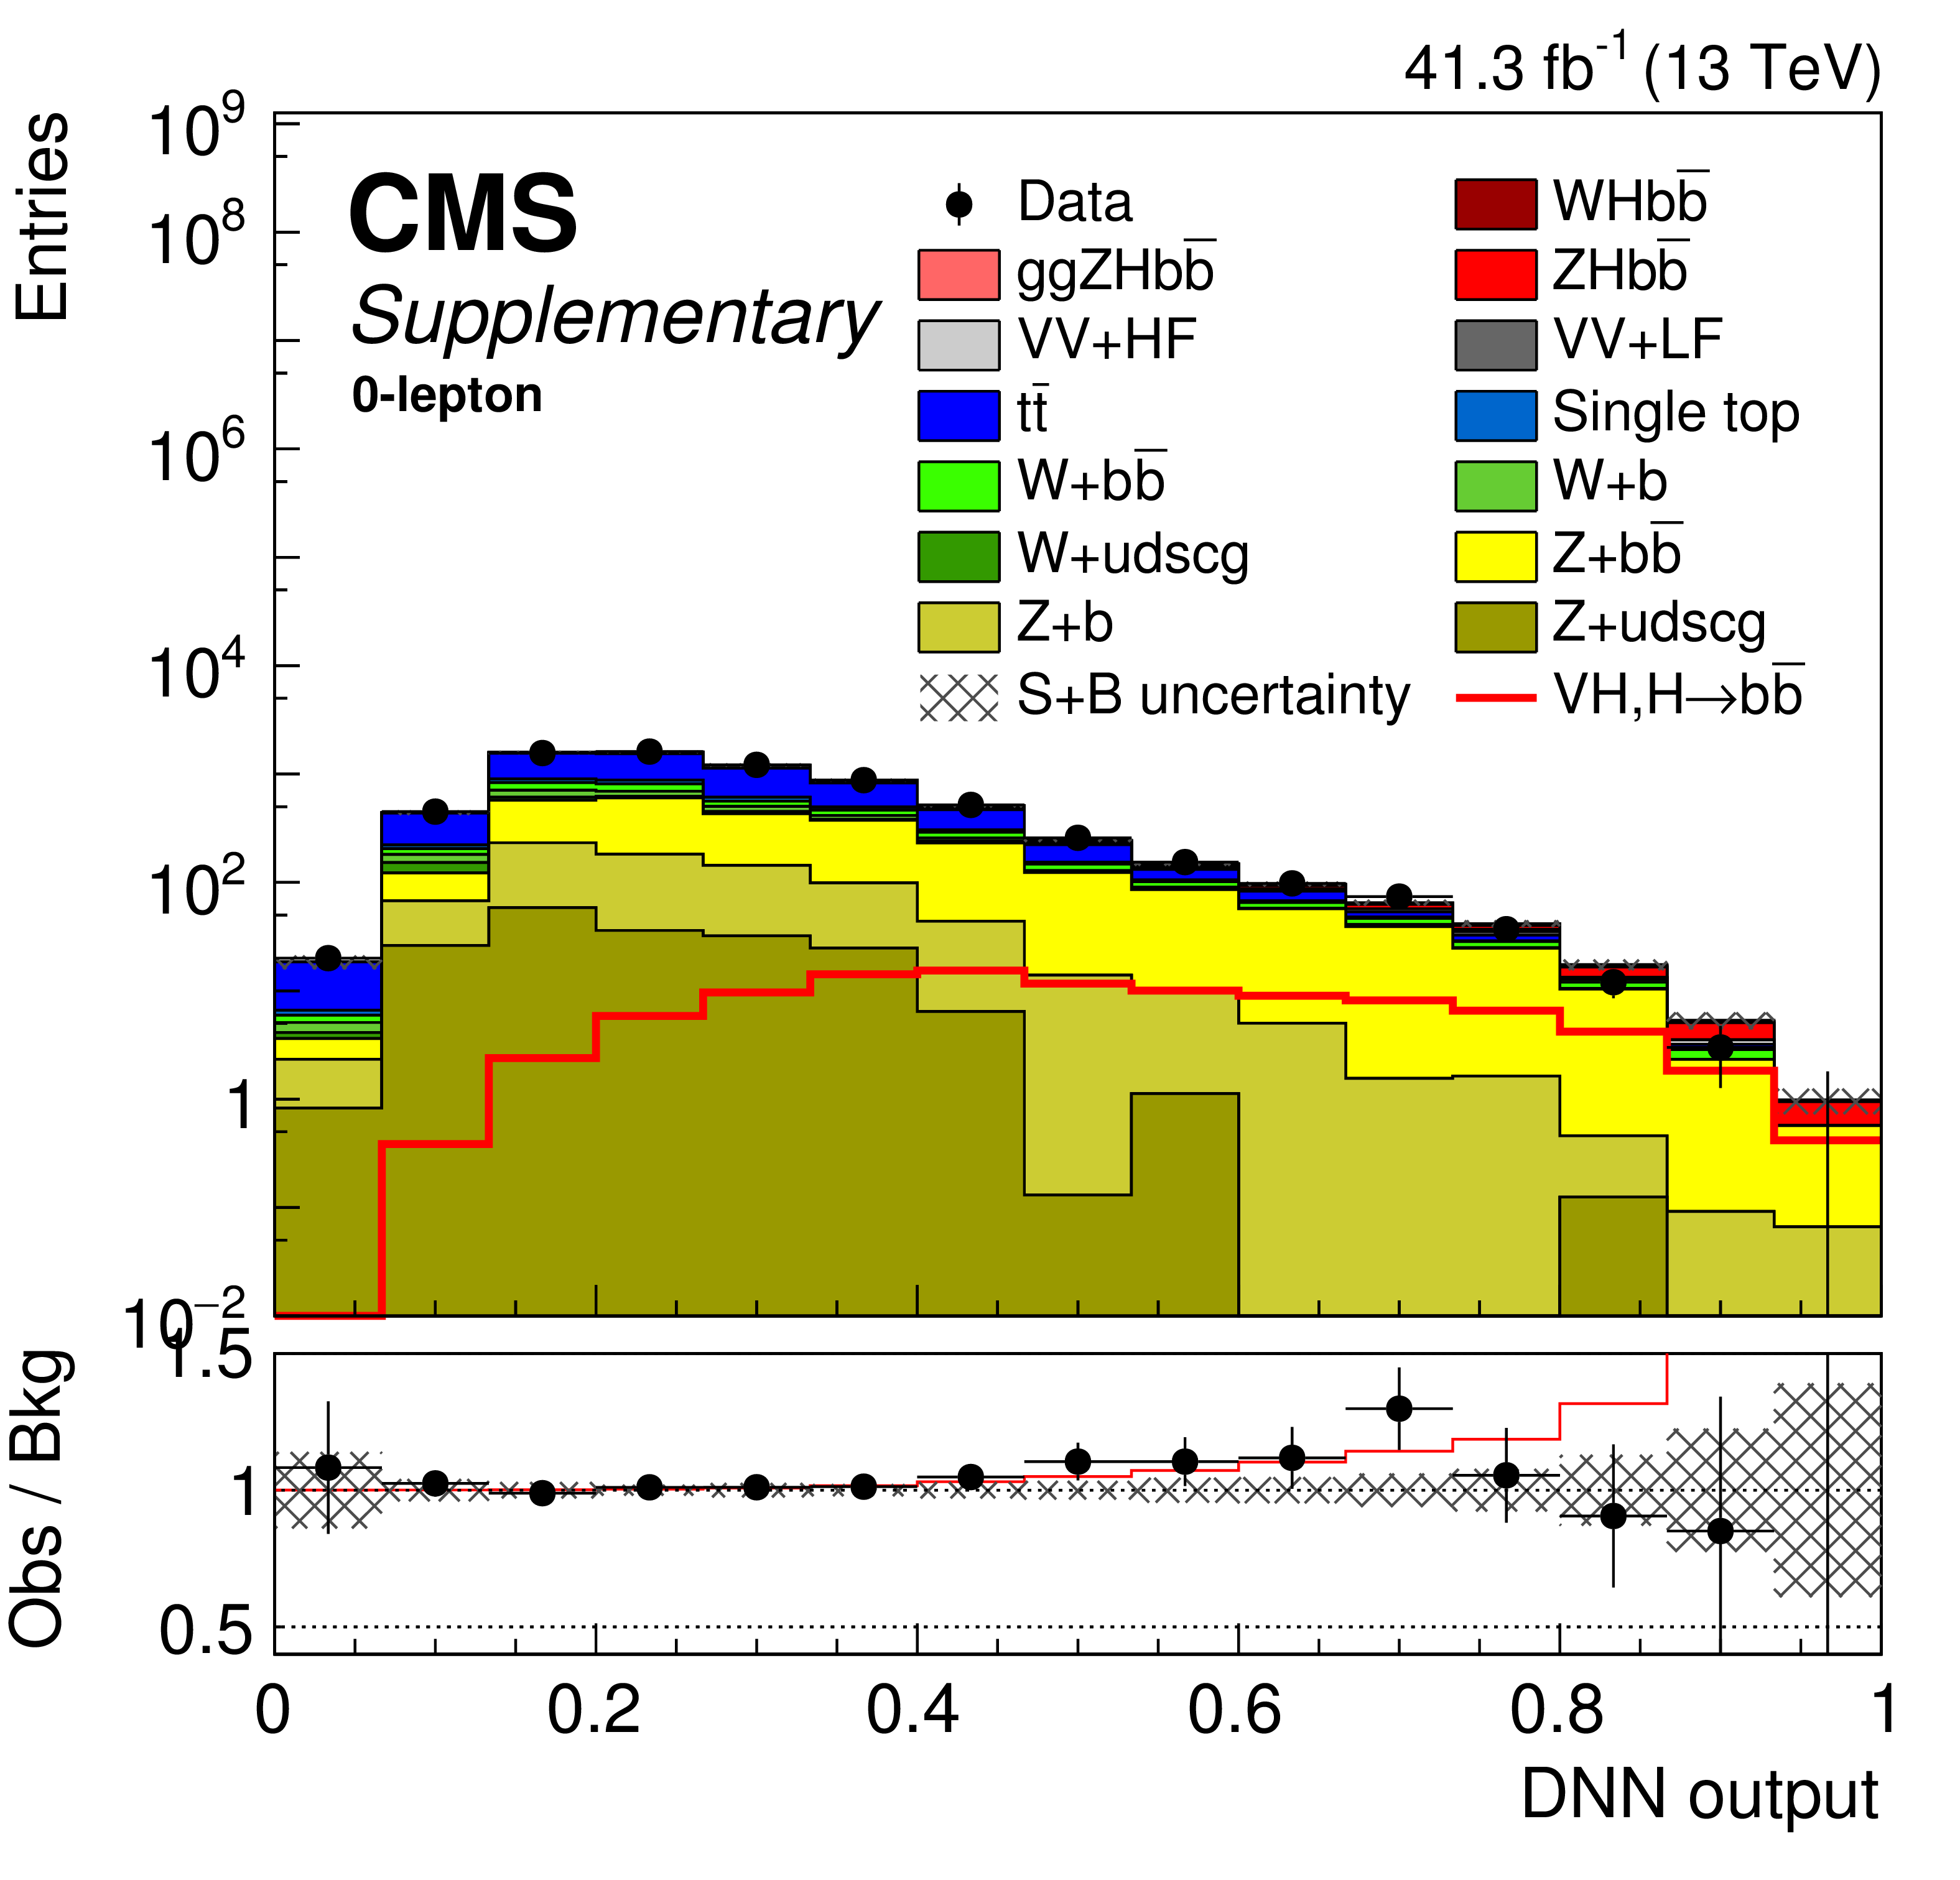
\includegraphics[width=0.285\linewidth]{images/SR_VHbb/CMS-HIG-18-016_Figure-aux_007-g}}
  }
  \caption[\VHbb\ Signal Region Distributions]{The post-fit \VHbb\ multivariate discriminant distributions of the A) low \pT(\bosV) \ZeeH; B) low \pT(\bosV) \ZmmH; C) high \pT(\bosV) \ZeeH; D) high \pT(\bosV) \ZmmH; E) \WenH; F) \WmnH; and G) \ZnnH\ channels.}
  \label{fig:SRVHbb}
\end{figure}

\begin{figure}[htbp]
  \centering
    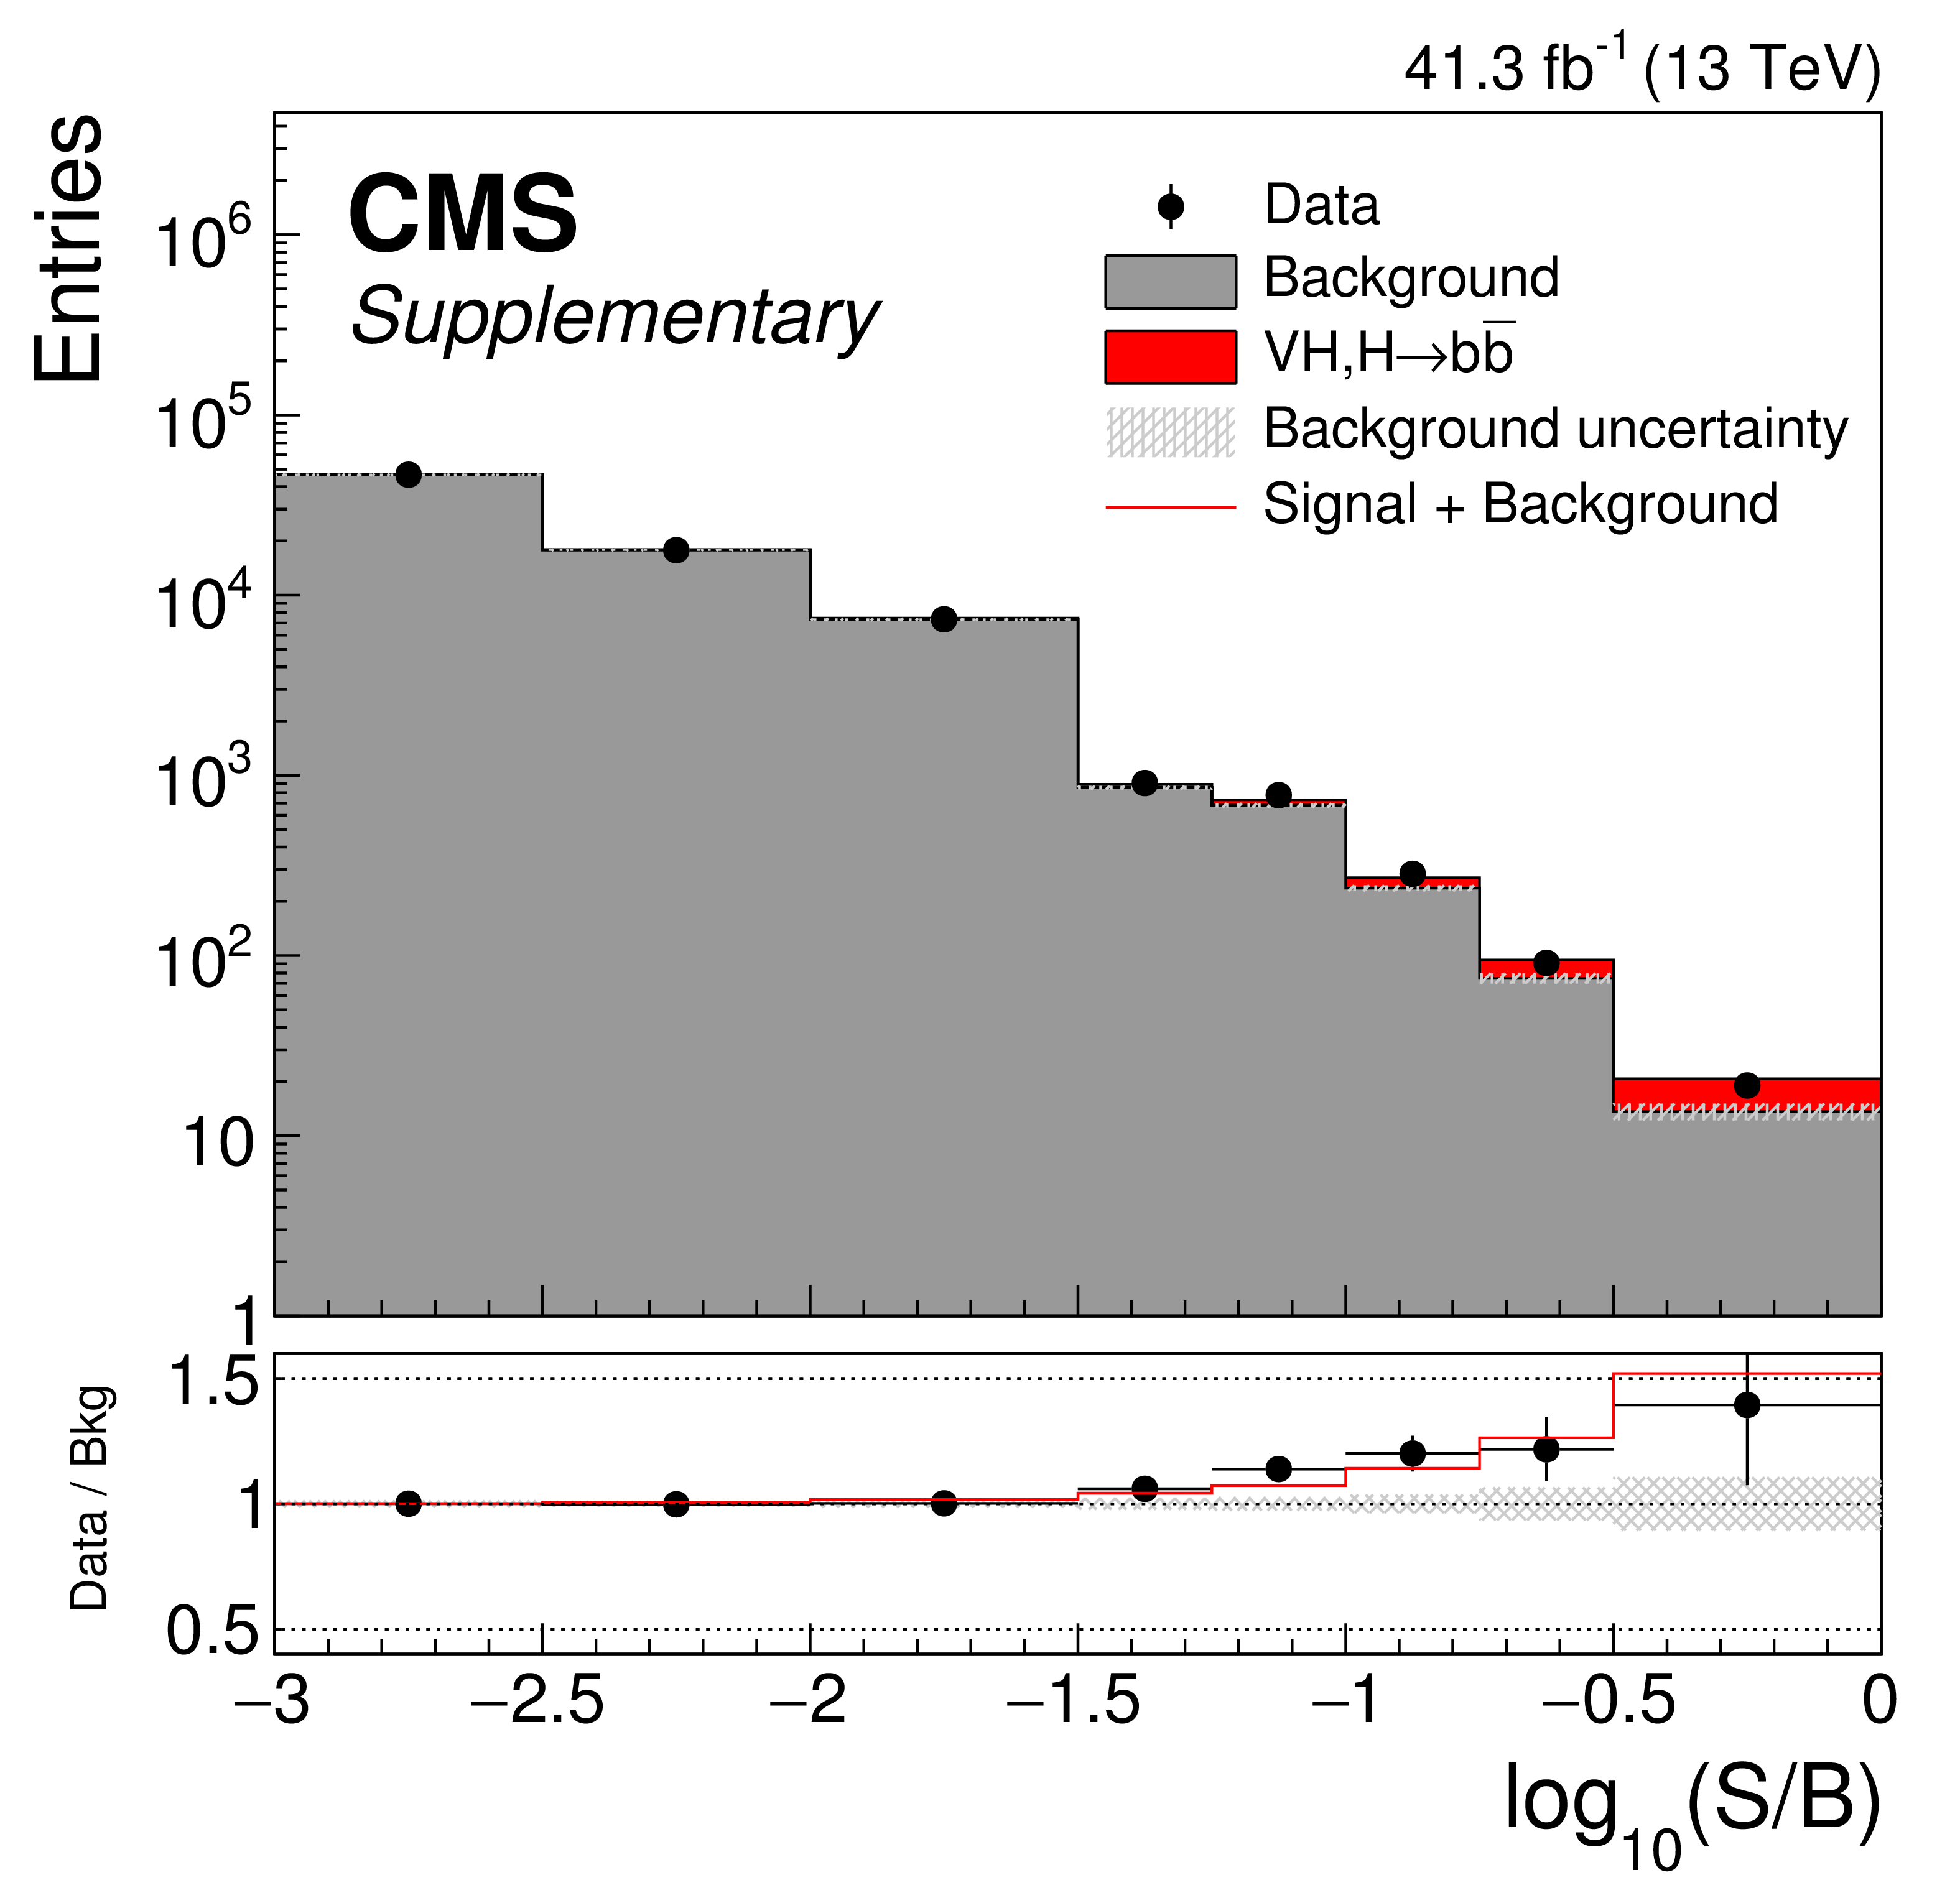
\includegraphics[width=3.5in]{images/CMS-HIG-18-016_Figure-aux_008-a}
    \caption[\VHbb\ Combined Signal Region Distribution]{The post-fit multivariate discriminant distributions of signal, background, and data event yields combined for all \VHbb\ channels and sorted into bins of similar signal-to-background ratio. The \VHbb\ signal contribution (red) has been stacked above the sum of all background yields (gray). The bottom panel shows the data to background ratio (black points) and the sum of signal and background contributions divided by the background yield (red line).}
    \label{fig:SBVHbb}
\end{figure}

\begin{figure}[htbp]
  \centering
    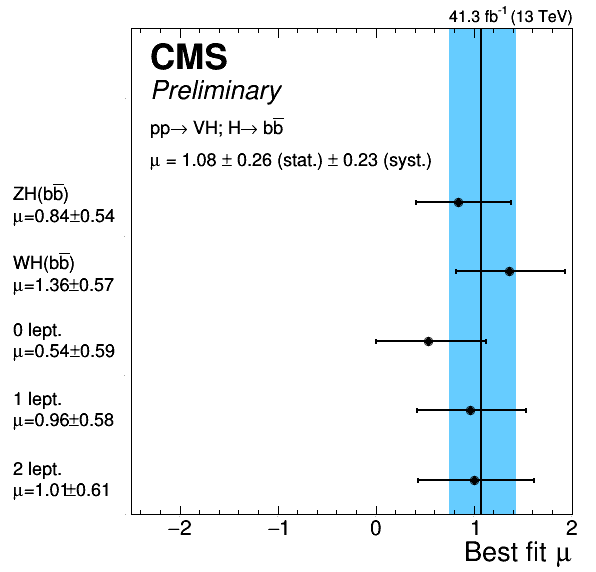
\includegraphics[width=3.5in]{images/MuVHbb}
    \caption[\VHbb\ Analysis Signal Strengths]{The best fit signal strengths and their uncertainties for each of the channels of the \VHbb\ analysis.}
    \label{fig:MuVHbb}
\end{figure}

\begin{table}[htbp]
  \caption[\VHbb\ Main Uncertainty Sources]{The contributions of the main uncertainty sources in the measurement of the \VHbb\ signal strength. Due to correlations between the nuisance parameters of different sources in the maximum likelihood fit, the sum in quadrature of each source is not necessarily the total uncertainty of each major component.}
  \label{tbl:UncVHbb}
  \begin{tabularx}{6.5in}{Xcc}
    \hline
    Uncertainty Source                        & \multicolumn{2}{c}{$\Delta\mu$} \\
    \hline
    Theory                                    & $+0.11$        & $-0.09$        \\
    - Signal theory                           & $+0.07$        & $-0.04$        \\
    - Background theory                       & $+0.08$        & $-0.08$        \\
    Size of simulated samples                 & $+0.12$        & $-0.12$        \\
    Experimental                              & $+0.16$        & $-0.15$        \\
    - Luminosity                              & $+0.03$        & $-0.03$        \\
    - Lepton efficiency                       & $+0.02$        & $-0.01$        \\
    - Jet energy scale and resolution         & $+0.05$        & $-0.05$        \\
    - \qrkb-Tagging efficiency                & $+0.09$        & $-0.08$        \\
    - Other experimental uncertainties        & $+0.10$        & $-0.09$        \\
    Statistical                               & $+0.26$        & $-0.26$        \\
    - Background control region normalization & $+0.12$        & $-0.12$        \\
    Total                                     & $+0.35$        & $-0.33$        \\
    \hline
  \end{tabularx}
\end{table}

\section{Combinations with Past CMS Results}

A combination of the 2017 \VHbb\ analysis results with those of the 2016 \VHbb\ analysis published in Ref. \cite{CMSVHbbEvidence} increases the expected and observed significance to $4.16\sigma$ and $4.36\sigma$, respectively, with a best fit signal strength of $\mu = 1.06_{-0.26}^{+0.25}$. A further combination of these analyses with the Run 1 analysis published in Ref. \cite{CMSVHbbRun1} further increases the expected and observed significance to $4.88\sigma$ and $4.82\sigma$, respectively, with a best fit signal strength of $\mu = 1.01_{-0.23}^{+0.22}$. The results of this combination fall short of establishing an observation of the \VHbb\ decay.

A global fit is performed that combines all available CMS analyses of different \Htobb\ production processes, including this analysis of \VHbb, gluon fusion\cite{ggHbb}, vector boson fusion\cite{VBF}, and \qrkt\qrktbar\ associated production\cite{CMSttH1,CMSttH2,CMSttH3}. Because the results of these analyses span multiple datasets collected at 7, 8, and 13 \TeV\ and different detector operating conditions, most systematic uncertainty sources are treated as uncorrelated. For analyses using the same collision energies, the jet energy scale uncertainties are treated as correlated between those processes. The theoretical uncertainties are correlated between all processes and datasets. This grand combination achieves an expected and observed significance of $5.5\sigma$ and $5.6\sigma$, respectively. The best fit signal strength is $\mu = 1.04 \pm 0.20$, and the signal strengths of the different \Htobb\ production modes are shown in Figure \ref{fig:MuHbb}. This marks the first observation of the \Htobb\ decay at the CMS experiment and the measured signal strength indicates agreement with the Standard Model expectation.

\begin{figure}[htbp]
  \centering
    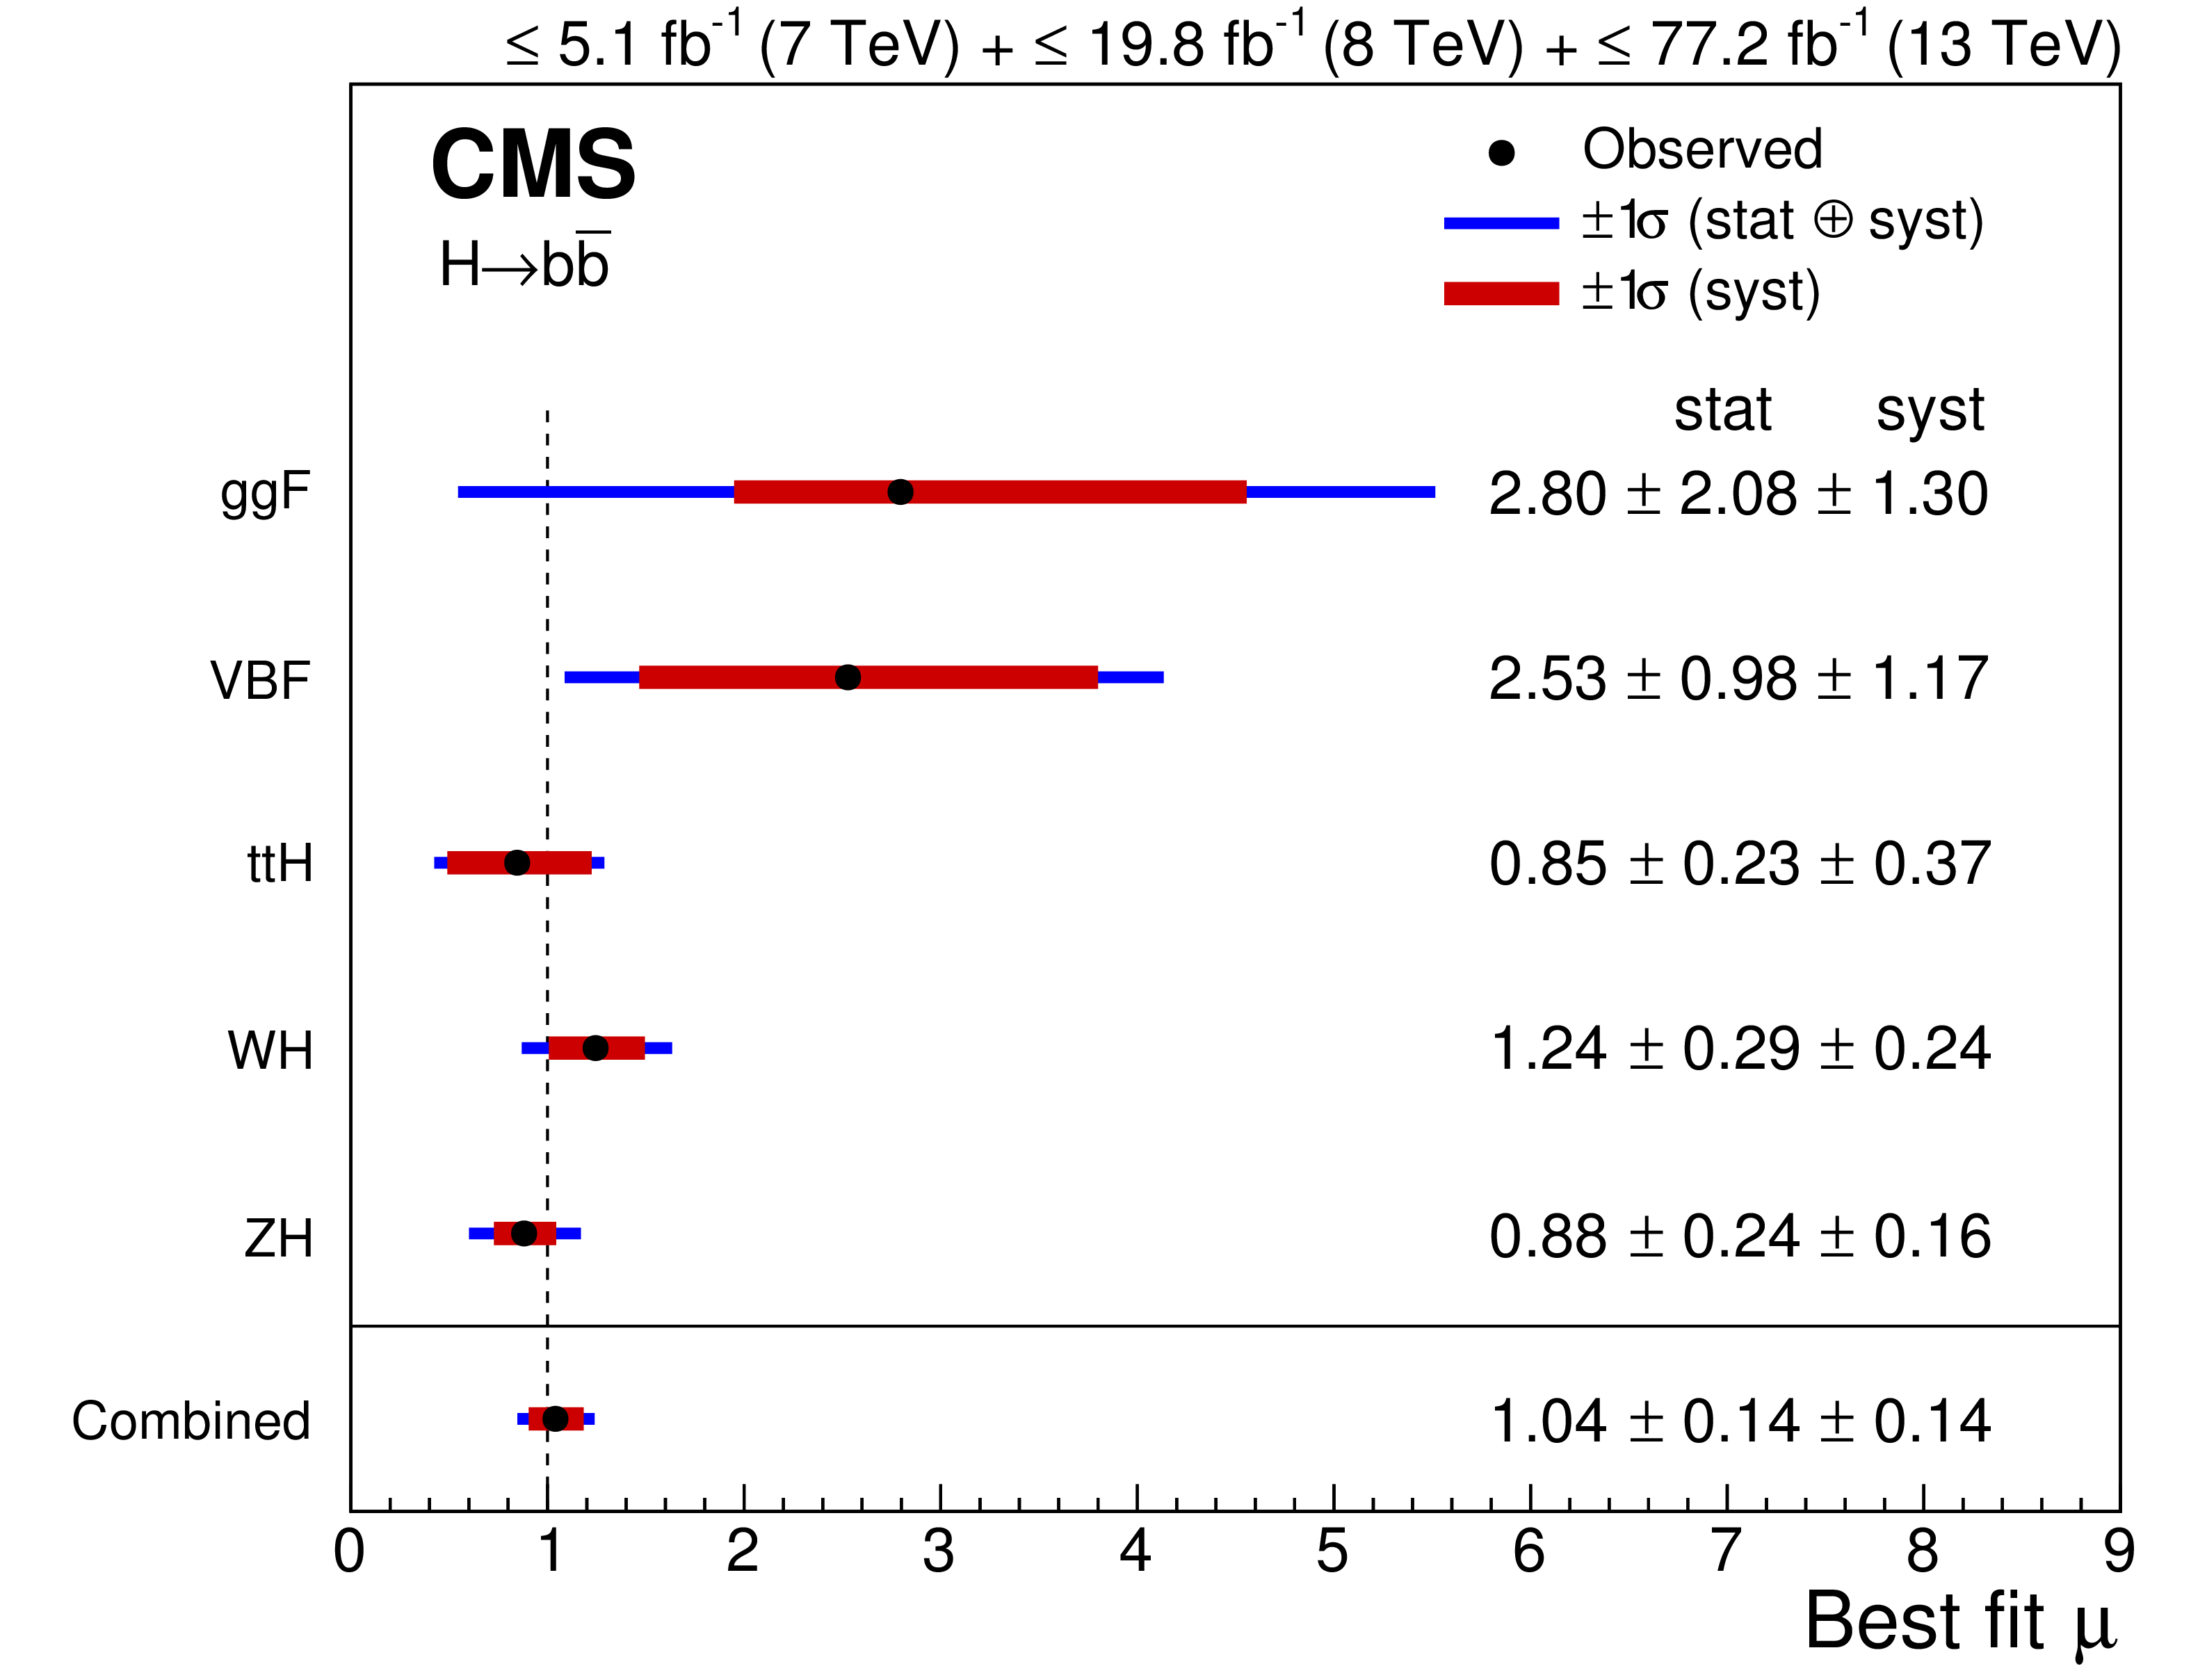
\includegraphics[width=3.5in]{images/CMS-HIG-18-016_Figure_003}
    \caption[\Hbb\ Combination Signal Strengths]{The best fit signal strengths and their uncertainties for each of the analyses of the different \Htobb\ production modes that participated in the grand combination.}
    \label{fig:MuHbb}
\end{figure}

